%%%%%%%%%%%%%%%%%%%%%%%%%%%%%%%%%%%%%%%%%%%%%%%%%%%%%%%
%%%%%%%%%%%%%%%%%%%%%%%%%%%%%%%%%%%%%%%%%%%%%%%%%%%%%%%

% The High-Granularity Calorimeter and HGCROC

% Description of the HL-LHC phase
% What are the main changes in the CMS detector that are expected for the HL-LHC?
% Description of the High-Granularity Calorimeter
% The read-out structure and HGCROC
% Description of HGCROC
% How can you characterize the chip?
% The irradiation test: TID and SEE
% Improvements in the chip design
% Conclusion

%%%%%%%%%%%%%%%%%%%%%%%%%%%%%%%%%%%%%%%%%%%%%%%%%%%%%%%
%%%%%%%%%%%%%%%%%%%%%%%%%%%%%%%%%%%%%%%%%%%%%%%%%%%%%%%

\chapter{The CMS Endcap Calorimeter Upgrade}
\label{chapter:The CMS Endcap Calorimeter Upgrade}

After nearly fifteen years of dedicated service, the LHC will undergo a major upgrade towards the High Luminosity LHC phase (HL-LHC), which is expecting to start its operations by the end of 2029.
The upgraded machine has been designed to operate at a  centre-of-mass energy of 14~TeV and to achieve a peak instantaneous luminosity of $L=5\cdot10^{34}\;cm^{-2}s^{-1}$: in these unprecedented running conditions, a remarkable integrated luminosity of 4000~$fb^{-1}$ is expected to be collected over the anticipated ten years of data-taking. 
With the HL-LHC upgrade, the amount of collected data will significantly increase, so as the potential for new discoveries at the LHC. The increased statistics will allow for more precise measurements of the SM properties but will also improve the potential for new discoveries, enhance the sensitivity to rare processes and possibly unveil the presence of previously unknown particles and BSM scenarios.

The higher luminosities of the HL-LHC will also result in exceedingly high pile-up rates, with $\mathcal{O}(200)$ events per bunch crossing and unprecedented radiation levels, with fluences of up to $3.5\times10^6\,\textrm{s}^{-1}\,\textrm{cm}^{-2}$ and a total absorbed dose of up to $\sim$$200\,\textrm{Mrad}$, thus posing several technical challenges for the operation of the detectors and the entire infrastructure.
In order to maintain its excellent physics performance in the high pile-up environment of the HL-LHC, the CMS Collaboration, as well as the other LHC experiments, is planning a series of major upgrades of the sub-detectors. The upgrade development and realization has already started during the Second Long Shutdown (LS2, 2018-2022) and will continue in the Third Long Shutdown (LS3, 2025-2029) when the installation and commissioning of the new detectors will be performed. 

\bigbreak

In this chapter, after a brief overview of the CMS upgrade plans in Sec.~\ref{sec:Upgrades of the CMS detector}, the focus will be directed towards the High Granularity Calorimeter (HGCAL), that will replace the current endcap calorimeters and completely renovate the CMS forward calorimetry strategy. The HGCAL detector, described in Sec.\ref{sec:The High-Granularity Calorimeter design} will provide the very first large-scale silicon-based imaging calorimeter employed in a high-energy physics experiment, with extremely fine transverse and longitudinal granularity, including a total of 6 million channels. Besides the unprecedented read-out segmentation, the performance requirements for the front-end electronics will be extremely stringent thus calling for ad-hoc electronics development. With an excellent technical effort to meet all these requirements, the HGCROC3 is the final version of the ASIC specifically designed to read-out the modules of the future HGCAL. 
The characteristics of the HGCROC will be described in Sec.~\ref{sec:The HGCAL Front-End Electronics}, while Sec.~\ref{FIXME} will present the irradiation campaigns performed on the chip to test its radiation hardness. 

\section{Upgrades of the CMS detector}
\label{sec:Upgrades of the CMS detector}

In the context of the future HL-LHC phase (Phase-2), the CMS detector upgrades programme has the main objective of maintaining the current physics performance under a new unprecedentedly complex environment. 
After years of operations, many current detector components have become inadequate to withstand high luminosity conditions and will either go through a complete replacement or a significant upgrade of already existing modules. There are three main points the CMS Collaboration has to consider to ensure that the detector's capabilities align with the ambitious research goals of the HL-LHC era:
\begin{itemize}
    \item [-] The unprecedented radiation doses will necessitate a complete replacement of the tracker and endcap calorimeter systems, the adoption of new technologies for the electromagnetic barrel (EB), and substantial enhancements to the electronics systems in the barrel calorimeters and muon detectors.
    \item [-] The increase in the pile-up rate will require highly granular read-outs wherever possible, the implementation of precision timing detectors, and innovative approaches to pile-up mitigation.
    \item [-] The high luminosity will result in an increased data stream, highlighting the crucial need for substantial improvements to the L1 Trigger primitives and the overall Trigger and Data Acquisition System (TriDAS).
\end{itemize}

To enhance the detector's granularity and reconstruction performance while minimizing the material budget, the tracking system will be entirely replaced. This involves employing smaller pixel detectors for the inner tracking system and incorporating strips and macro pixel sensors for the outer tracking stations, extending coverage up to $|\eta|=3.8$. These changes are expected to improve longitudinal and transverse resolutions, as well as reduce fake rates, enabling the reconstruction of L1 trigger tracks up to $|\eta|=2.4$.

The endcap calorimeters will be replaced with the HGCAL, a high-granularity sampling calorimeter designed to enhance shower separation, particle identification, and provide precise timing information.

Additionally, to increase granularity and provide supplementary timing measurements, upgrades to the ECAL and HCAL barrel electronic read-out systems are planned. 

The redundancy of the current muon detection system, comprising DTs, RPCs, and CSCs, will be augmented by the installation of Gas Electron Multiplier chambers and a new generation of RPCs. These enhancements will extend coverage up to $|\eta|=2.8$ and $|\eta|=2.4$, respectively.

Furthermore, multiple MIP timing detectors (MTD) will be positioned in front of the barrel and endcap calorimeters. This additional layer will improve the timing information on charged candidates, which is crucial for disentangling the approximately 200~PU interactions foreseen per bunch crossing.

Finally, the trigger and data acquisition systems will be completely replaced, redesigning the Level-1 hardware trigger to include tracking and high-granularity calorimeter information exploited via the extensive use of state-of-the-art FPGAs and ML techniques.

\bigbreak

Figure~\ref{fig:CMSUpgrade} illustrates a cross-section of the CMS detector, outlining the planned upgrades for the HL-LHC. For each subdetector, the the main modified features are described: the Tracker, TriDAS system and the forward calorimeters will undergo complete replacement, while the MIP timing detector, the barrel calorimeters and the muon system will constitute new parts or modules that are not part of the current CMS design.
% https://cds.cern.ch/record/2628519

\begin{figure}
    \centering
    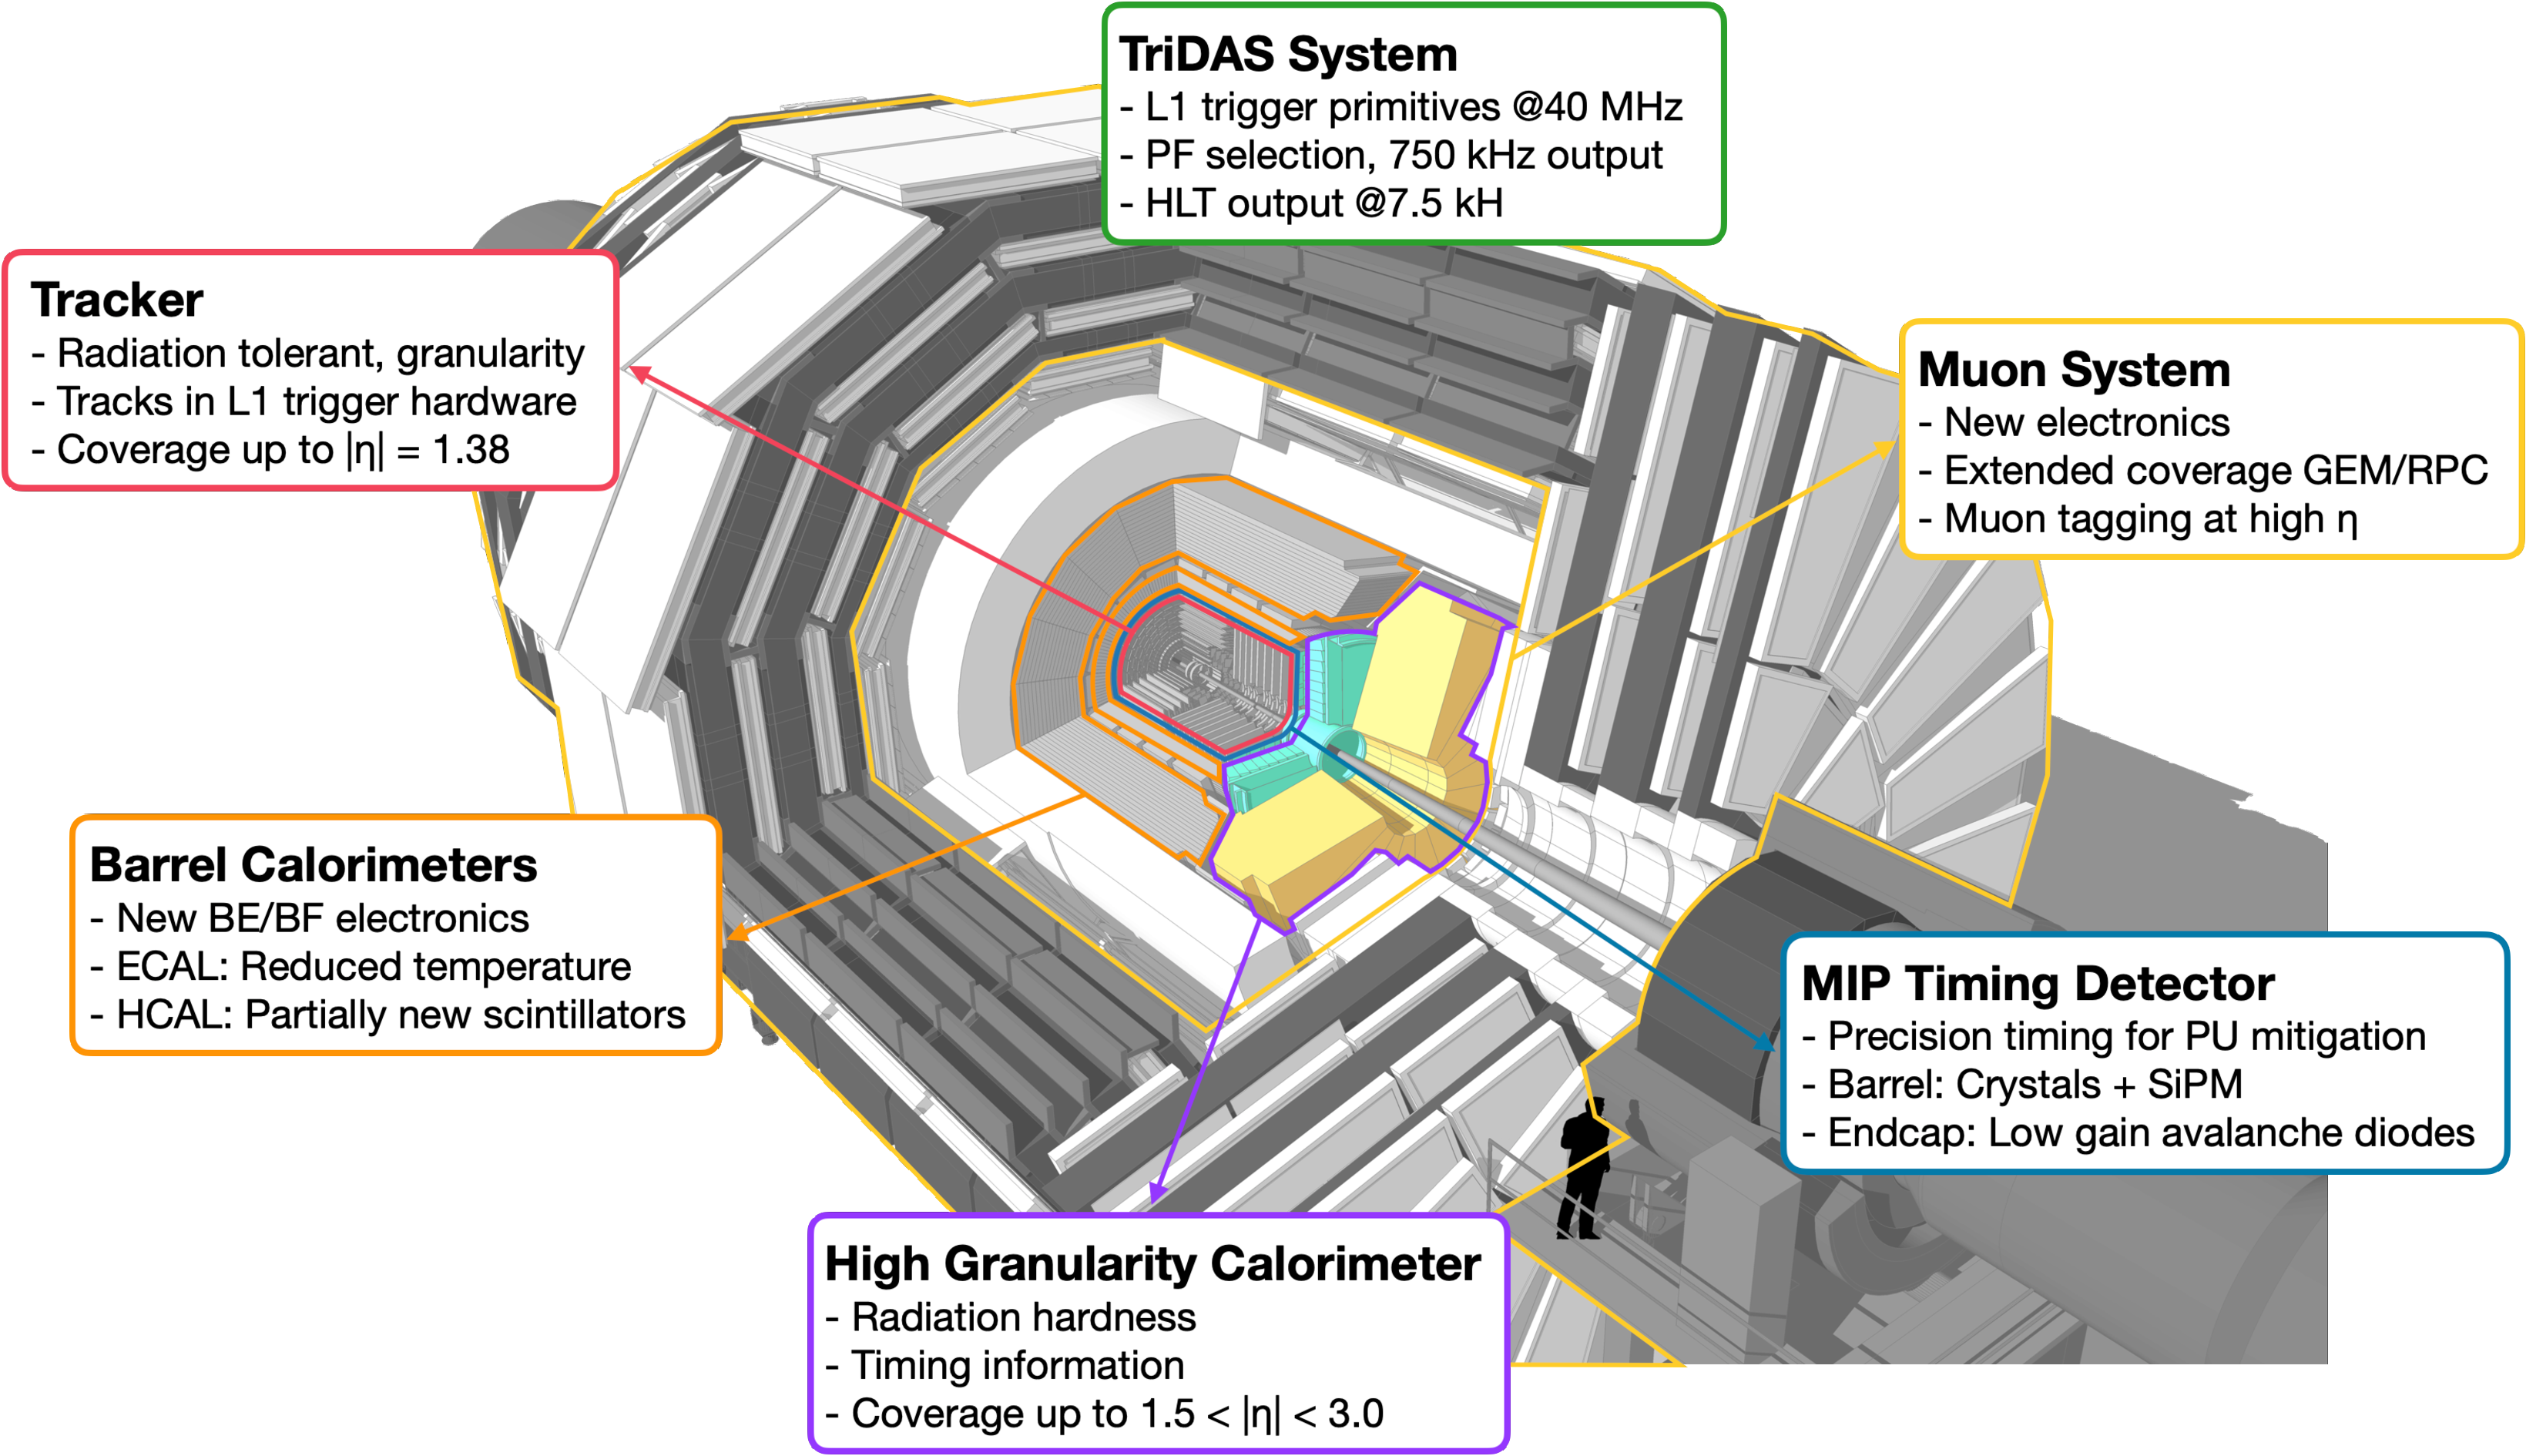
\includegraphics[width=0.95\linewidth]{Figures/HGCAL/CMSUpgrades.pdf}
    \caption{Cross section of the CMS detector with the indication of the upgrades foreseen for the HL-LHC.}
    \label{fig:CMSUpgrade}
\end{figure}

\section{The High-Granularity Calorimeter design}
\label{sec:The High-Granularity Calorimeter design}

Among the CMS detector updates, one of the most ambitious projects is the High Granularity Calorimeter (HGCAL), a high-granularity sampling calorimeter designed to replace the existing CMS endcap calorimeter in order to to maintain a excellent physics performance under the high pile-up and harsh radiation environment of the HL-LHC.

The existing $\textnormal{PbWO}_4$-based Endcap Calorimeters (CE) of the CMS detector were designed to sustain a total integrated luminosity of 500 $\textnormal{fb}^{-1}$. 
The transparency of the lead-tungstate crystals, already degraded during Run-II operations, would not survive the unprecedented radiation flux typical for the HL-LHC environment in this detector region.
It is therefore necessary to replace the current calorimeter endcaps with a new detector with high radiation tolerance, highly granular energy deposit and good time resolution to adequately treat pile-up in the offline event reconstruction. \newline

The HGCAL will consist of 47 layers divided into two compartments:
\begin{itemize}
    \item [-] the Electromagnetic Compartment (CE-E), featuring 26 active layers, interspersed with CuW, Cu, and Pb absorbers,
    \item [-] the Hadronic Compartment (CE-H), composed of 21 layers exploiting stainless steel as passive material.
\end{itemize}

The number of longitudinal samplings has been designed as a trade-off between the best shower reconstruction and the engineering requirements of the mechanical structure. 

To meet the radiation hardness requirements, the CE-E and the front part of the CE-H will employ silicon as active material, for a total area of about 600~$\textnormal{m}^2$ to be covered. In the remaining lower radiation regions of CE-H, at about 4~m from the interaction point, segmented plastic scintillators with silicon photomultipliers (SiPM) for the read-out will be used as the active material. Squared scintillator tiles with sizes ranging from 4~$\textnormal{cm}^2$ up to 30~$\textnormal{cm}^2$ will be installed, for a total of about 400~$\textnormal{m}^2$ of active area covered in scintillators.

This configuration amounts to a total of 10 nuclear radiation lengths ($\lambda_n$), divided into 1.3~$\lambda_n$ for the CE-E and 8.5~$\lambda_n$ for the CE-H. The CE-E alone will extend for a total of 27.7 radiation-lengths ($X_0$).
To further improve radiation resistance, the full system is cooled down to 240~K ($-30^{\circ}$C) with liquid $\textnormal{CO}_2$.

\begin{figure}
    \centering
    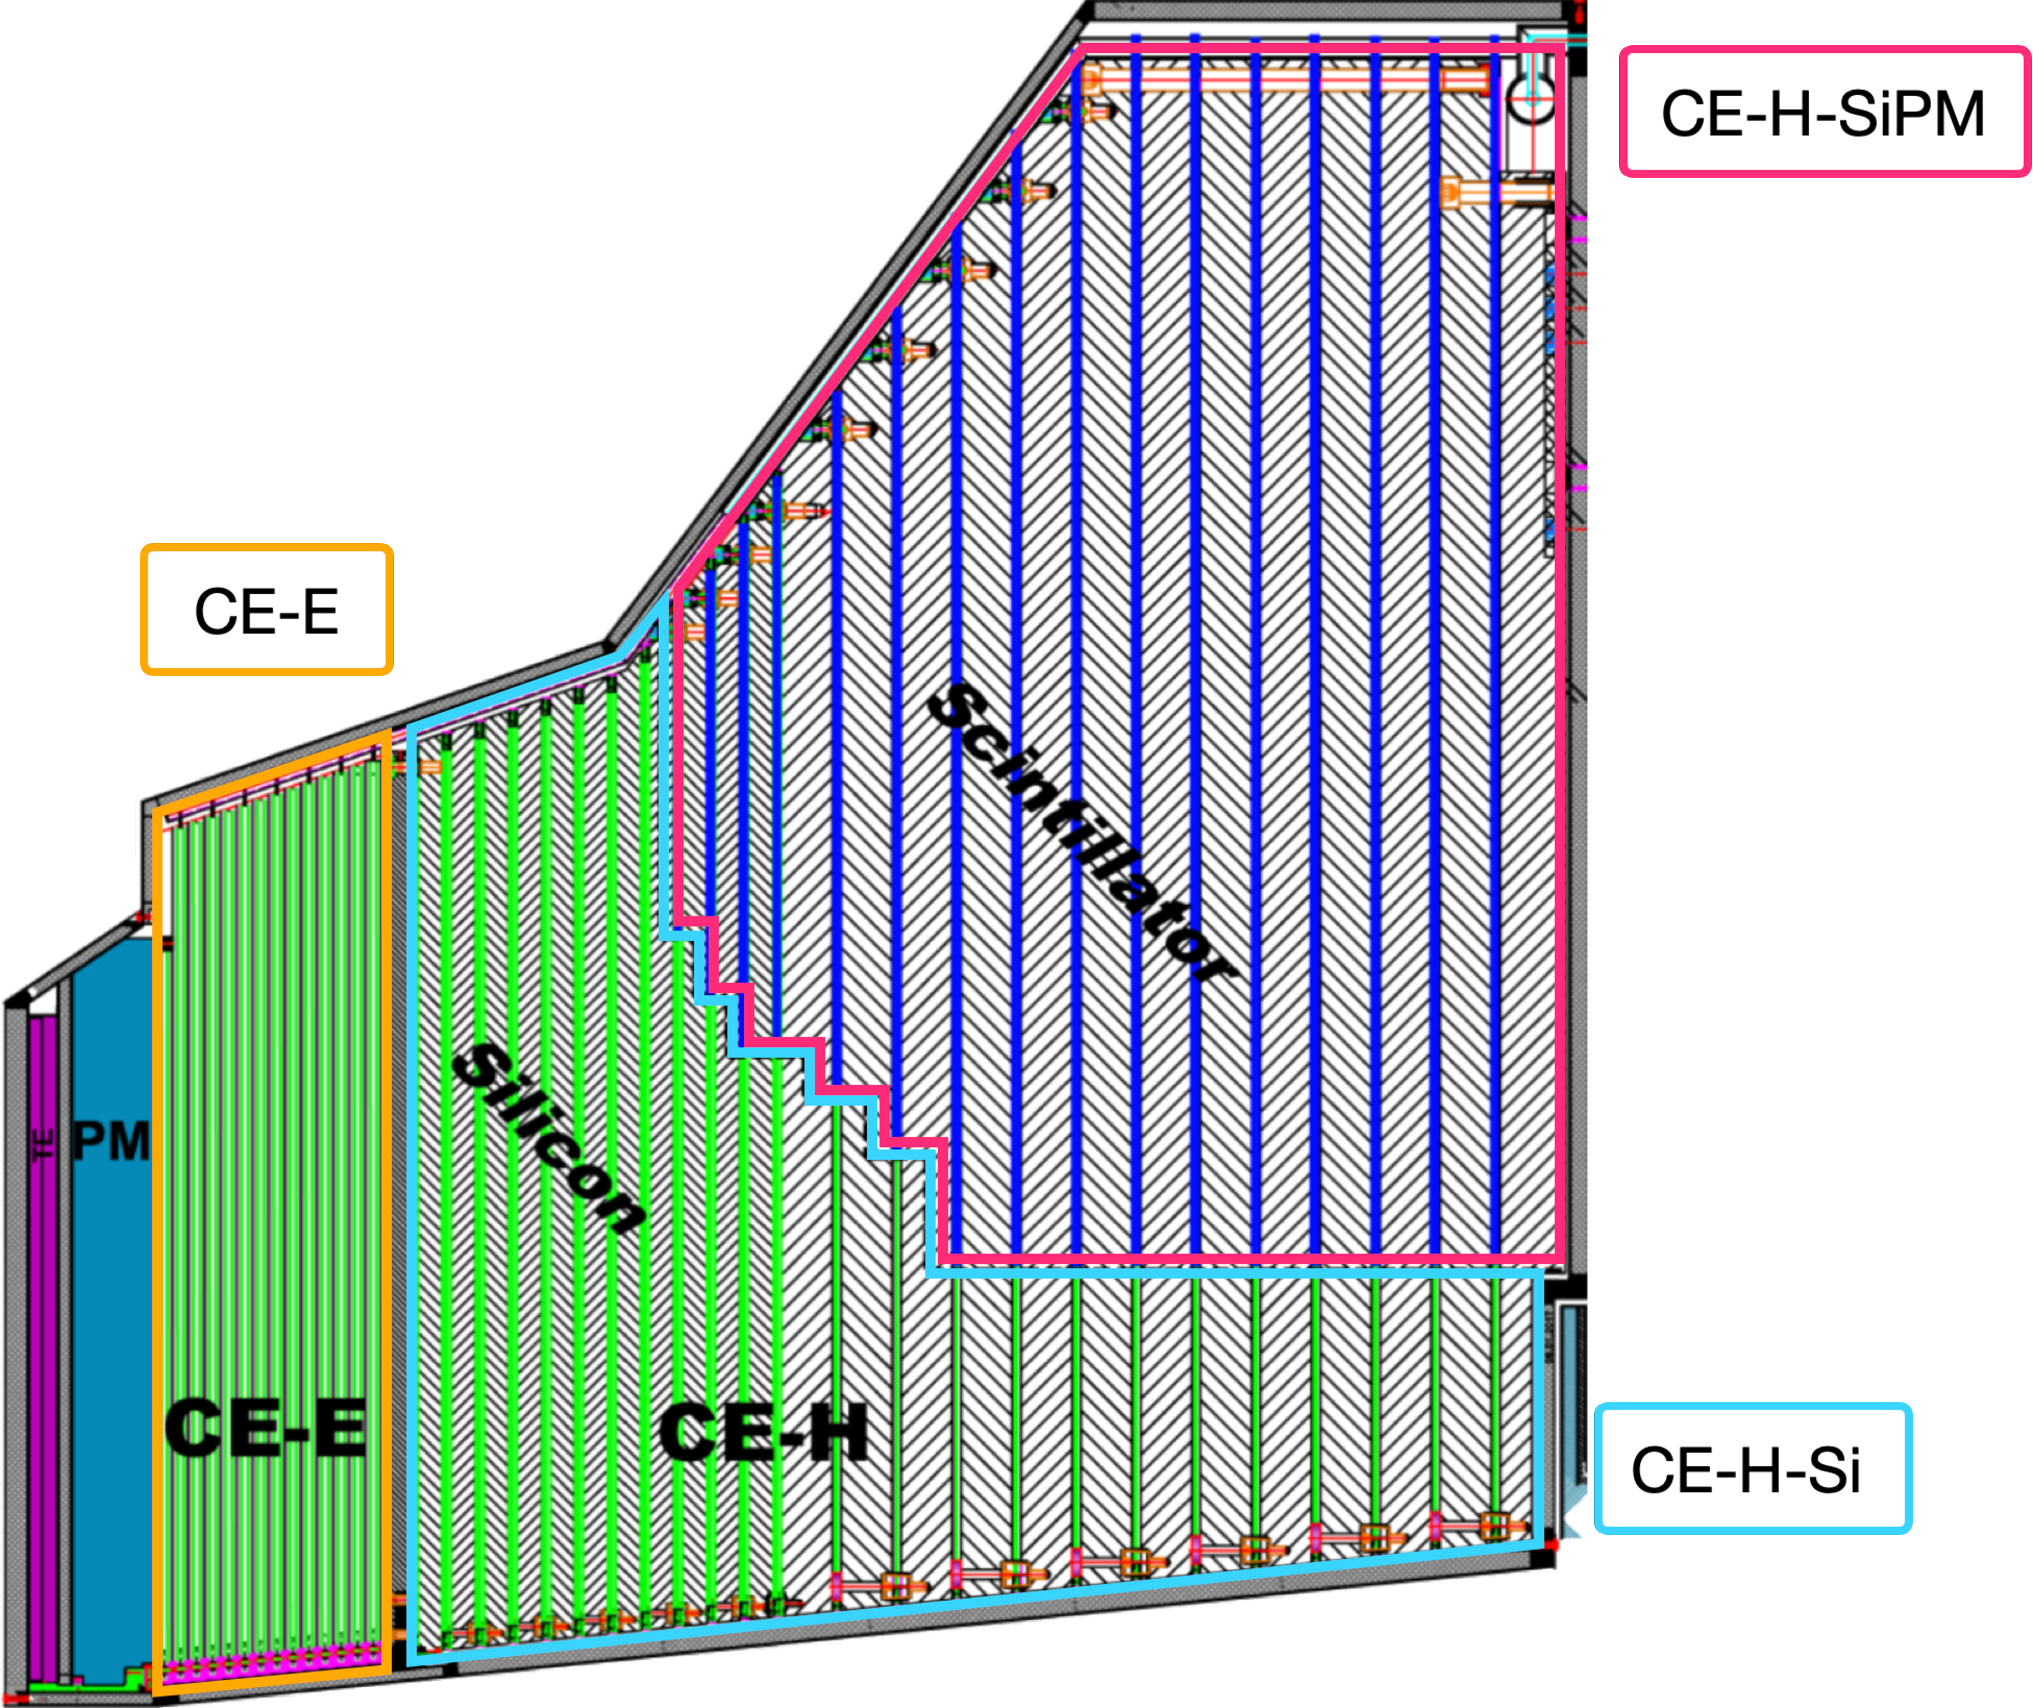
\includegraphics[width=0.6\linewidth]{Figures/HGCAL/HGCALLayers.pdf}
    \caption{Cross section view of the HGCAL. The CE-E and front CE-E compartments comprise silicon-based components. In its latest design, it features 47 layers divided into two regions: 26 silicon-based layers for the Electromagnetic Compartment (CE-E), 21 layers for the Hadronic Compartment (CE-H) using silicon (CE-H-Si) and scintillator-based (CE-H-SiPM) active material. The expected coverage of the HGCAL will range from $|\eta|=1.5$ up to $|\eta|=3.0$.}
    \label{fig:HGCALLayers}
\end{figure}

A longitudinal cross section of the HGCAL is shown in Fig.\ref{fig:HGCALLayers}, where the multiple layers if the Electromagnetic and Hadronic Compartments are visible, along with the different active material used in the two regions.

\bigbreak

In order to cover the area in the most cost-effective manner, the hexagonal geometry for the silicon sensors will be exploited. To reduce the number of modules, the baseline of the sensor size has been adjusted from the initially foreseen 6\mbox{''} design to 8\mbox{''}. An active thickness of 120, 200, or 300 $\mu$m is expected, depending on the detector region.
Each module will comprise several single read-out diodes, hereafter referred to as \textit{cells}, with a 0.5 or 1.0~$\textnormal{cm}^2$ active area, for a total of about six million cells to read out individually in the ultimate detector operation. 
The design, production, and validation of these hexagonal sensors, hereafter referred to as \textit{modules}, is one of the most challenging aspects of the HGCAL project. A more detailed discussion about silicon as active material and the structure of the HGCAL modules is given in Sec.~\ref{sec:Silicon Modules}. 

In the CE-E, the silicon modules will be used to create self-supporting sandwich structures which are commonly referred to as \textit{cassettes}. For this, the modules will be installed on both sides of a copper cooling plate and will be closed with lead plates.

In the low radiation CE-H-SiPM compartment, the scintillating material coupled to SiPMs read-out will be transversely segmented in square shapes with the size of 4 to 30~$\textnormal{cm}^2$, depending on the pseudorapidity position. 
The scintillator modules will be composed of tileboard printed circuit boards (PCBs) with different sizes and shapes. Each tileboard will host from 48 to 96 scintillator tiles individually wrapped into a reflecting layer and characterised by a cavity to contain the SiPM. Each detector on the board will be equipped with an ultraviolet LED next for the calibration and monitoring of the SiPM gain. 

This geometrical configuration amounts to a total active area of 620~$\textnormal{m}^2$ and 370~$\textnormal{m}^2$ for the CE-E and CE-H compartments respectively and provides a compact and cost-effective way to build the entire calorimeter at a reasonable cost while meeting the strict radiation requirements in the high pseudorapidity region.

\begin{figure}
    \centering
    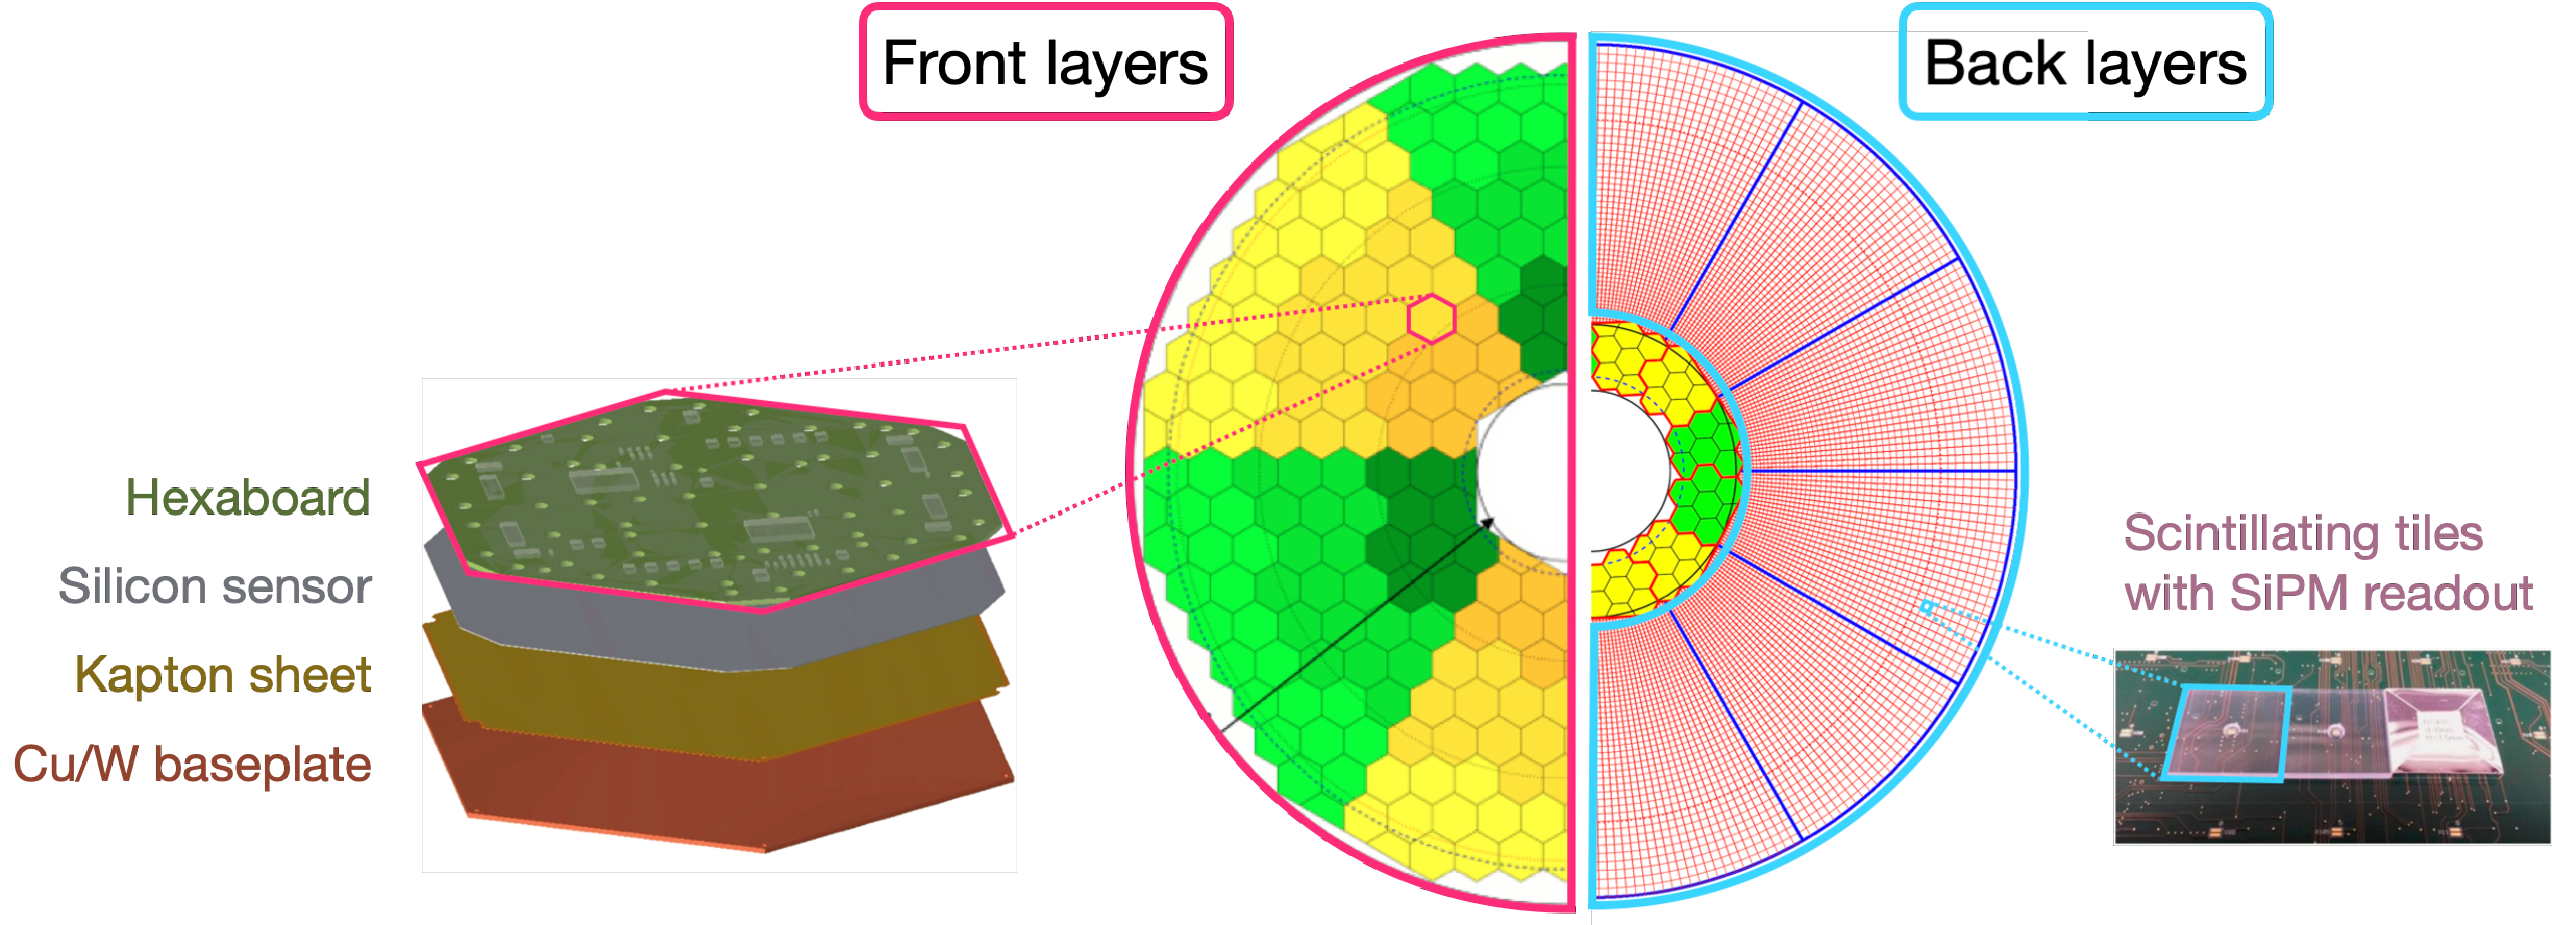
\includegraphics[width=0.9\linewidth]{Figures/HGCAL/FrontBackLayers.pdf}
    \caption{Schematic view of the arrangement of the hexagonal silicon modules in the front layers composing the CE-E and CE-H-Si (left) and of the scintillator tiles employed in the low radiation back layers of the CE-H-SiPM (right).}
    \label{fig:FrontBackLayers}
\end{figure}

The arrangement of the silicon modules in the CE-E and CE-H-Si (front layers) is represented in the left part of Fig.~\ref{fig:FrontBackLayers}, while the right part shows the scintillator tiles employed in the CE-H-SiPM region (back layers).

\bigbreak

The HGCAL design guarantees coverage in the pseudorapidity range $1.5 < |\eta| < 3.0$, featuring both highly granular lateral and longitudinal segmentation. 
The enhanced lateral granularity, combined with the dense absorbers, yields effective individual shower discrimination within the detector. Moreover, the finely segmented longitudinal structure enhances PU rejection, particle identification, and energy resolution. Because of these features, the HGCAL is often referred to as an \textit{imaging}, or 5D, calorimeter, the five dimensions corresponding to the three-dimensional spatial information provided by the fine voxels, the energy deposit in each active material segments, and the timing information with an expected resolution of $\mathcal{O}$(10 ps).

The calibration of the detector will be performed with minimum ionizing particles (MIP). To maintain a reasonable detection of MIPs over the detector's lifetime and ensure a signal-to-noise ratio above one, the effects of radiation damage must be minimized. To achieve this, the HGCAL will have to be operated at a constant temperature of -30~$^{\circ}$C or lower, obtained through a dedicated $\textnormal{CO}_2$ cooling system directly implemented in the copper base plate. 

\subsection{Silicon Modules}
\label{sec:Silicon Modules}

The choice of silicon as the active material in the HGCAL modules is driven by the stringent constraints imposed by the expected physics performance and operating conditions of the detector. 
Silicon sensors ensure the detection of minimum ionizing particles (MIPs) and facilitate precise measurement of high-energey showers, both crucial for the HGCAL's operation efficiency. The former is essential for \textit{in situ} calibrations of the detector, while the latter can be ensured only with a full containment of the showers, which relies on the detector compactness achieved through thin silicon modules and a proper mixture of absorbers.

These requirements are met by silicon sensors, which offer rapid signal response $\mathcal{O}$(10 ns) necessary to keep up with the expected 40 MHz rates at the HL-LHC. Additionally, silicon module production benefits from established large-scaled industrial capabilities, allowing for relatively short lead times.

The validation of the silicon modules structure has been cornerstone of the project since the approval of the HGCAL Technical Proposal (TP) in 2015. Several proof-of-concept modules, produced by Hamamatsu Photonics K.K. (HPK), have undergone extensive testing in beam experiments between 2016 and 2017. Insights from these tests, incorporated into the 2018 HGCAL Technical Design Report (TDR), form the foundation for understanding the properties of silicon modules crucial for such a complex detector.

\bigbreak

The HGCAL will require approximately $27\,000$ silicon detector modules to be assembled and installed in its electromagnetic (CE-E) section and part of the hadronic (CE-H) section.

Each module consists of stacked layers comprising the printed circuit board (PCB), labeled \textit{hexaboard}, where the front-end electronics are installed, a silicon sensor, and a gold-plated Kapton sheet providing HV connection to the sensor back-plane and electrical insulation. The baseplate, made of materials such as CuW or Cu, provides enough rigidity to support the module whilst minimizing the total radiation length and dissipating the heat through a dedicated cooling system.

The silicon modules will be further segmented into either 192, for low-density (LD), or 432 individual diodes, for high-density (HD) modules. The diodes will act as sensor cells and have a separate read-out channel.

\begin{figure}
    \centering
    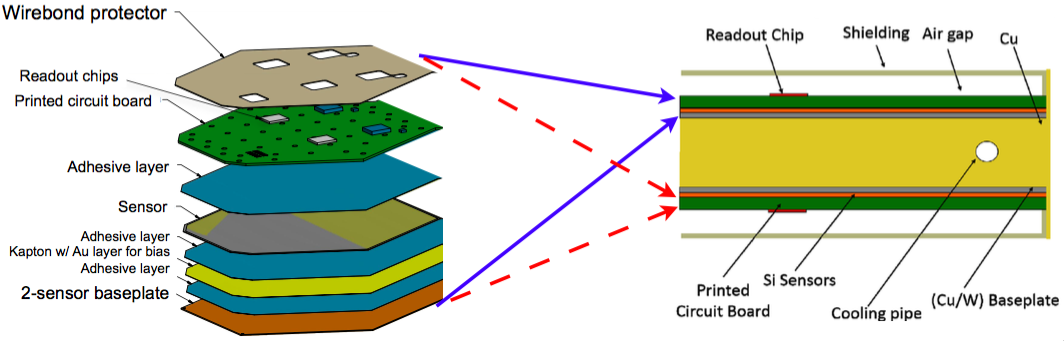
\includegraphics[width=0.9\linewidth]{Figures/HGCAL/ModuleDesign.png}
    \caption{Composition of a silicon module and placement in the copper plate. Each module is a stack of different layers, starting with a baseplate at the bottom, covered with a gold plated Kapton foil on which stands the silicon sensor. A protected PCB with read-out chip is placed on top.}
    \label{fig:ModuleDesign}
\end{figure}

A schematic view of the structure of a typical HGCAL module is given in Fig.~\ref{fig:ModuleDesign}.

\subsection{Plastic Scintillation Tiles}
\label{sec:Plastic Scintillation Tiles}

The remaining portion of the CE-H compartment will incorporate scintillator as the active material in regions where the integrated dose remains low-enough ($<3$~kGy) to maintain optimal performance throughout the entire lifespan of the HL-LHC. 
This approach will also ensure effective muon identification in the $\eta>2.4$ region, where muon chambers are not available.

The scintillator will be crafted into small squared tiles, with the scintillation light reflected by a wrapping foil and directly read-out by a SiPM optically coupled through a small \textit{dimple} in the centre of one face of each tile. The SiPMs will be mounted on printed circuit boards, matched to the appropriate tiles. 
The system is illustrated in Fig.\ref{fig:ScintillatorTiles}.

In conformity with the CMS endcap's geometry, the scintillator cells will be arranged in an $r,\phi$ grid. As a result, cells closer to the beam line will be significantly smaller (4~$\textnormal{cm}^2$) than those at the outer edge (32~$\textnormal{cm}^2$). 

The area instrumented with scintillator will be subdivided into tile-modules consisting of a tileboard and the scintillator tiles. These tile-modules will then be connected together to form a 10~$^{\circ}$ detector unit. Six such units will be placed next to each other and combined with silicon modules into cassettes, covering 60~$^{\circ}$ each. Finally, six cassettes will collectively complete the calorimeter layer around the beam pipe.

\begin{figure}
    \centering
    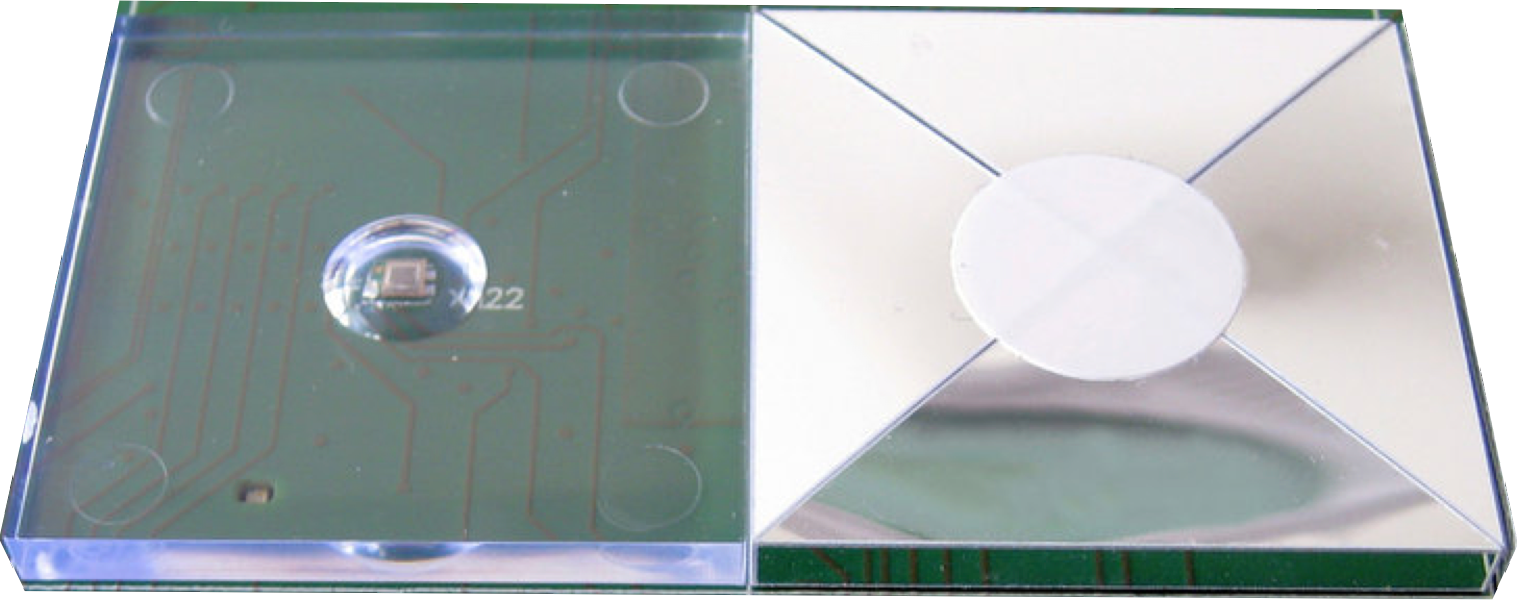
\includegraphics[width=0.5\linewidth]{Figures/HGCAL/ScintillatorTiles.pdf}
    \caption{Example of two $3\times3\textnormal{cm}^2$ scintillator tiles with a central dimple, unwrapped (left) and wrapped (right), mounted on a PCB housing one SiPM per tile, used as a prototype for the HGCAL project.}
    \label{fig:ScintillatorTiles}
\end{figure}

\section{The HGCAL Front-End Electronics}
\label{sec:The HGCAL Front-End Electronics}

One of the most challenging aspects in the design of the HGCAL silicon and scintillator modules is the front-end (FE) electronics. 

The FE electronics is responsible for several critical functions within the HGCAL system. It measures and digitizes the charge deposited in the silicon sensor pads or generated in the SiPMs, providing precise time measurements for the pulses. It transmits the digitized data to the back-end (BE) electronics located in the service cavern. It also computes, at each bunch crossing, the digital sums of neighboring cells, tailored to the specific cell sizes ($2\times2$ cells for 1~$\textnormal{cm}^2$ pads silicon sensors, 3 cells for 0.5~$\textnormal{cm}^2$ sensors, and 2 cells for scintillator tiles) to be transmitted to the trigger BE electronics to build trigger primitives.

Besides the unprecedented readout segmentation, the performance requirements for the FE electronics are extremely stringent, particularly for the silicon part of the detector:
\begin{itemize}
    \item [-] Low noise and large dynamic range, spanning from approximately 0.2~fC to 10~pC, equivalent to 16 bits. This range enables the detection of MIPs in the silicon sensors and recording of high-energy deposits from electromagnetic showers. 
    The electronics noise must be below 2000 electrons for a 65~pF capacitance pad to allow MIP visibility during the whole operation.
    \item [-] Integral linearity must exceed 1$\%$ across the entire dynamic range.
    \item [-] Timing information with a precision better than 100~ps for pulses above 12~fC, corresponding to about 3~MIPs in the 300~$\mu$m silicon sensors.
    \item [-] Fast shaping time (peaking-time $<20$~ns) to minimize the out-of-time pileup: the pulse should be dropped to less than 20$\%$ by the next bunch crossing.
    \item [-] On-detector digitization and data processing for zero suppression, linearization and summing of the trigger data.
    \item [-] Maximum latency of 36~bunch crossings for the trigger primitives at the output of the detector.
    \item [-] Buffering of the data to accommodate the 12.5~$\mu$ms latency of the L1 trigger.
    \item [-] High-speed read-out links to interface with the 10~Gb/s low-power GBT (LpGBT) serializer.
    \item [-] Low power budget ($<20$~mW per channel), typically limited by cooling power.
\end{itemize}

Following the LHC data-taking conditions, the acquisition chain must handle consecutive event arrivals at 40~MHz without data erasure.
Moreover, the FE electronics will face a harsh radiation environment which will reach 200~Mrad at the end of life and requires good radiation tolerance.

\begin{figure}
    \centering
    \includegraphics[width=0.95\linewidth]{Figures/HGCAL/Hexaboards.pdf}
    \caption{Plan view of two hexaboards housing 6 High Density (HD) HGCROC read-out chips: each chip is connected to 72 hexagonal cells. The connector will be used for the assemply of the motherboard, containing the ECON-D and ECON-T concentrator chips.}
    \label{fig:Hexaboards}
\end{figure}

\bigbreak

The very first step of the FE electronics read-out chain is the HGCal Read-Out Chip (HGCROC), which measures the charge and the time of arrival at 40~MHz frequency. The HGCROC is directly bonded through a ball-grid array to the hexaboard and has multiple channels connected to individual cells. 
The read-out chips, the linear voltage regulators (LVR), and any other passive and service components are mounted on a hexagonal module PCB, called \textit{hexaboard}, which is glued onto the silicon sensor. Imprinted on the hexaboard are also the pads for connections to the next board in the chain, labeled \textit{motherboard}. Through these connections also supply the LV, and the received and transmitted signals and data. 

\bigbreak

The next level of the FE electronics includes the concentrators, located on motherboards sitting 1.6~mm above the hexaboards. A motherboard serves from one to six modules, depending on the occupancy of the sensors. The surfaces which include the components of the hexaboard and of the motherboard face each other in order to reduce the overall thickness. 

The architecture of the very FE electronics chain on the hexaboards is summarised in Figure~\ref{fig:Hexaboards}. 

\section{The HGCROC3 architecture}
\label{sec:The HGCROC3 architecture}

With an extraordinary technical effort to meet all these requirements, the HGCROC3 is the final version of the ASIC specifically designed by the CMS Collaboration, in collaboration with the Omega Microelectronics Center at École Polytechnique, to read-out the modules of the future HGCAL. 
Two versions of the same readout architecture have been developed, for the silicon (Si) and the scintillator tiles (SiPM) sections, where the latter is obtained by only adding a current conveyor and adapting the preamplifier of the silicon variant.

\bigbreak

The main function of the HGCROC3 is to measure and digitize the charge deposit and provide high precision time information of the particles crossing the detector layers. It is also able to compute the energy sum of neighbouring cells in order to contribute to the Level-1 (L1) trigger decision. 
The chip features 78 channels, each consuming less than 15 mW power, and is designed in a radiation-hardened 130~nm CMOS technology. Among the channels, 72 serve as standard cell read-outs, 2 function as calibration cells read-out, and the remaining 4 channels are not connected to any sensor cells, serving for common-mode noise estimation. 

The layout is symmetrically divided into two parts, of \textit{halves}, as shown in Fig.~\ref{fig:TowHalves}.
In Fig.~\ref{fig:Architecture} a schematics of the inner architecture of the ASIC is presented: the structure and characteristics of each component are described in the following paragraphs.

\begin{figure}
    \centering
    \includegraphics[width=0.75\linewidth]{Figures/HGCAL/TwoHalves.pdf}
    \caption{Layout of the HGCROC3 ASIC: the chip is divided into two symmetrical parts. The voltage reference is positioned near the chip's edge, the ADC reference and TDC controls are located in the central region.}
    \label{fig:TowHalves}
\end{figure}

\paragraph{Data path}
The data path is the core of the chip, replicated for 72 channels of the full analog chain, 4 common mode channels for the coherent noise subtraction, and 2 calibration channels for the MIP calibration. This component extracts from the signal input charge three digitised quantities to be sent to the back-end electronics: the ADC for the charge measurement, the ToA (Time-of-Arrival) for the time measurement, and the ToT (Time-over-Threshold) for the charge measurement of saturated signals. 

The charge digitization is achieved by a 10-bit~ADC in the linear range of the preamplifier; when it saturates, a 12-bit Time-to-Digital Converter (TDC) with 50~ps binning over 200~ns range provides the charge information by measuring the ToT. The ToA digitization is carried out by a similar dedicated 10-bit TDC with 25~ps binning over 25~ns range.
The low-noise preamplifier gain can be adapted to different detector regions, where the MIP energy deposit can vary depending on the sensor thickness and irradiation condition.
Under HL-LHC conditions, certain regions of the detector may exhibit notably high occupancy rates, reaching up to 50$\%$ of fired cells per bunch crossing: it is thus important that the analog shaper drops the signal sample to less than 20$\%$ by the next bunch crossing to mitigate the out-of-time pile-up.

Beyond the analog performance, the chip embeds a large part of digital processing to manage the Data and the Trigger paths. A 512-depth DRAM (RAM1) is used as a circular memory to buffer the data to accommodate the 12.5~$\mu$s latency of the L1 trigger, and a 32-depth DRAM (RAM2) is used as a FIFO after the L1 selection.
Two 1.28~Gbps links are dedicated to send out the full event information of the selected bunch crossings after a L1 request.

\begin{figure}
    \centering
    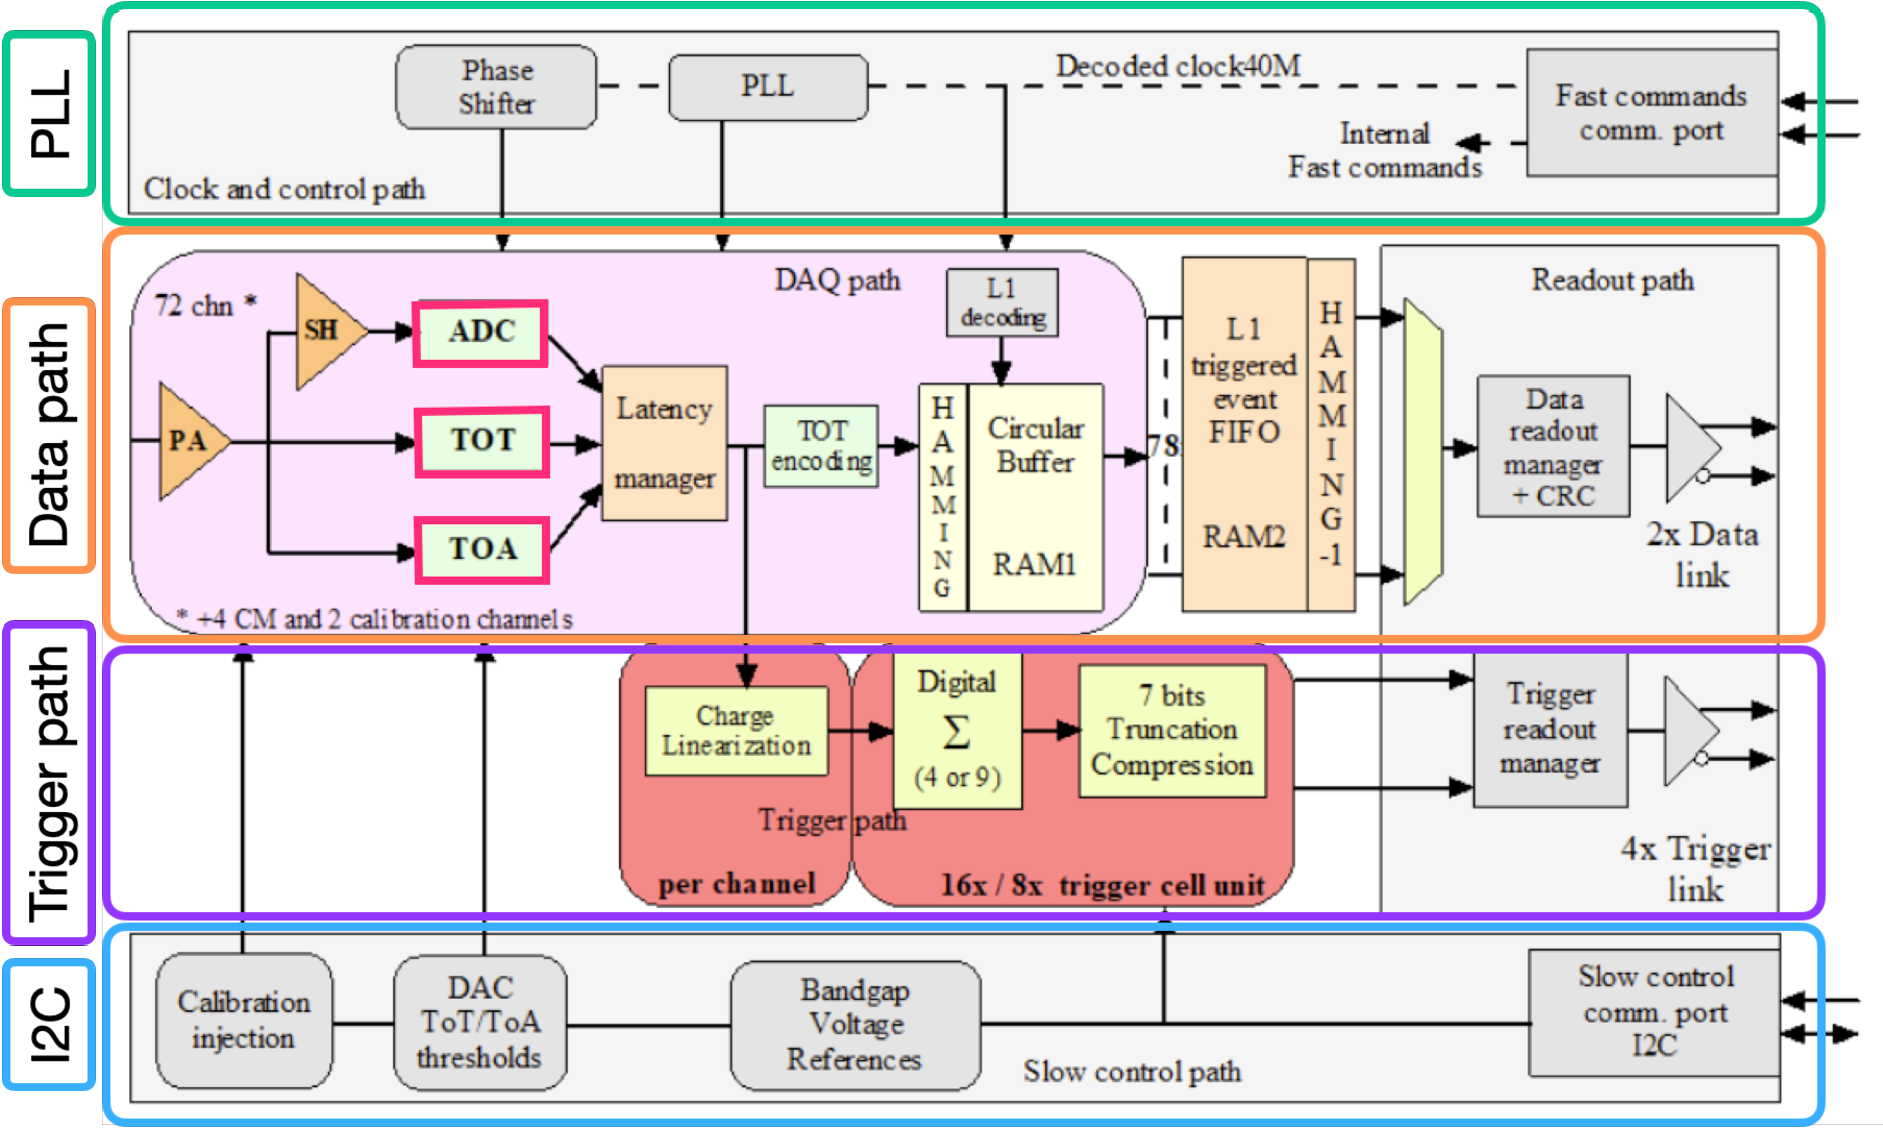
\includegraphics[width=0.75\linewidth]{Figures/HGCAL/Architecture.pdf}
    \caption{Architectural overview of the HGCROC3 read-out ASIC. The main parts composing the Data path, Trigger path, PLL and I2C have been highlighted.}
    \label{fig:Architecture}
\end{figure}

\paragraph{Trigger path}
The trigger path computes an image of the deposited charge at each bunch crossing, by summing and compressing data over neighbouring channels. The two charge-related quantities from the channel information (ADC and ToT) are fed into the trigger path. The chip performs the data processing with a charge linearisation over the ADC and ToT range and computes the energy sums over 4 (9) adjacent channels for the LD (HD) modules. After compressing the information to 7 bits, it sends the trigger data to the ECON-T concentrator chip.
Four $1.28\,\textrm{Gbps}$ differential links are devoted to send the energy sums for the L1 trigger decision. The data are sent to the ECON-T concentrator chip.

\paragraph{PLL}
The Phase-Locked Loop (PLL) is an analog clock synthesizer receiving the 40~MHz LHC clock and providing all the other clock frequencies - from 160~MHz to 1.28~GHz - used by the circuit.
The main challenge for the PLL circuit is to ensure that all the clocks' phases are aligned to the LHC 40~MHz input clock: a low noise digital Phase Frequency Detector (PFD) continuously checks for possible phase misalignments and, in case one is found, the chip adjusts the voltage-controlled oscillator (VCO) in order to temporarily increase or decrease the frequency and realign the phase. The PLL is an essential component for the HGCROC3 functioning and has been intensivley tested during the irradiation campaigns, as described in Sec.\ref{FIXME}.

\paragraph{I2C}
The Inter-Integrated Circuit (I2C) is an internal static memory register storing the chip's configuration parameters.
The I2C protocol is used to set or read the more than 7900 parameters, distributed into 8 internal registers.
A Fast Command block is used to read and write the configuration parameters, to configure the operating mode of the system (link synchronisation, reset, calibration, L1 request, etc.), and to communicate with the device.

\section{Characterisation and testing of the HGCROC3}
\label{sec:Characterisation and testing of the HGCROC3}

% When I arrived the new  HGCROC3 had just arrived and we had to test their performance in order to check whether the met the requirements
% What are the differences between HGCROC2 and 3?

The characterisation of the HGCROC3 is a crucial step towards validating the chip's design, ensuring expected performance within the acceptable limits and reliability in the operations.
This section outlines the main procedures for calibrating and testing the HGCROC3, which will be essential to comprehend its performance in preparation for the irradiation testing.

% \bigbreak

% There are different set-ups:
% - HGCROC3 on the mezzanine board, on which all the power supplies remain separated and it is possible to check the performance of the circuit in an optimistic framework (possible couplings via power supplies are reduced).
% - HGCROC3 in a mezzanine socket, where multiple chips can be tested one after the other and preliminary batch testing has been performed
% - Mechanical socket interfaced with the robot.

% A batch of ~300 chips has been tested by hand while the robot was in development in order to gain enough statistics about the chip's performance. The final goal is to be able to evaluate if a chip is good or bad.

\subsection{The calibration procedure}
\label{subsec:The calibration procedure}

The HGCROC3 needs to be adaptable to a wide range of scenarios, in order to ensure consistent performance across the numerous modules and channels. The presence of potential discrepancies resulting from the chip manufacturer and the selected technology might cause fluctuations between different chips or channels belonging to the same device. As a consequence, the chip design integrates configurable parameters aimed at addressing various aspects, from the optimisation of the DC levels to the mitigation of radiation-induced damage. 

A calibration procedure is essential to find the optimal parameters and constitutes the very first operation to be performed before testing the chip. It includes the optimisation of the pedestal value for each channel, the ToA and ToT thresholds setting, and the definition of the correct phase for the signal sampling. A summary of the methodologies for the chip calibration is described in the following paragraphs.

\subsubsection{The pedestal calibration}
\label{subsubsec:The pedestal calibration}

\begin{figure} [b]
    \centering
    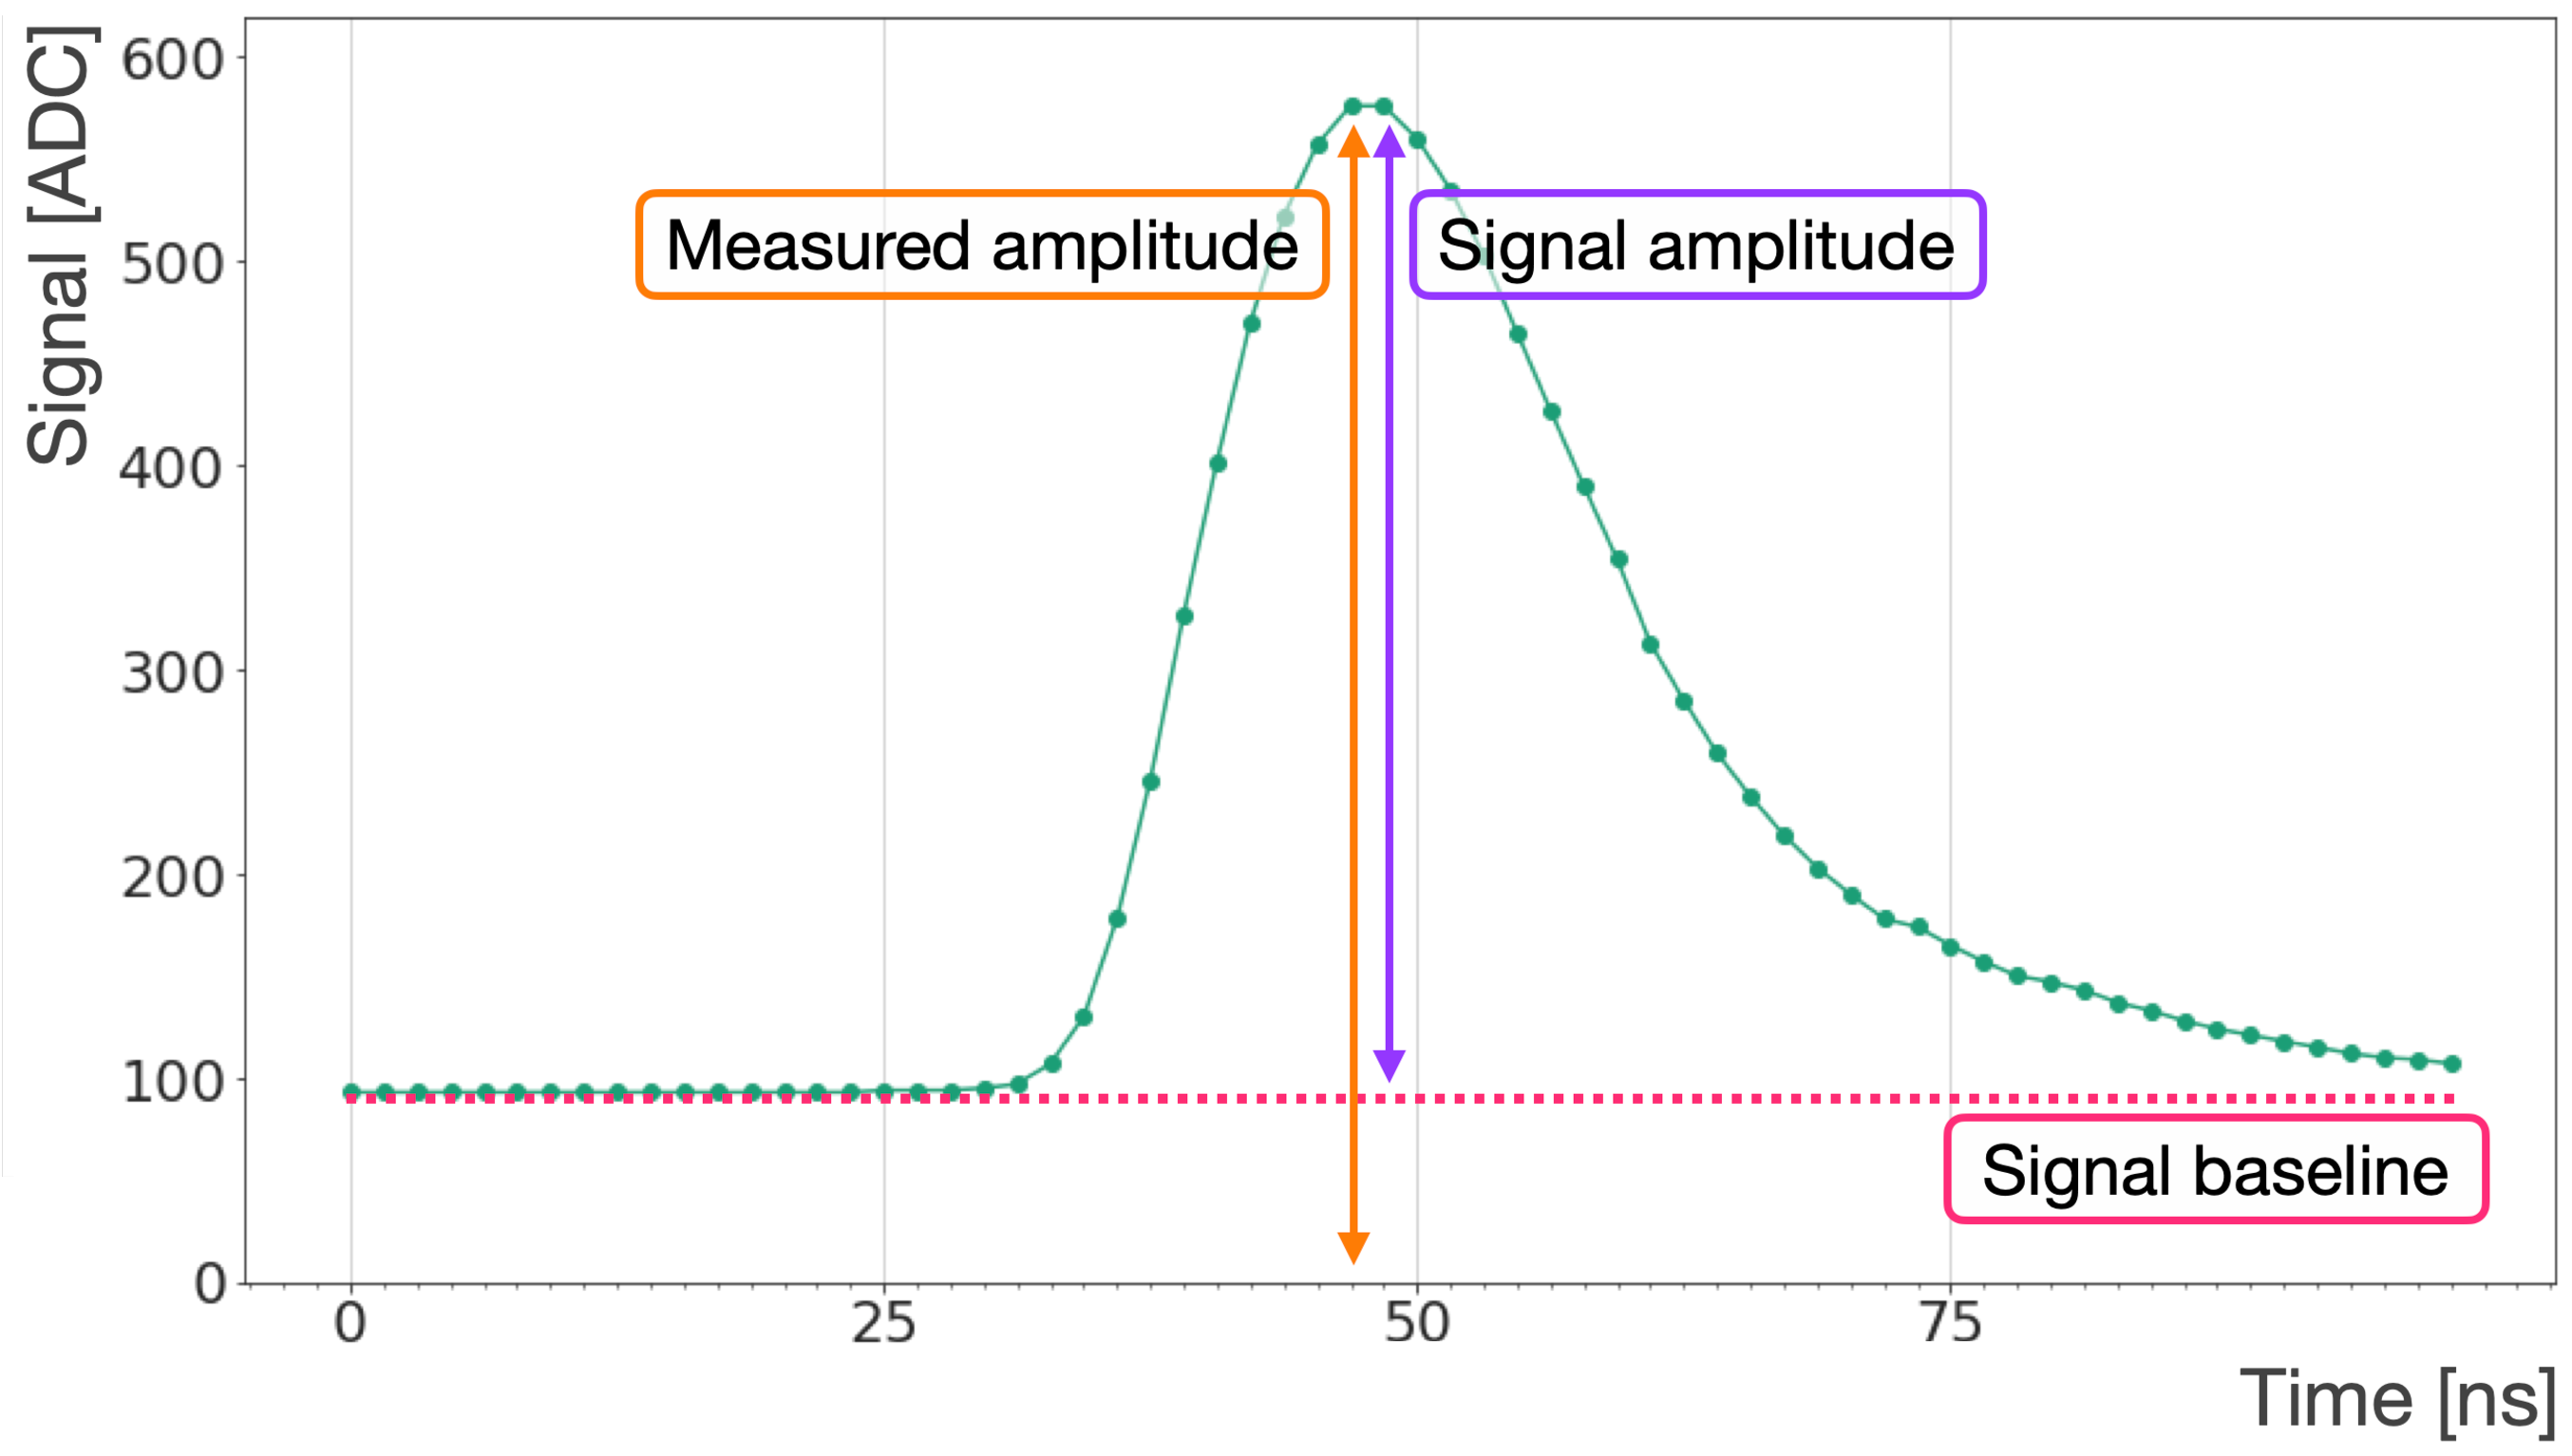
\includegraphics[width=0.5\linewidth]{Figures/HGCAL/SignalBaseline.pdf}
    \caption{A typical signal shape recorder by the HGCROC3: the pink line shows the pedestal baseline. The picture highlights the difference between the measured amplitude (orange) and the real signal amplitude (purple).}
    \label{fig:SignalBaseline}
\end{figure}

The initial step of the chip calibration procedure consists in the tuning of the pedestal values. The pedestal is the baseline of the signal, i.e. the ADC recorded value when no input is present. On the one hand, having a non-zero pedestal is a common practice in electronics devices in order to avoid a possible change in the signal polarisation due to electronic noise or to fluctuations of the ground potential. On the other hand, the pedestal value should be minimised, in order to fully exploit the dynamic range for the measurement of the signal amplitude.
Figure~\ref{fig:SignalBaseline} shows a typical signal shape recorded by the HGCROC3 with a pedestal value around 100~ADC counts. Since every signal is built on top of the baseline, it is important to know the pedestal value and subtract it from the measured amplitude in order to extract the real signal amplitude.

Before the calibration procedure, the 78 independent channels of the HGCROC3 present a large dispersion in their pedestal values, as shown in the left plot of Figure~\ref{fig:Pedestal}. 
A channel-wise parameter (\texttt{Trim\_Inv}) is available in the I2C register to change the pedestal of each channel independently: the parameter is coded into 6 bits, corresponding to 64 possible values.
The \textit{local} per-channel pedestal trimming is performed by scanning all possible values of the parameter and defining as a target the maximum, between all the pedestal values, for a \texttt{Trim\_Inv} value of 0. The \texttt{Trim\_Inv} of each channel will be set to the value giving a pedestal as close as possible to the target.
The full scan of the pedestal trimming value is performed separately for each half of the HGCROC3 and is shown in Figure~\ref{fig:PedestalScan}.

\begin{figure}
    \centering
    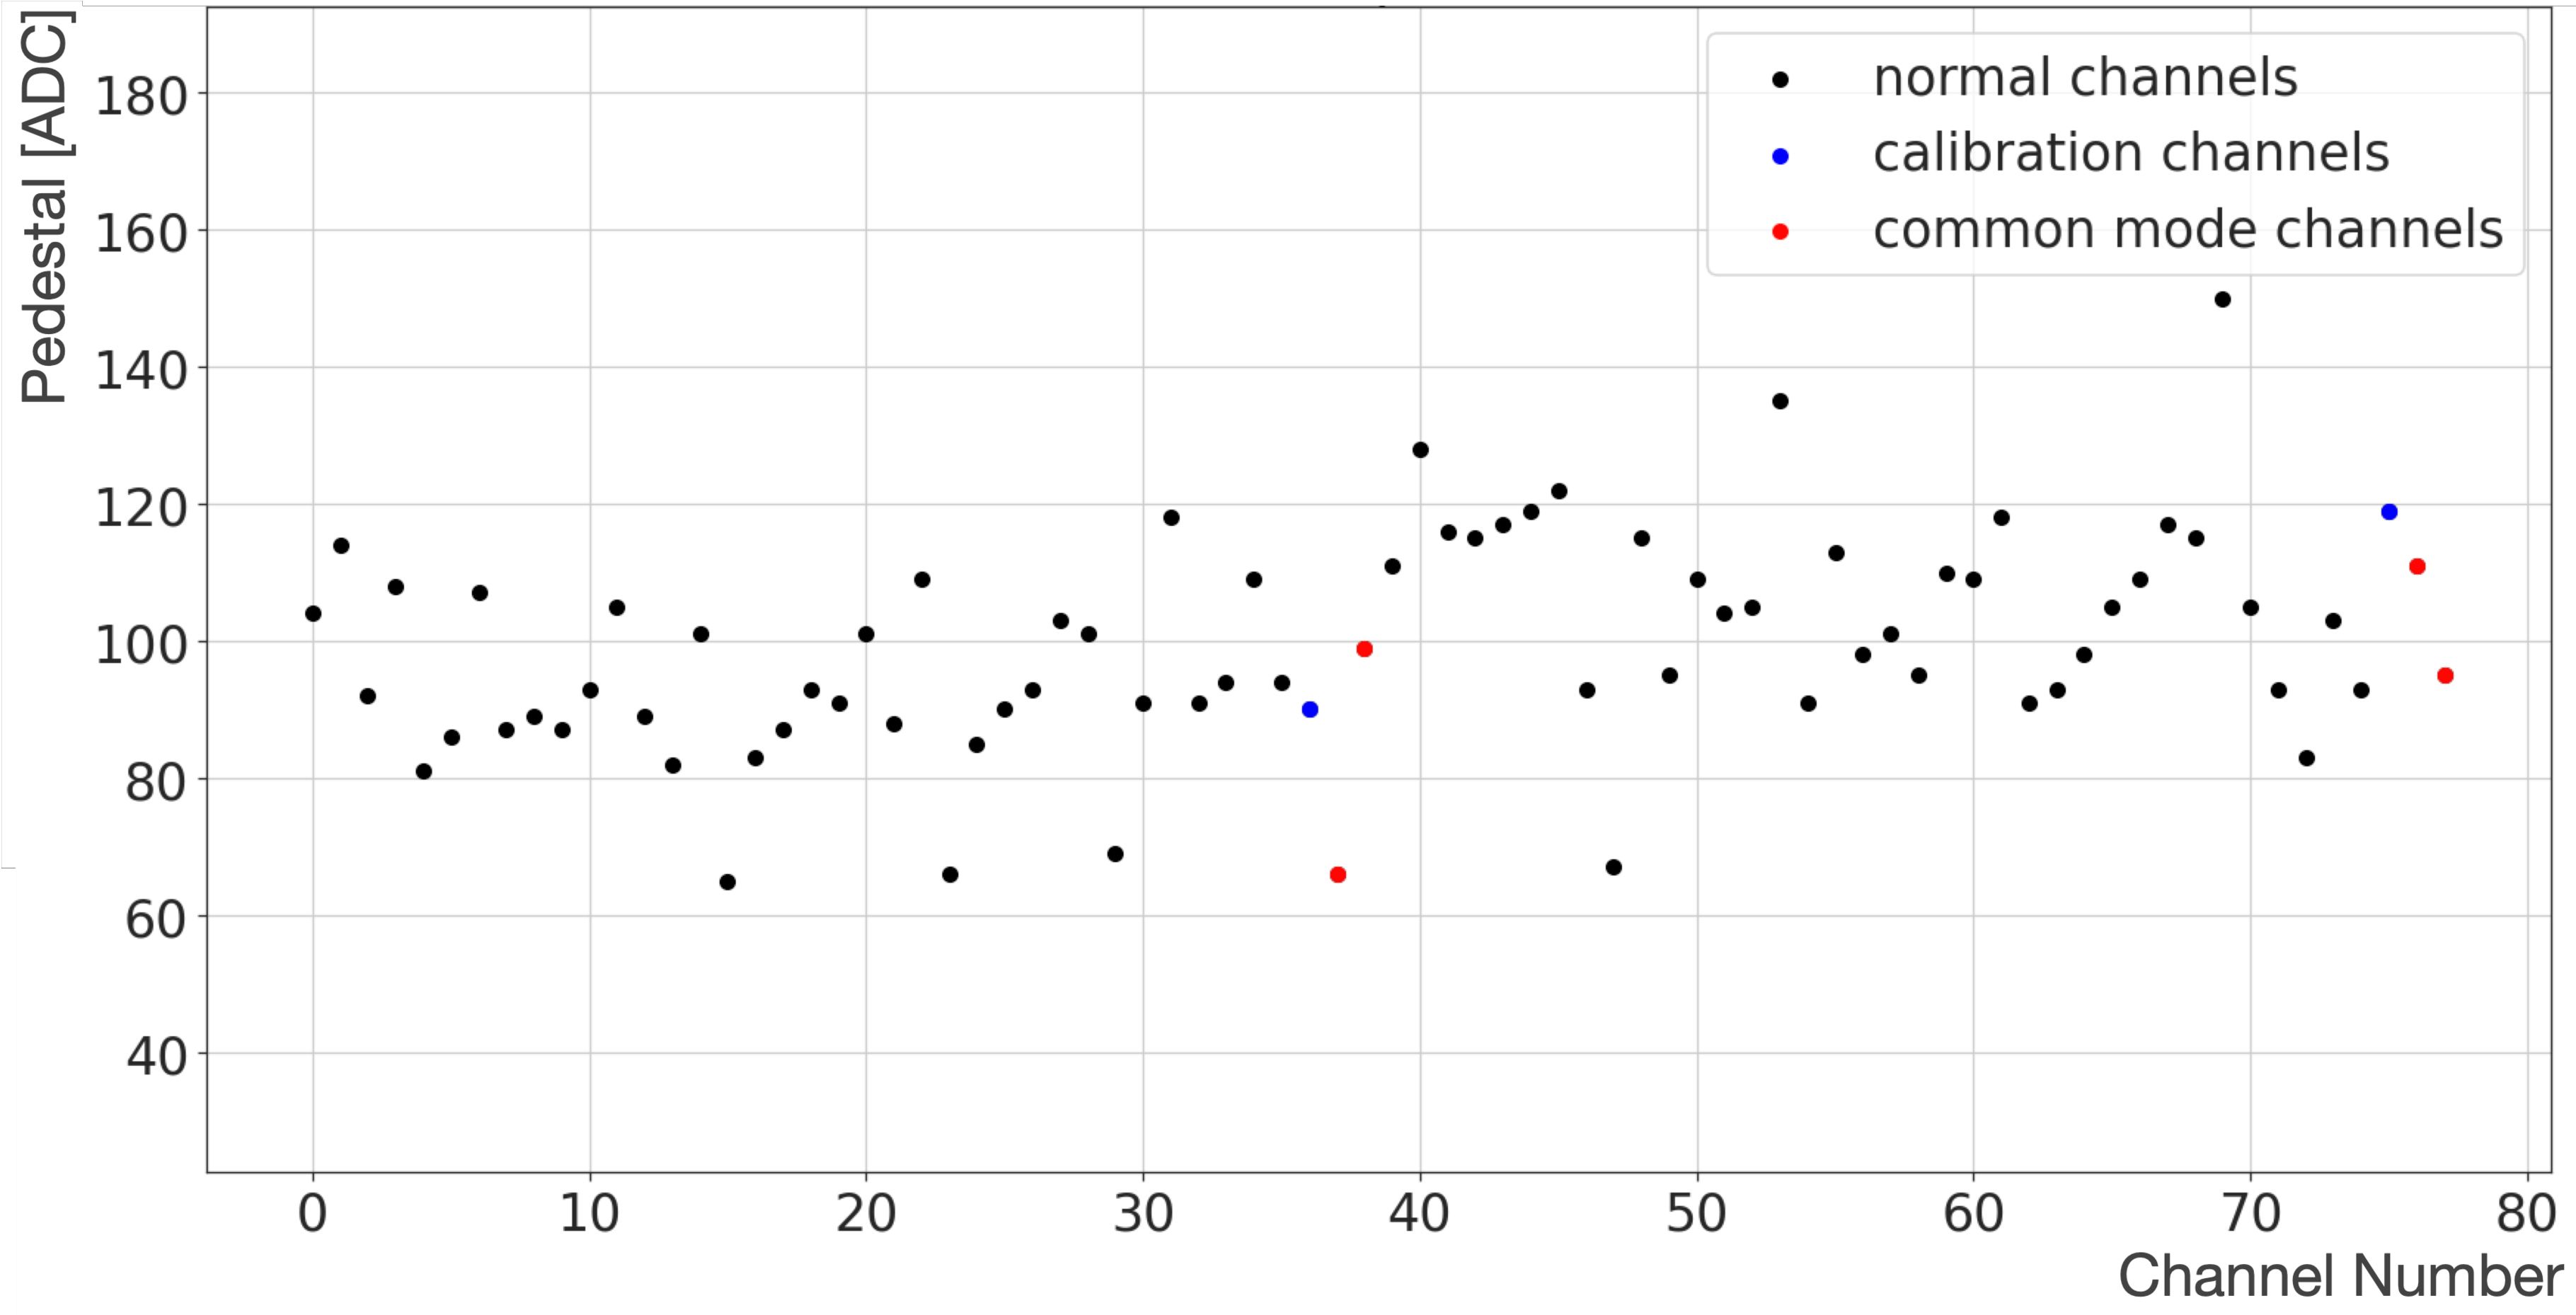
\includegraphics[width=0.49\linewidth]{Figures/HGCAL/Pedestal_0.pdf}
    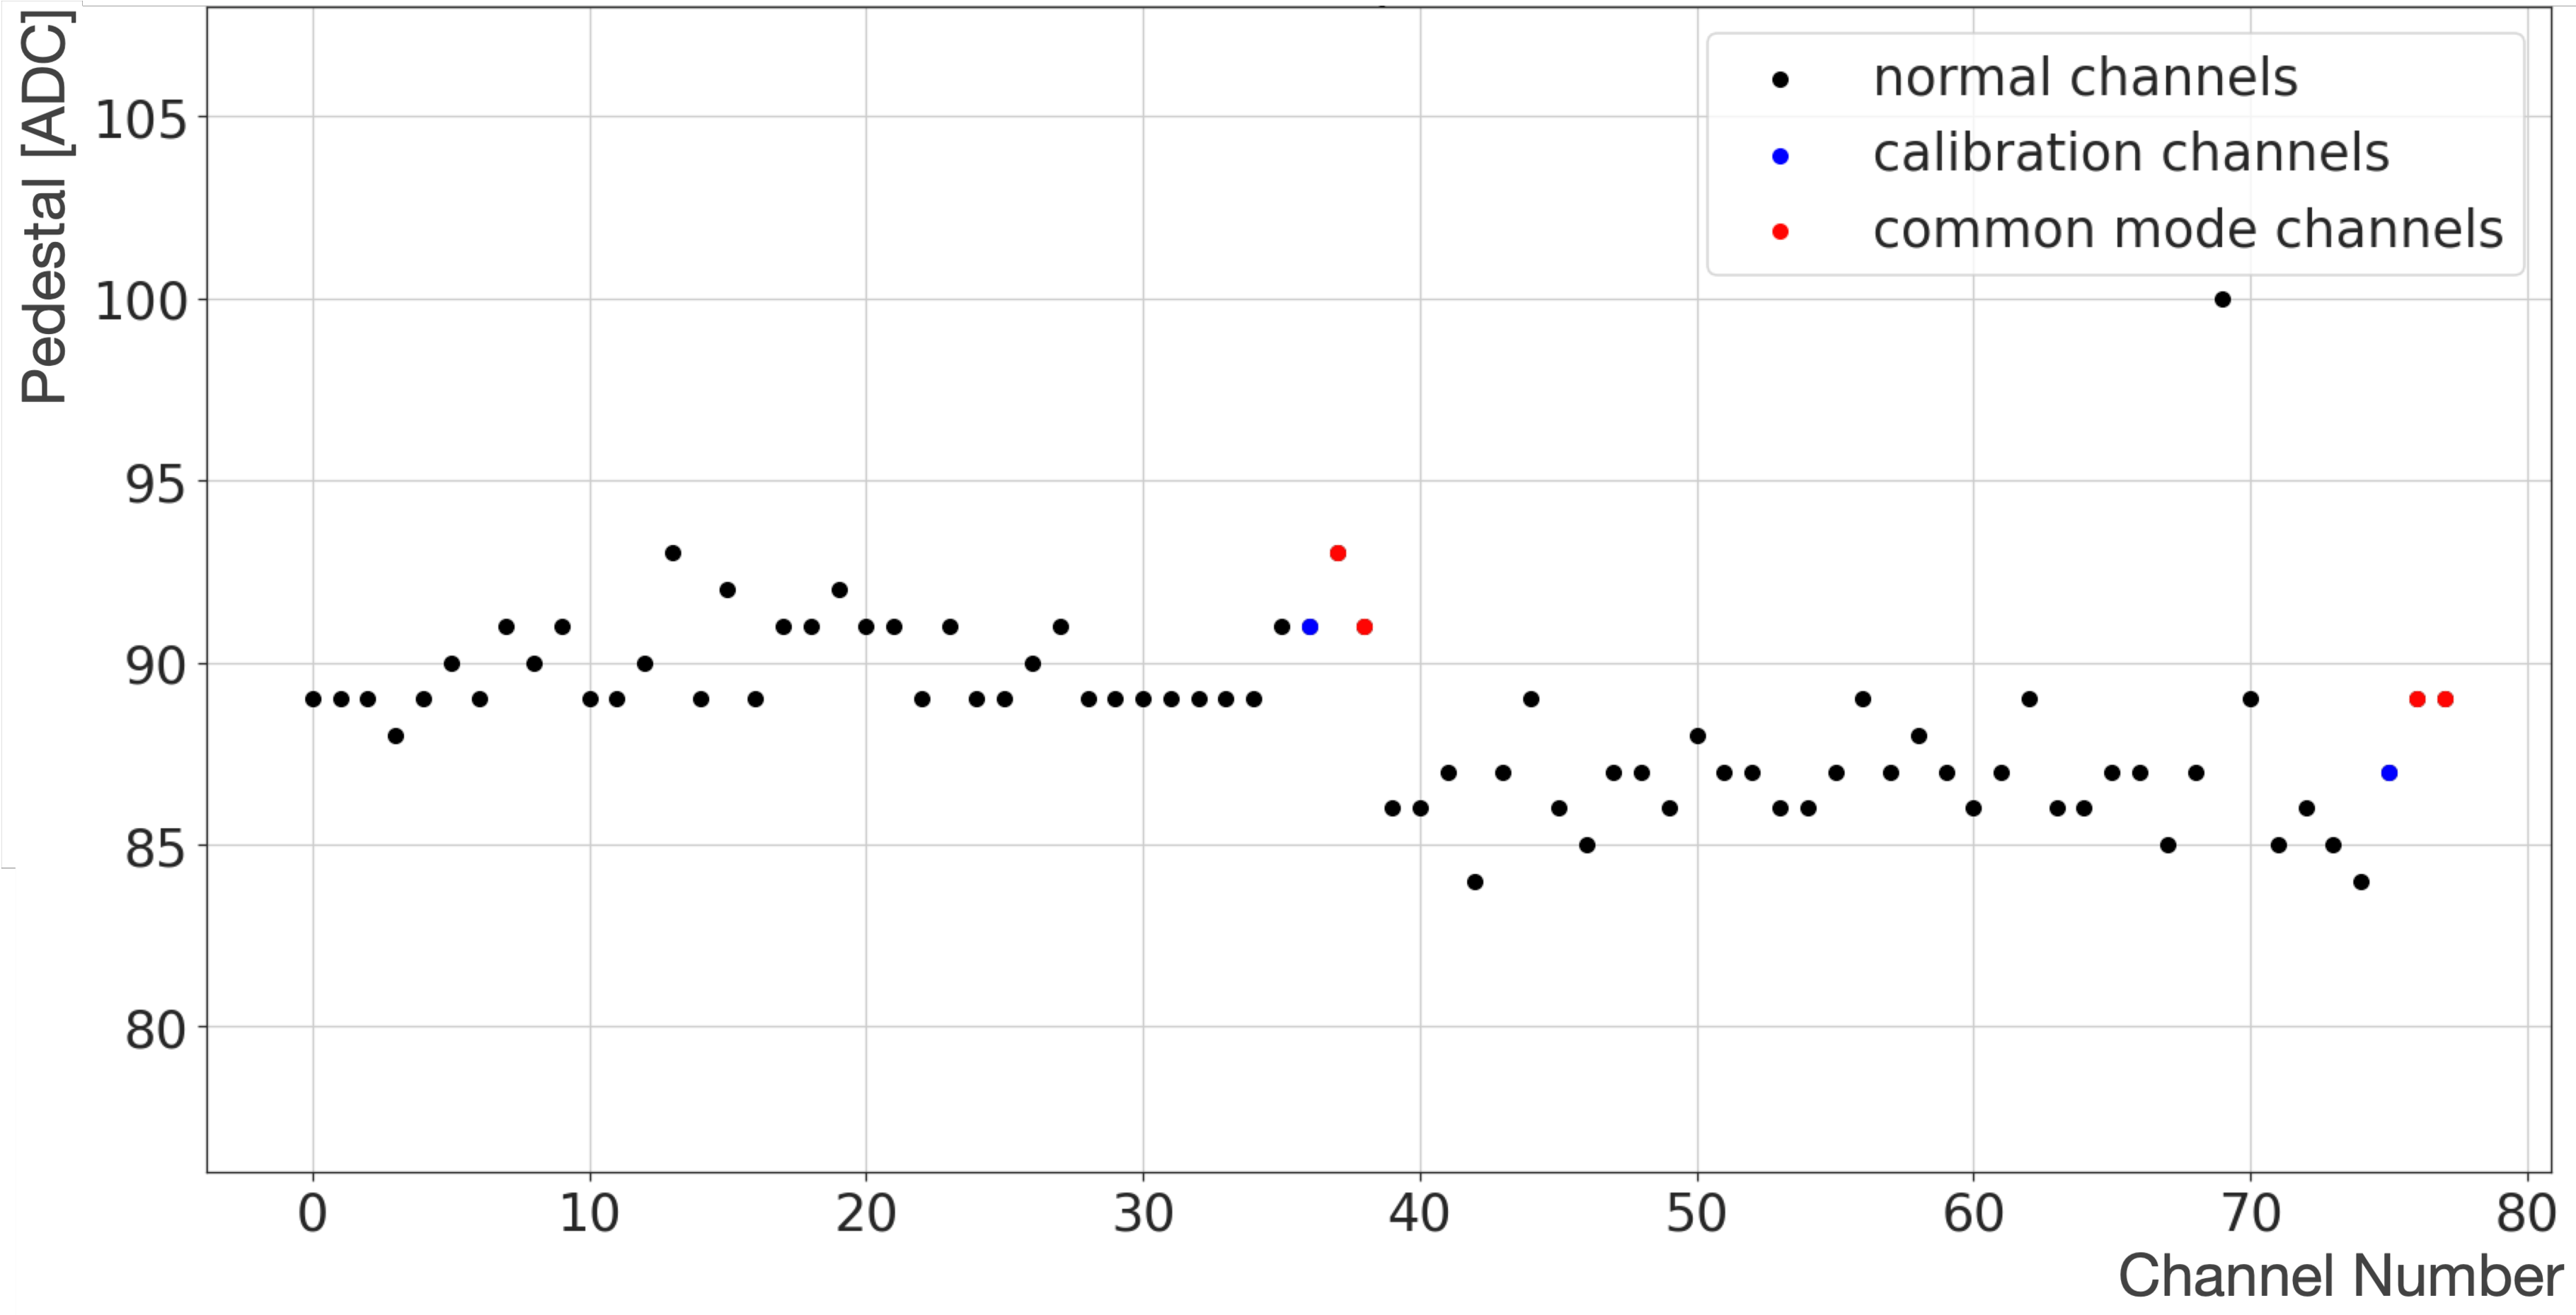
\includegraphics[width=0.49\linewidth]{Figures/HGCAL/Pedestal_1.pdf}
    \caption{Pedestal values of the HGCROC3 channels before (left) and after (right) the pedestal calibration procedure: channel numbers from 0 to 39 belong to the first half, channel numbers from 40 to 77 belong to the second half of the chip. The main target of the calibration is to reduce the dispersion between the channels and minimise their average.}
    \label{fig:Pedestal}
\end{figure}

\begin{figure} 
    \centering
    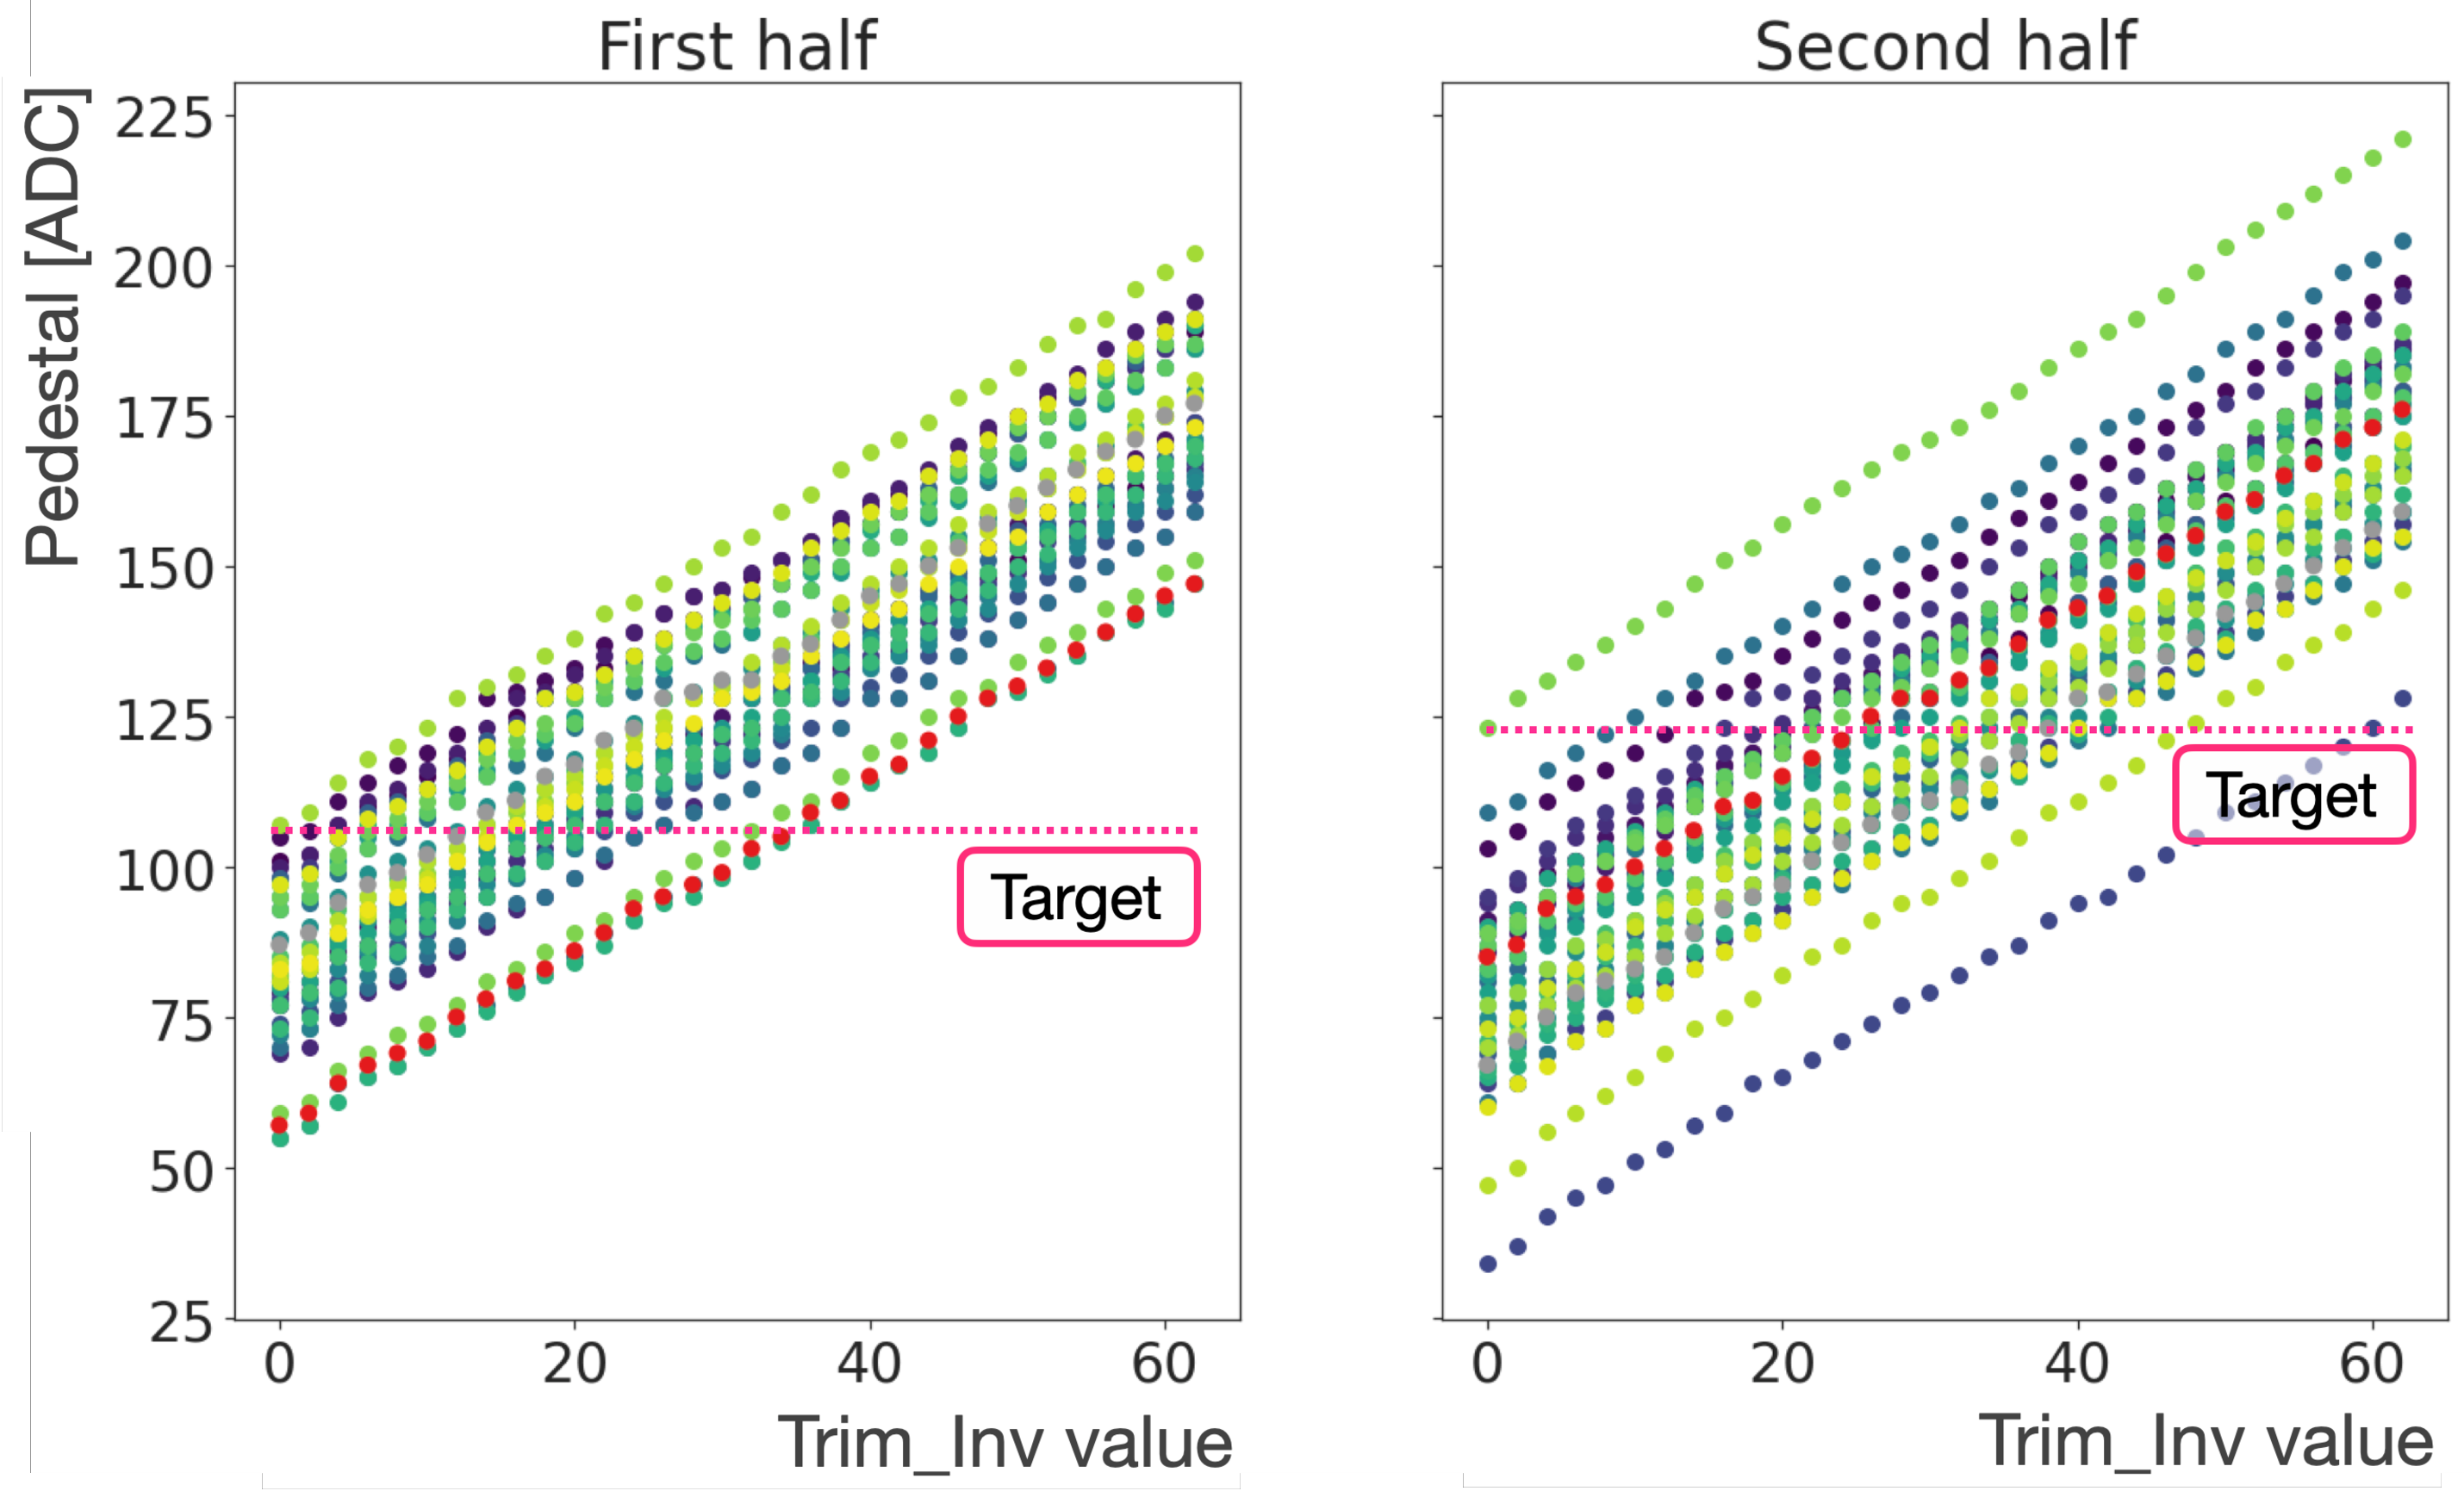
\includegraphics[width=0.7\linewidth]{Figures/HGCAL/PedestalScan.pdf}
    \caption{Pedestal values of the HGCROC3 channels as a function of the \texttt{Trim\_Inv} parameter, used for a channel-wise pedestal trimming.}
    \label{fig:PedestalScan}
\end{figure}

\bigbreak

Once each half shows a similar pedestal value in all channels, a \textit{global} pedestal trimming is performed to lower down the pedestal value to approximately 10~ADC and fully exploit the 1~V digitisation range.
The global pedestal value is configurable through two per-half parameters, \texttt{Vref\_Inv} and \texttt{Vref\_NoInv}, in such a way that the 1~V signal range is placed at the center of the 1.2~V dynamic range of the chip.
The configuration of the pedestal value depends on the expected noise levels and ground fluctuations of testing set-up: in the batch testing experimental conditions, high fluctuations of the ground potential are expected and for this reason the pedestal value is set to a slightly higher level around 50~ADC in order to maintain a discrete margin.

The final configuration of the pedestal values for the 78 channels, after the pedestal calibration procedure is show in the right plot of Figure~\ref{fig:Pedestal}. As a result, also the electronic noise of each channel is reduced after the pedestal calibration, as shown in Figure~\ref{fig:Noise}.

\begin{figure}
    \centering
    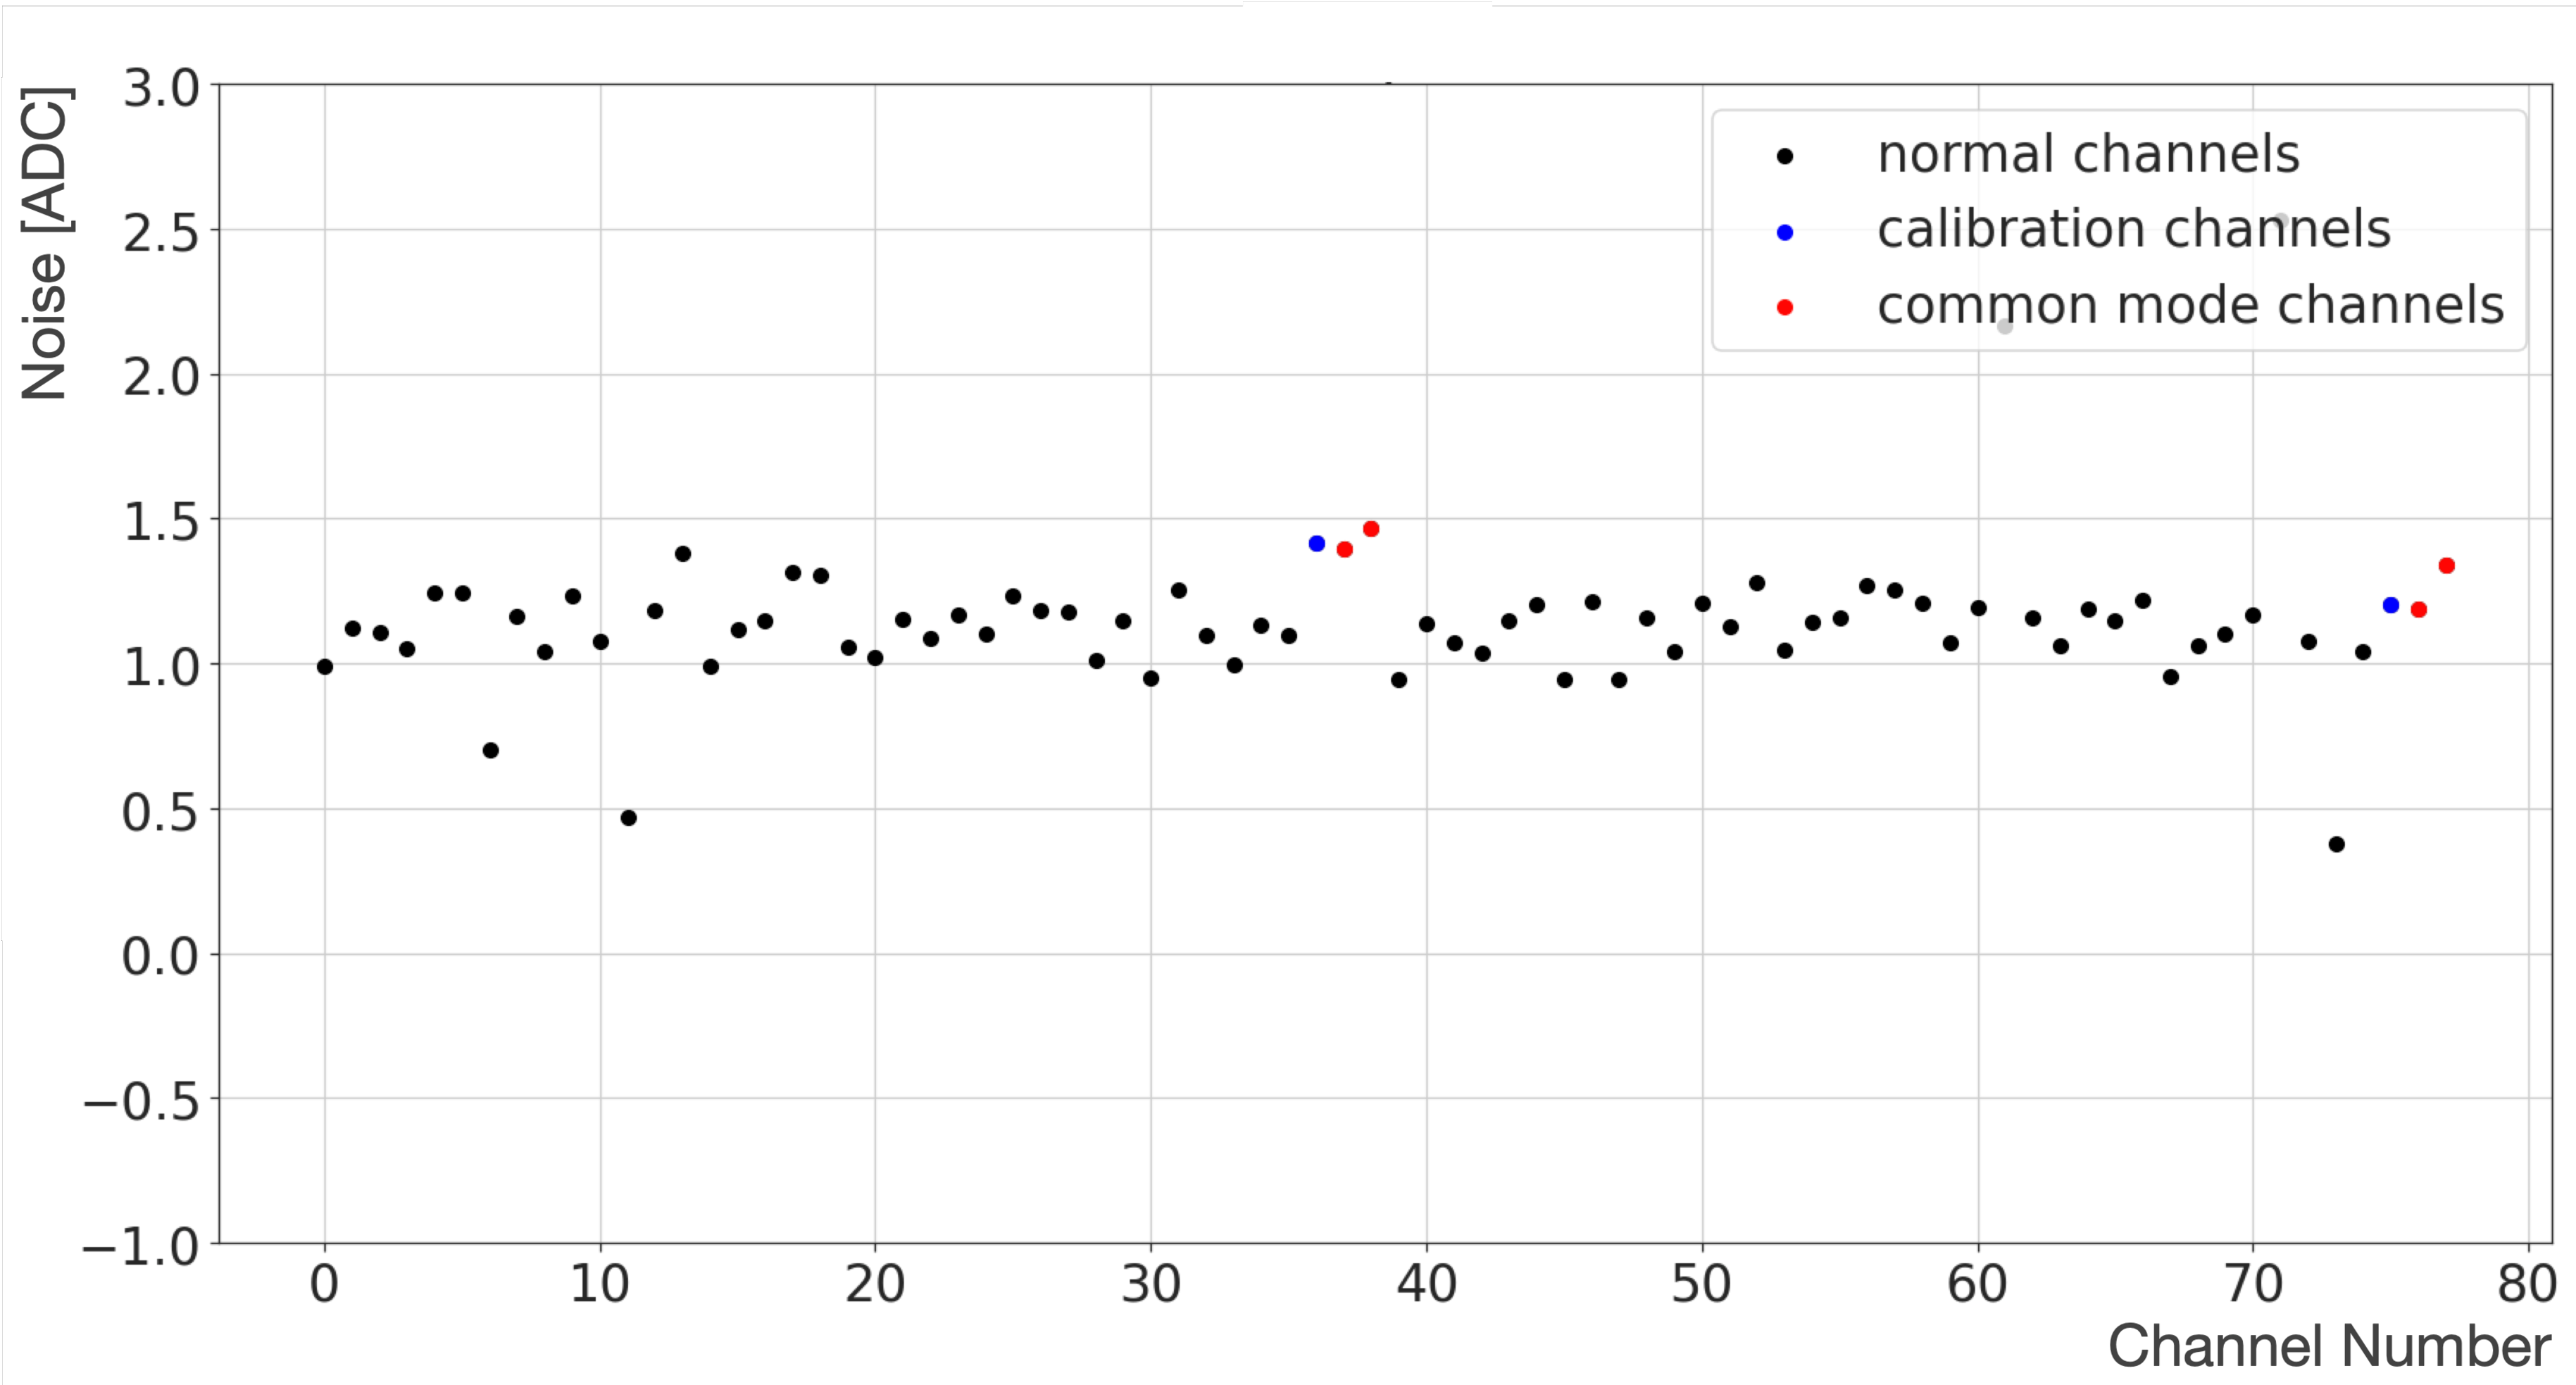
\includegraphics[width=0.49\linewidth]{Figures/HGCAL/Noise_0.pdf}
    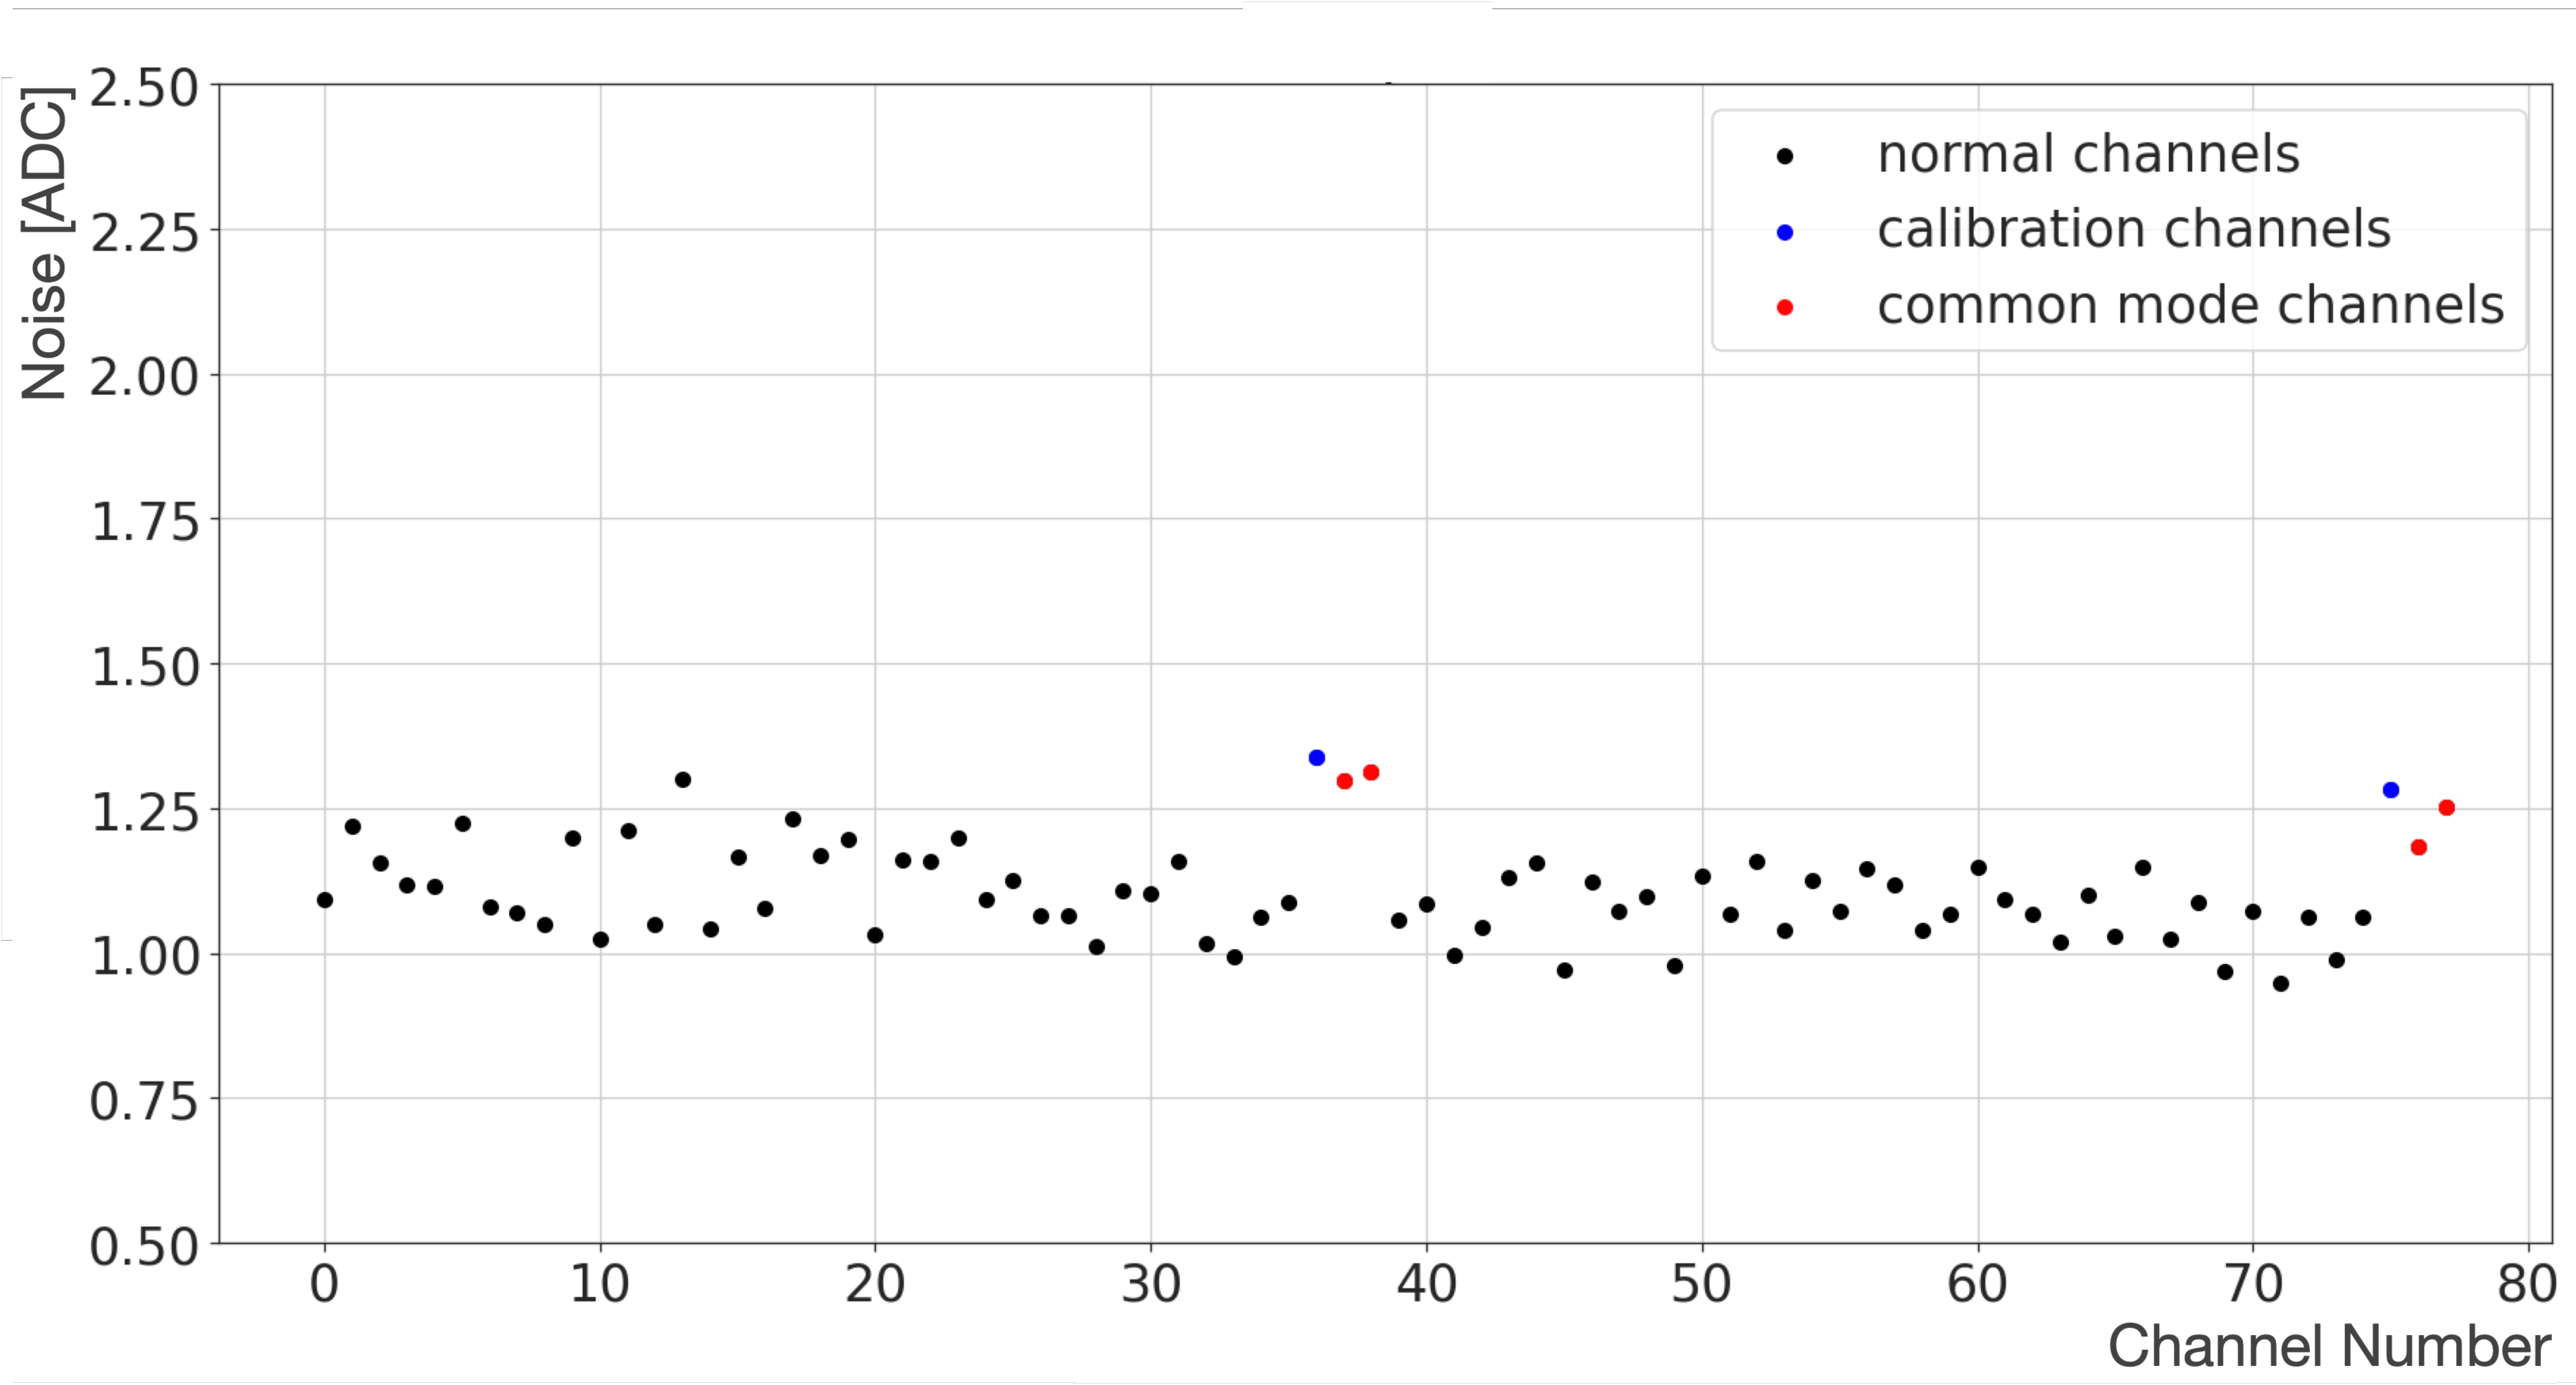
\includegraphics[width=0.49\linewidth]{Figures/HGCAL/Noise_1.pdf}
    \caption{Noise values of the HGCROC3 channels before (left) and after (right) the pedestal calibration procedure: channel numbers from 0 to 39 belong to the first half, channel numbers from 40 to 77 belong to the second half of the chip. The pedestal calibration also aims at minimising the electronic noise of the channels.}
    \label{fig:Noise}
\end{figure}

% Since the analog part of the HGCROC3 is powered at 1.2~V, two per-half parameters are present in the I2C register to place the signal range at the center of the dynamic range.
% In order to better understand this procedure, it is useful to go a bit in the details of the ADC chain. Before the preamplified analog signal enters the ADC block, it is split in two signals with same shape and opposite polarisation: the positively polarised signal enters the \textit{Non Inverted} chain, while the negatively polarised signal enters the \textit{Inverted} chain. Both chains have a 1.2~V dynamic range.
% It is possible to change the values of Vref_inv and Vref_noinv in 10b-DACs (1024 values) to find the best combination. The principle is to force one of the ADC input to 0.6 V (half of the signal range), perform a scan of the Vref DAC of the other branch and set it to the value giving the code 256 ADC (266 in fact to have some margin), and then redo the same operation but for the other branch. By construction, this procedure allows the optimization of both the pedestal and the dynamic range. 

\subsubsection{The time thresholds calibration}
\label{subsubsec:The time thresholds calibration}

The Time-of-Arrival (ToA) denotes the timing measurement of the signal, determined by the moment when the signal amplitude surpasses a predefined threshold value. The ToA threshold should be calibrated slightly above the pedestal level to ensure accurate timing acquisition for the majority of the events. Moreover, the read-out chip should provide the same timing efficiency across different modules and channels, without being affected by fluctuations in the pedestal or noise values.

\bigbreak

In the HGCROC3, two channel-wise parameters (\texttt{ToA\_Vref} and \texttt{Trim\_ToA}) are available to calibrate the ToA thresholds in order to minimise the ToA efficiency dispersion among channels.
For the ToA calibration, a small charge with a fixed ADC amplitude is internally injected into each channel and a scan of different discriminator thresholds is performed. For each threshold, the ToA efficiency is computed, defined as the ratio of ToA triggers to the total number of injected events: if the threshold is low, all events will trigger a ToA signal and the efficiency will be equal to 1, while if the threshold is high, no event will reach the discriminator and the efficiency will be 0.

The ToA efficiency as a function of the different threshold values is presented in the left plot of Figure~\ref{fig:ToAEff} before the calibration procedure.
The goal of the ToA threshold calibration is to have, for a given \texttt{ToA\_Vref} value, the same ToA efficiency in all channels. 
Since the value of the discriminator threshold is defined as the difference between \texttt{ToA\_Vref} and \texttt{Trim\_ToA}, it is possible to configure the channel-wise \texttt{Trim\_ToA} so that the the 50$\%$ efficiency is reached for the same \texttt{ToA\_Vref} value for all channels: the final performance after the calibration procedure is shown in the right plot of Figure~\ref{fig:ToAEff}.

\bigbreak

The Time-over-Threshold (ToT) is a method to provide an estimation of the signal amplitude for very high pulses that saturate the ADC dynamic range by measuring the duration of the signal pulse saturation. 
The ToT is computed only for pulses exceeding the ToT threshold, that needs to be configured below the preamplifier saturation point, in order not to have gaps between the ADC and the ToT dynamic range of measurements. The process of establishing the ToT threshold voltage is similar to the ToA calibration method, and is configurable through equivalent channel-wise parameters, \texttt{ToT\_Vref} and \texttt{Trim\_ToT}.

\begin{figure}
    \centering
    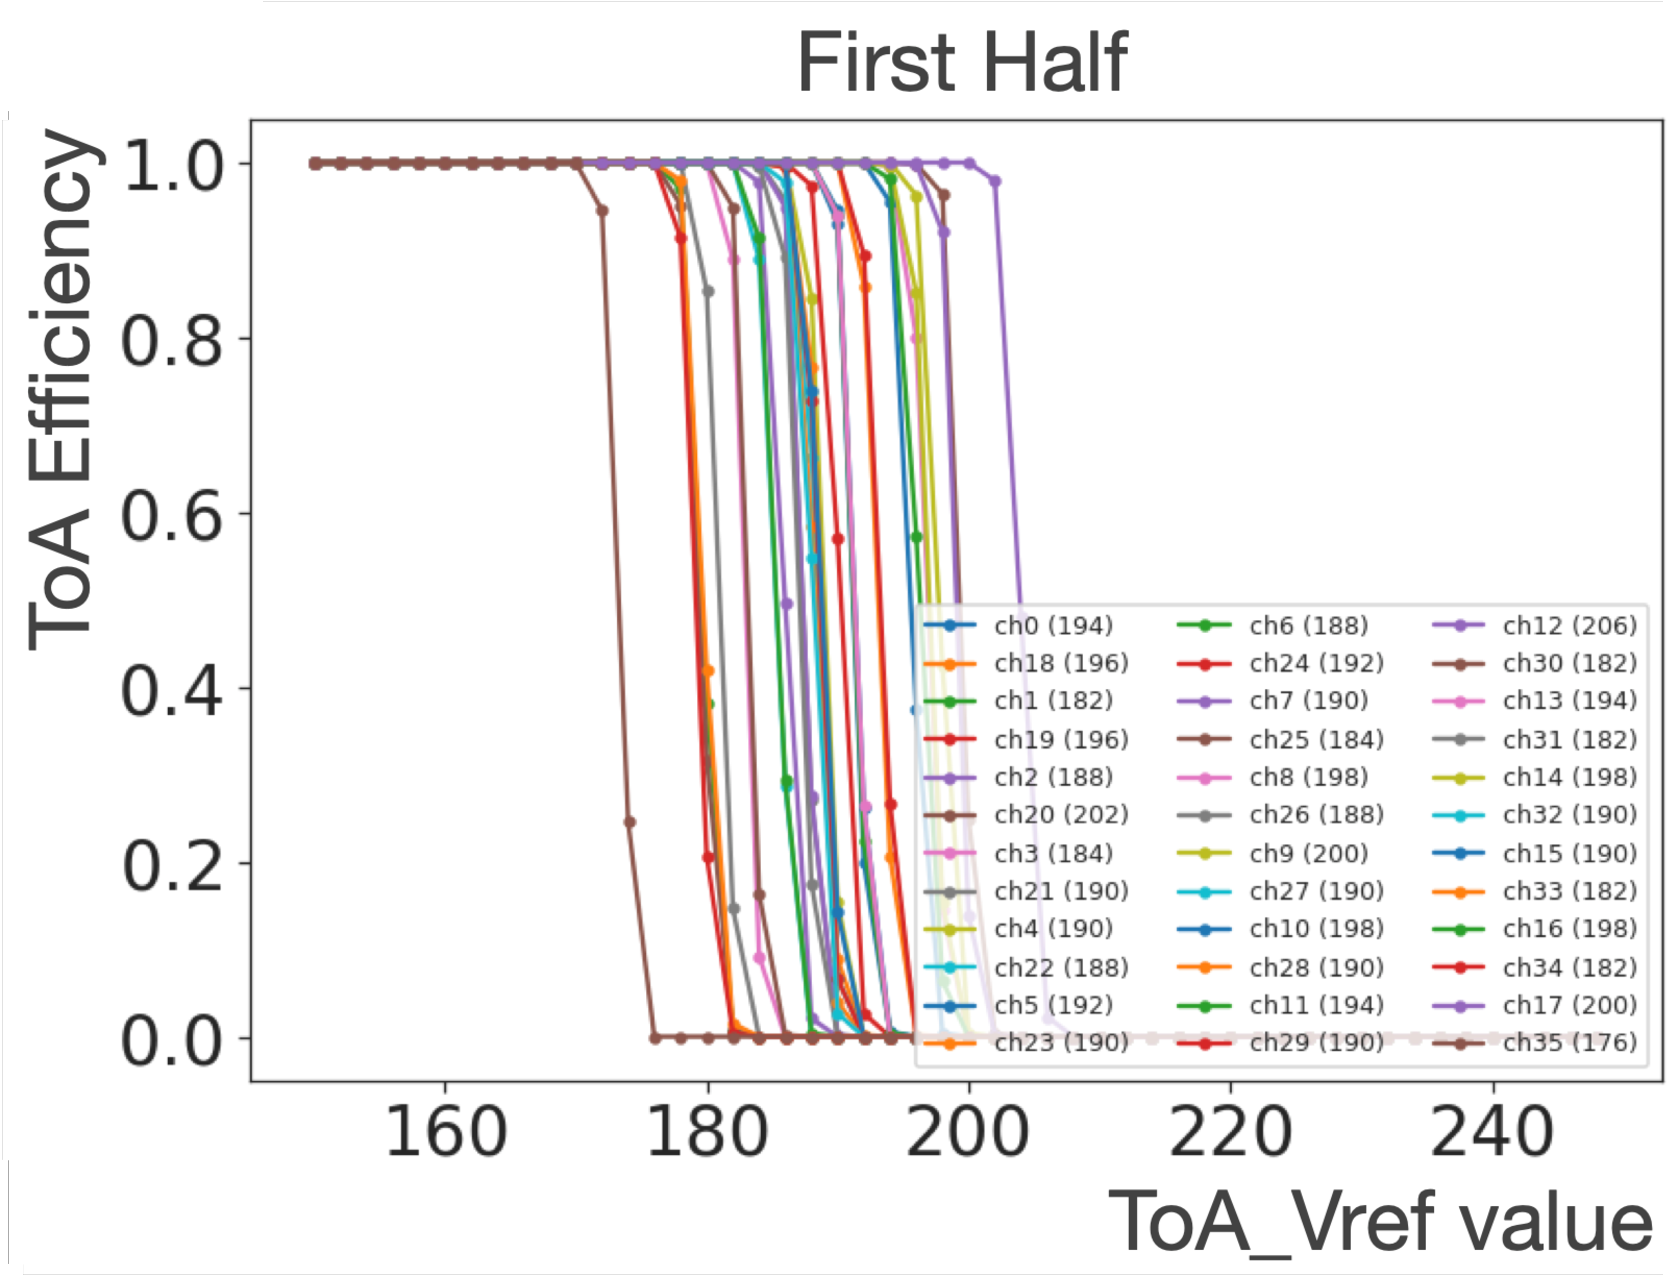
\includegraphics[width=0.49\linewidth]{Figures/HGCAL/ToA_Eff_0.pdf}
    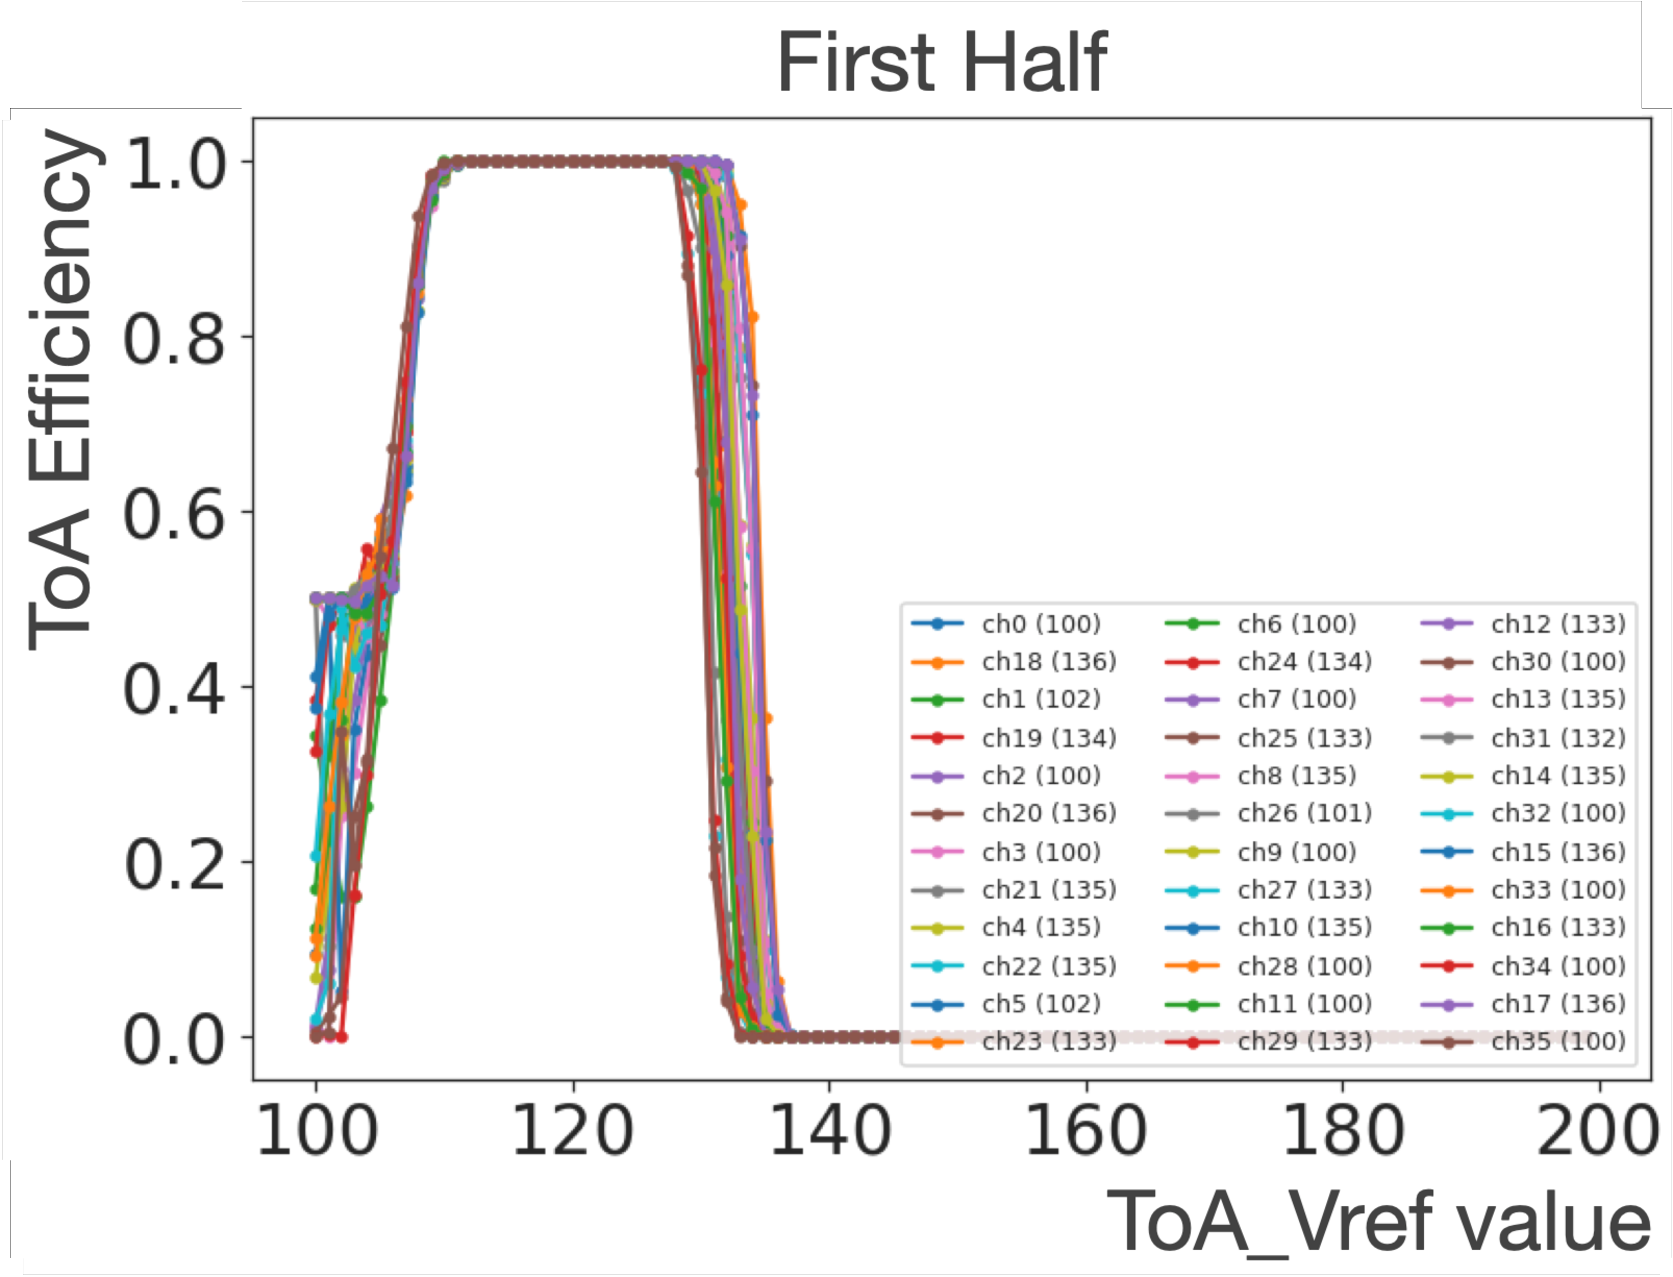
\includegraphics[width=0.49\linewidth]{Figures/HGCAL/ToA_Eff_1.pdf}
    \caption{ToA efficiency, defined as the ratio between ToA triggered events and total number of injected events, as a function of the \texttt{ToA\_Vref} parameter, defining the ToA discriminator threshold, before (left) and after (right) the ToA threshold calibration procedure.}
    \label{fig:ToAEff}
\end{figure}

% The ToA injection scan measures the time of arrival of the signal. The ToA is the instant of time at which the signal amplitude exceeds a threshold value. You can see from the example that a smaller signal amplitude provides a bigger ToA, while a higher signal amplitude leads to a smaller ToA. This is reflected in the right plot, where we can see the so-called “time walk”.

\subsubsection{The phase calibration}
\label{subsubsec:The phase calibration}

In order to correctly measure the amplitude of the physical signal, the ADC and TDC conversion blocks of the HGCROC3 are provided with an adjustable sampling phase parameter.
Each 25~ns bunch crossing (BX) period is internally sampled into 16 phases: each ASIC can be configured in such a way that the signal amplitude is sampled at the correct phase, which might depend on the rapidity angle of the module and on the silicon sensor thickness.

Figure~\ref{fig:BestPhase} shows a scan over phases of the ADC value that reconstructs the signal shape of an injected pulse: in this case, the sampling phase corresponding to the signal peak is determined to be phase 0.
The signal sampling also shows an oscillation in the pedestal value, due to the fluctuation of the ground potential, that can be subtracted through the common mode channels.

\begin{figure}[b!]
    \centering
    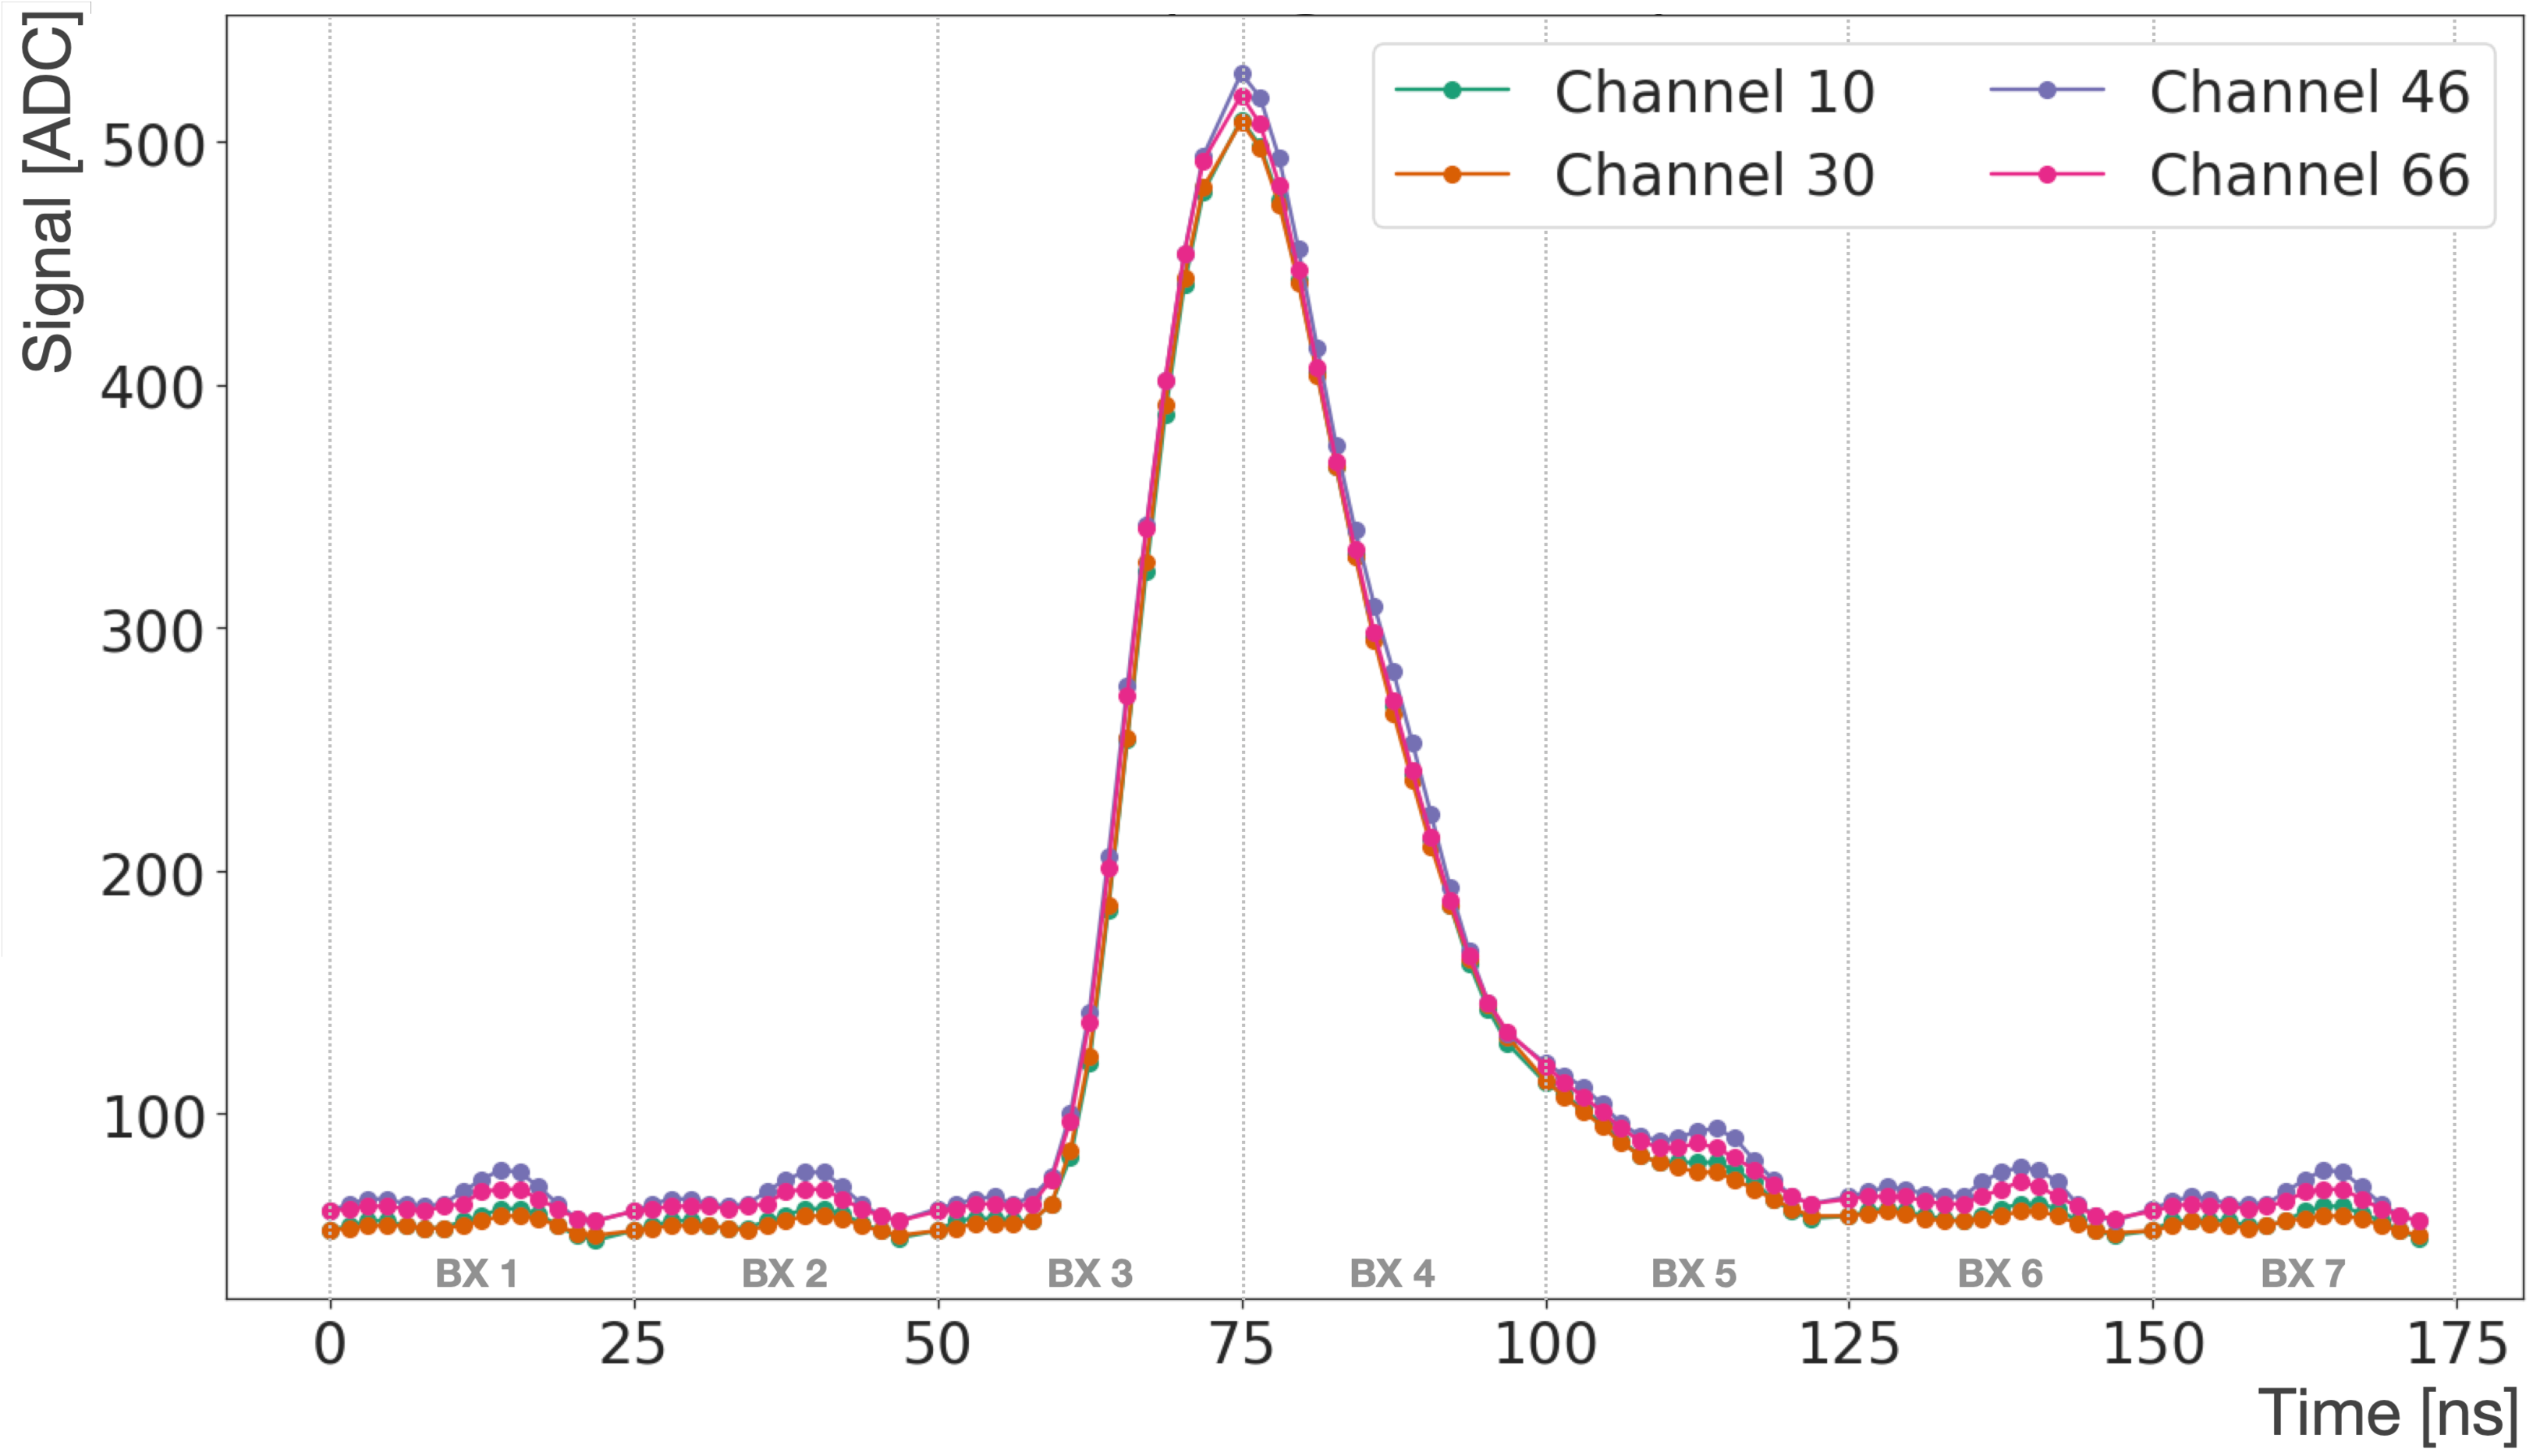
\includegraphics[width=0.65\linewidth]{Figures/HGCAL/BestPhase.pdf}
    \caption{Sampling scan of the ADC value of 4 channels for different phases. Each 25~ns bunch crossing (BX) period is divided into 16 phases: the sampling position is determined by the phase of the signal maximum.}
    \label{fig:BestPhase}
\end{figure}

\bigbreak

Other configurable parameters exist within the HGCROC3 I2C register, but are not addressed in this context as they are not relevant for the discussion.

\subsection{The HGCROC3 performance}
\label{subsec:The HGCROC3 performance}

Once the HGCROC3 is correctly configured for the data acquisition, it's possible to test its performance.
The ASIC can measure charges spanning from 160~fC to 320~pC, with two different regimes: the ADC is calibrated to accurately detect charges up to the preamplifier saturation, when the saturation is reached the Time-Over-Threshold (ToT) technique measures the signal duration during saturation. The transition from ADC to ToT is configurable through the chip parameters. The preamplifier output is also connected to the Time-Of-Arrival (ToA) discriminator to capture timing information. 

Considering the different types of signal pulses to be read out by the HGCROC2, it is essential to evaluate the response of the device to different signal pulses in terms of ADC, ToA and ToT.

\subsubsection{The ADC performance}
\label{subsubsec:The ADC performance}

The front-end ADC operates at 40 MHz to convert the analog signal into a digitised value corresponding to the signal amplitude and consequently to energy deposit in the detector. 
Figure~\ref{fig:FitSampling} shows a typical signal pulse recorder by the HGCROC3 and fitted using Equation~\ref{eq:FitSampling}. The model well describes the recorded data, with minor discrepancies below 2\%.

\begin{equation}
    f(t) = A_{0}\,e^{-at}\left[e^{-ct}\left(\frac{t^3}{c}-\frac{3t^2}{c^2}+\frac{6t}{c^3}-\frac{6}{c^4}\right)+\frac{6}{c^4}\right], \;\; a =\frac{1}{\tau_{p}}, \;\; c=\frac{1}{\tau_{p}}-\frac{1}{\tau_{s}}
\label{eq:FitSampling}
\end{equation}

\begin{figure}
    \centering
    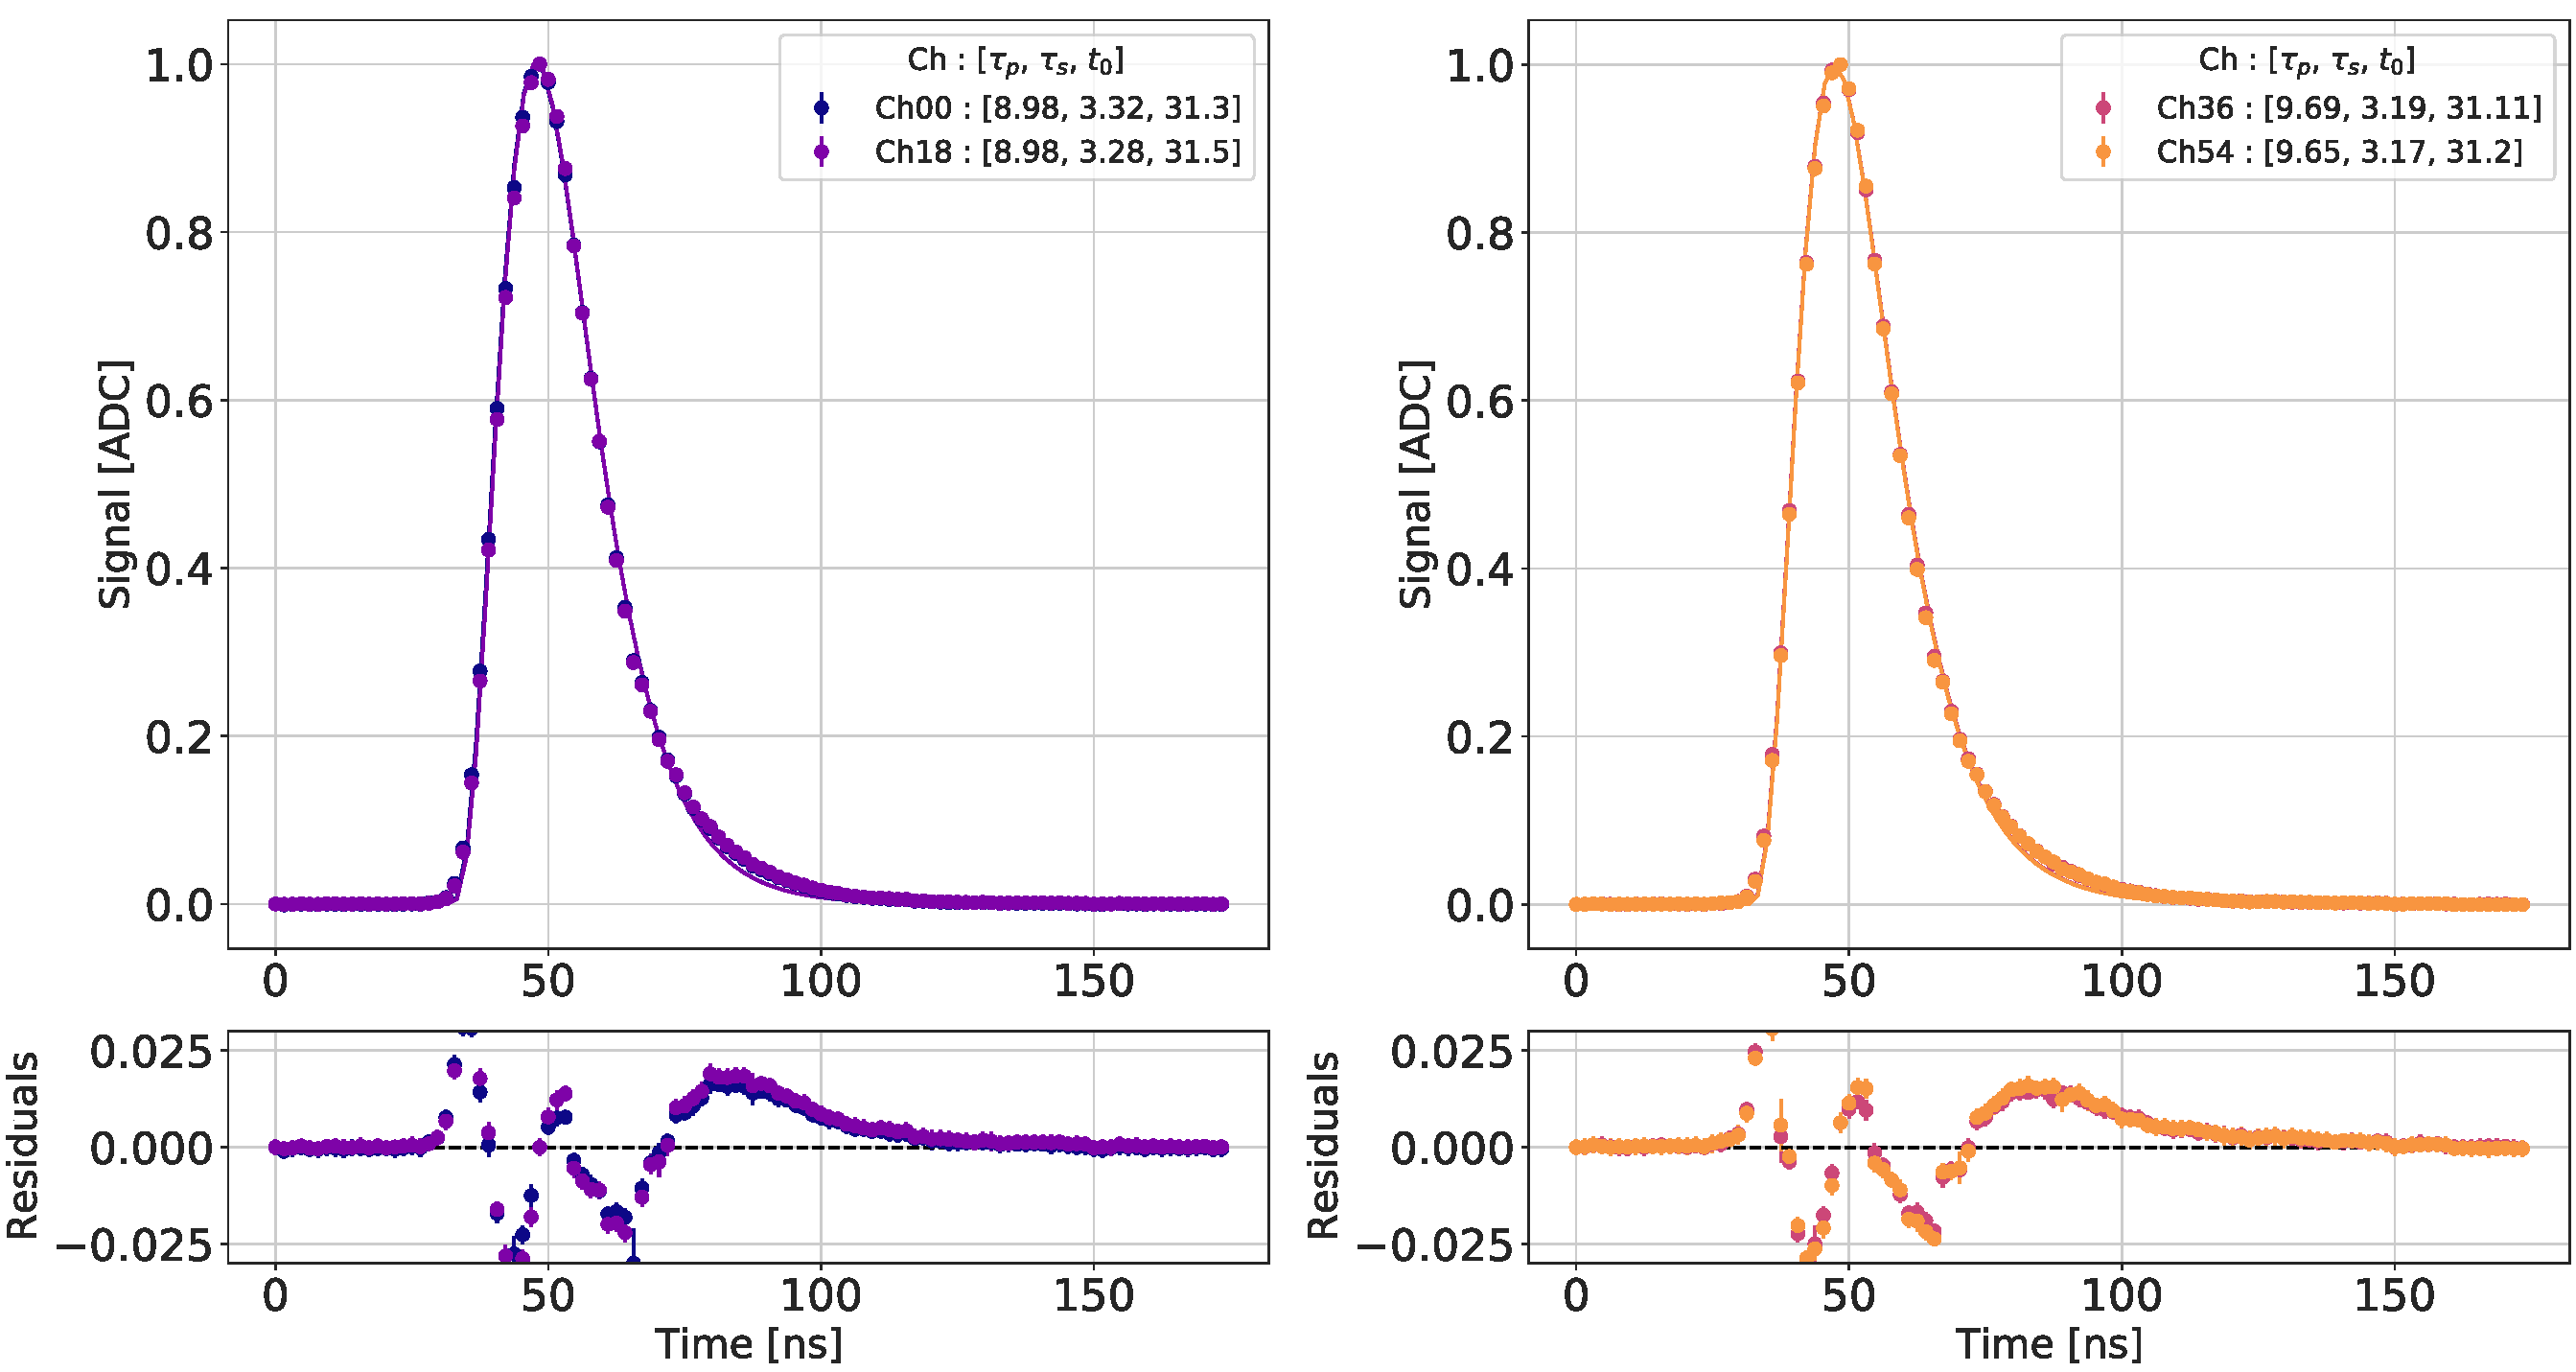
\includegraphics[width=0.75\linewidth]{Figures/HGCAL/FitSampling.pdf}
    \caption{Normalised signal pulse for 4 channels of the HGCROC3, two channels of the first half (left) and two channels of the second half (right). The signal shape is fitted using Equation~\ref{eq:FitSampling} and the optimised parameters of the fit are reported in the legend. Discrepancies between the model and the data are below 2\%.}
    \label{fig:FitSampling}
\end{figure}

A high linearity is crucial for the ADC to accurately measure the signal peak and ensure precise charge measurements. The ADC performance is tested by injecting signals with increasing charge value and verifying the linearity of the recorded ADC as a function of the input charge. Figure~\ref{fig:ADC_Injection} shows the expected linear response of the signal amplitude measured by the HGCROC3 with respect to the injected charge, in units of the \texttt{Calib\_DAC} parameter - a \texttt{Calib\_DAC} value of 4096 corresponds to a charge of 500~fC. The linear function described in Equation~\ref{eq:ADCLinearity} is used to test the linearity of the response.

\begin{equation}
    f(t) = ax + b
\label{eq:ADCLinearity}
\end{equation}

\begin{figure}
    \centering
    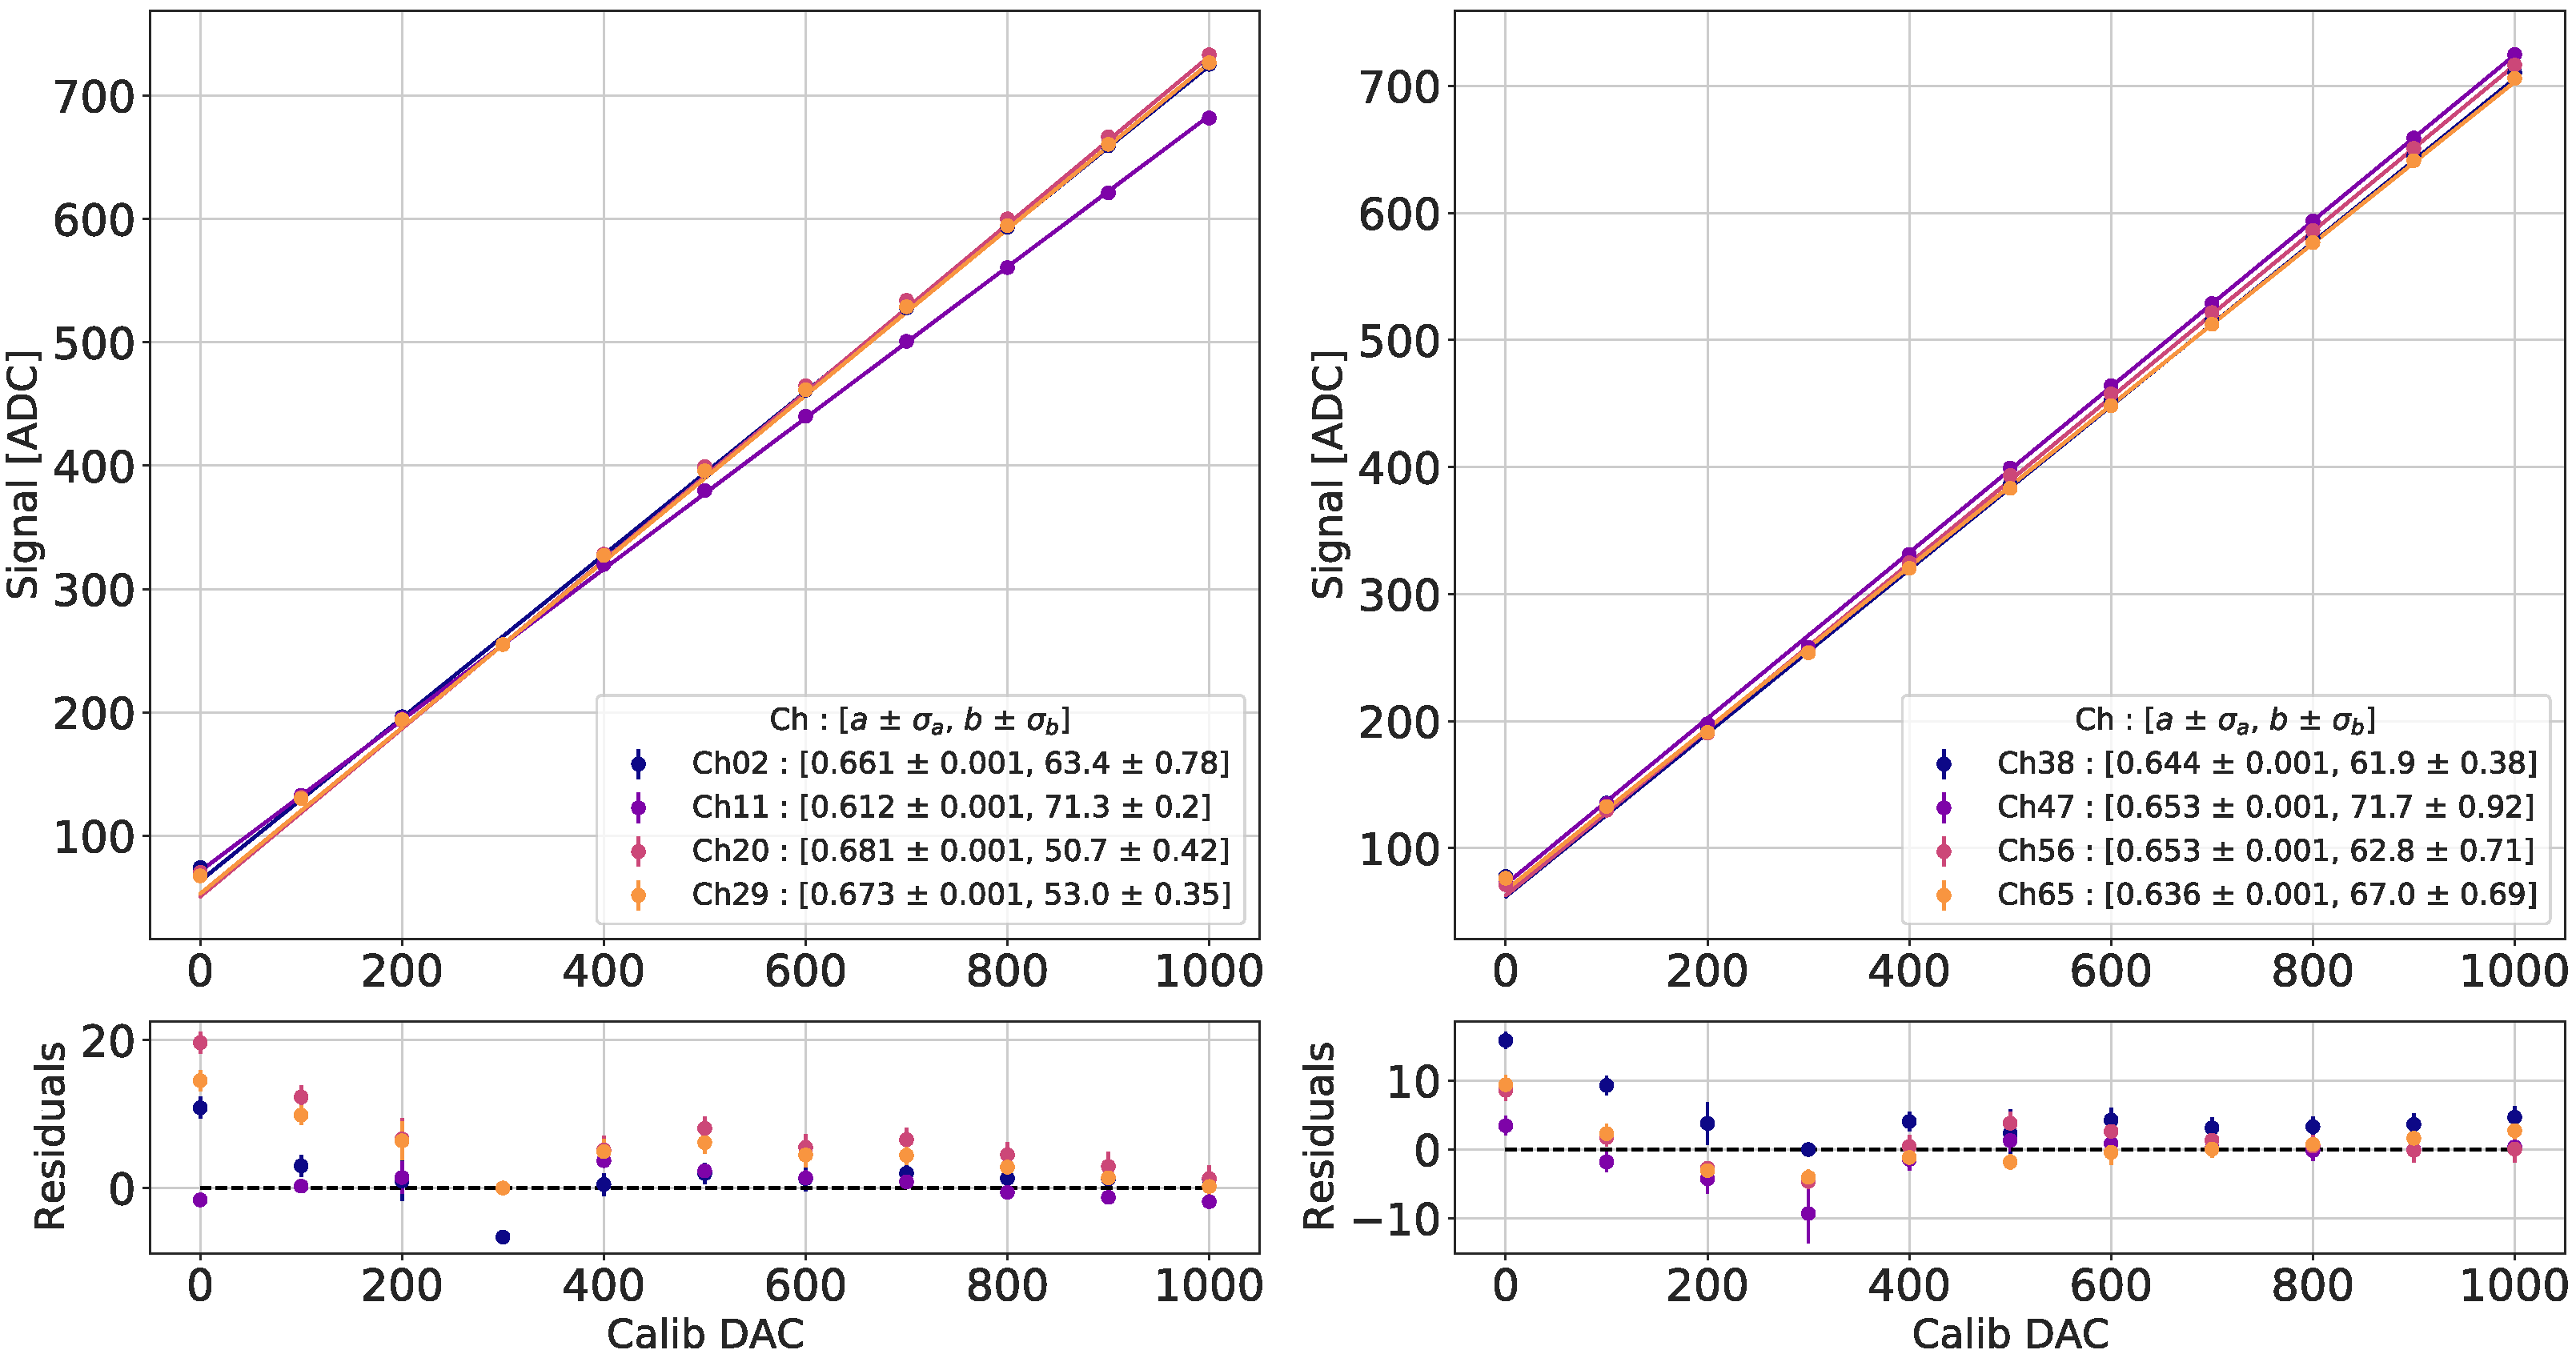
\includegraphics[width=0.75\linewidth]{Figures/HGCAL/ADC_Injection.pdf}
    \caption{The ADC response linearity to multiple injections corresponding to different \texttt{Calib\_DAC} values, defining the input charge. The  response is fitted with the linear function in Equation~\ref{eq:ADCLinearity} and the optimised parameters of the fit are reported in the legend.}
    \label{fig:ADC_Injection}
\end{figure}

\subsubsection{The ToT performance}
\label{subsubsec:The ToT performance}

When the preamplifier enters the saturation region, the signal duration becomes proportional to the injected charge. 
The Time-over-Threshold (ToT) technique measures the time difference between the start and the end of the saturation time. Figure~\ref{fig:TOT_Injection} illustrates the ToT measurements for different injected charges. The ToT curve is fitted by using Equation~\ref{eq:ADCLinearity} and the performance shows a good linearity up to the highest charge of 500~fC. 

\begin{figure}
    \centering
    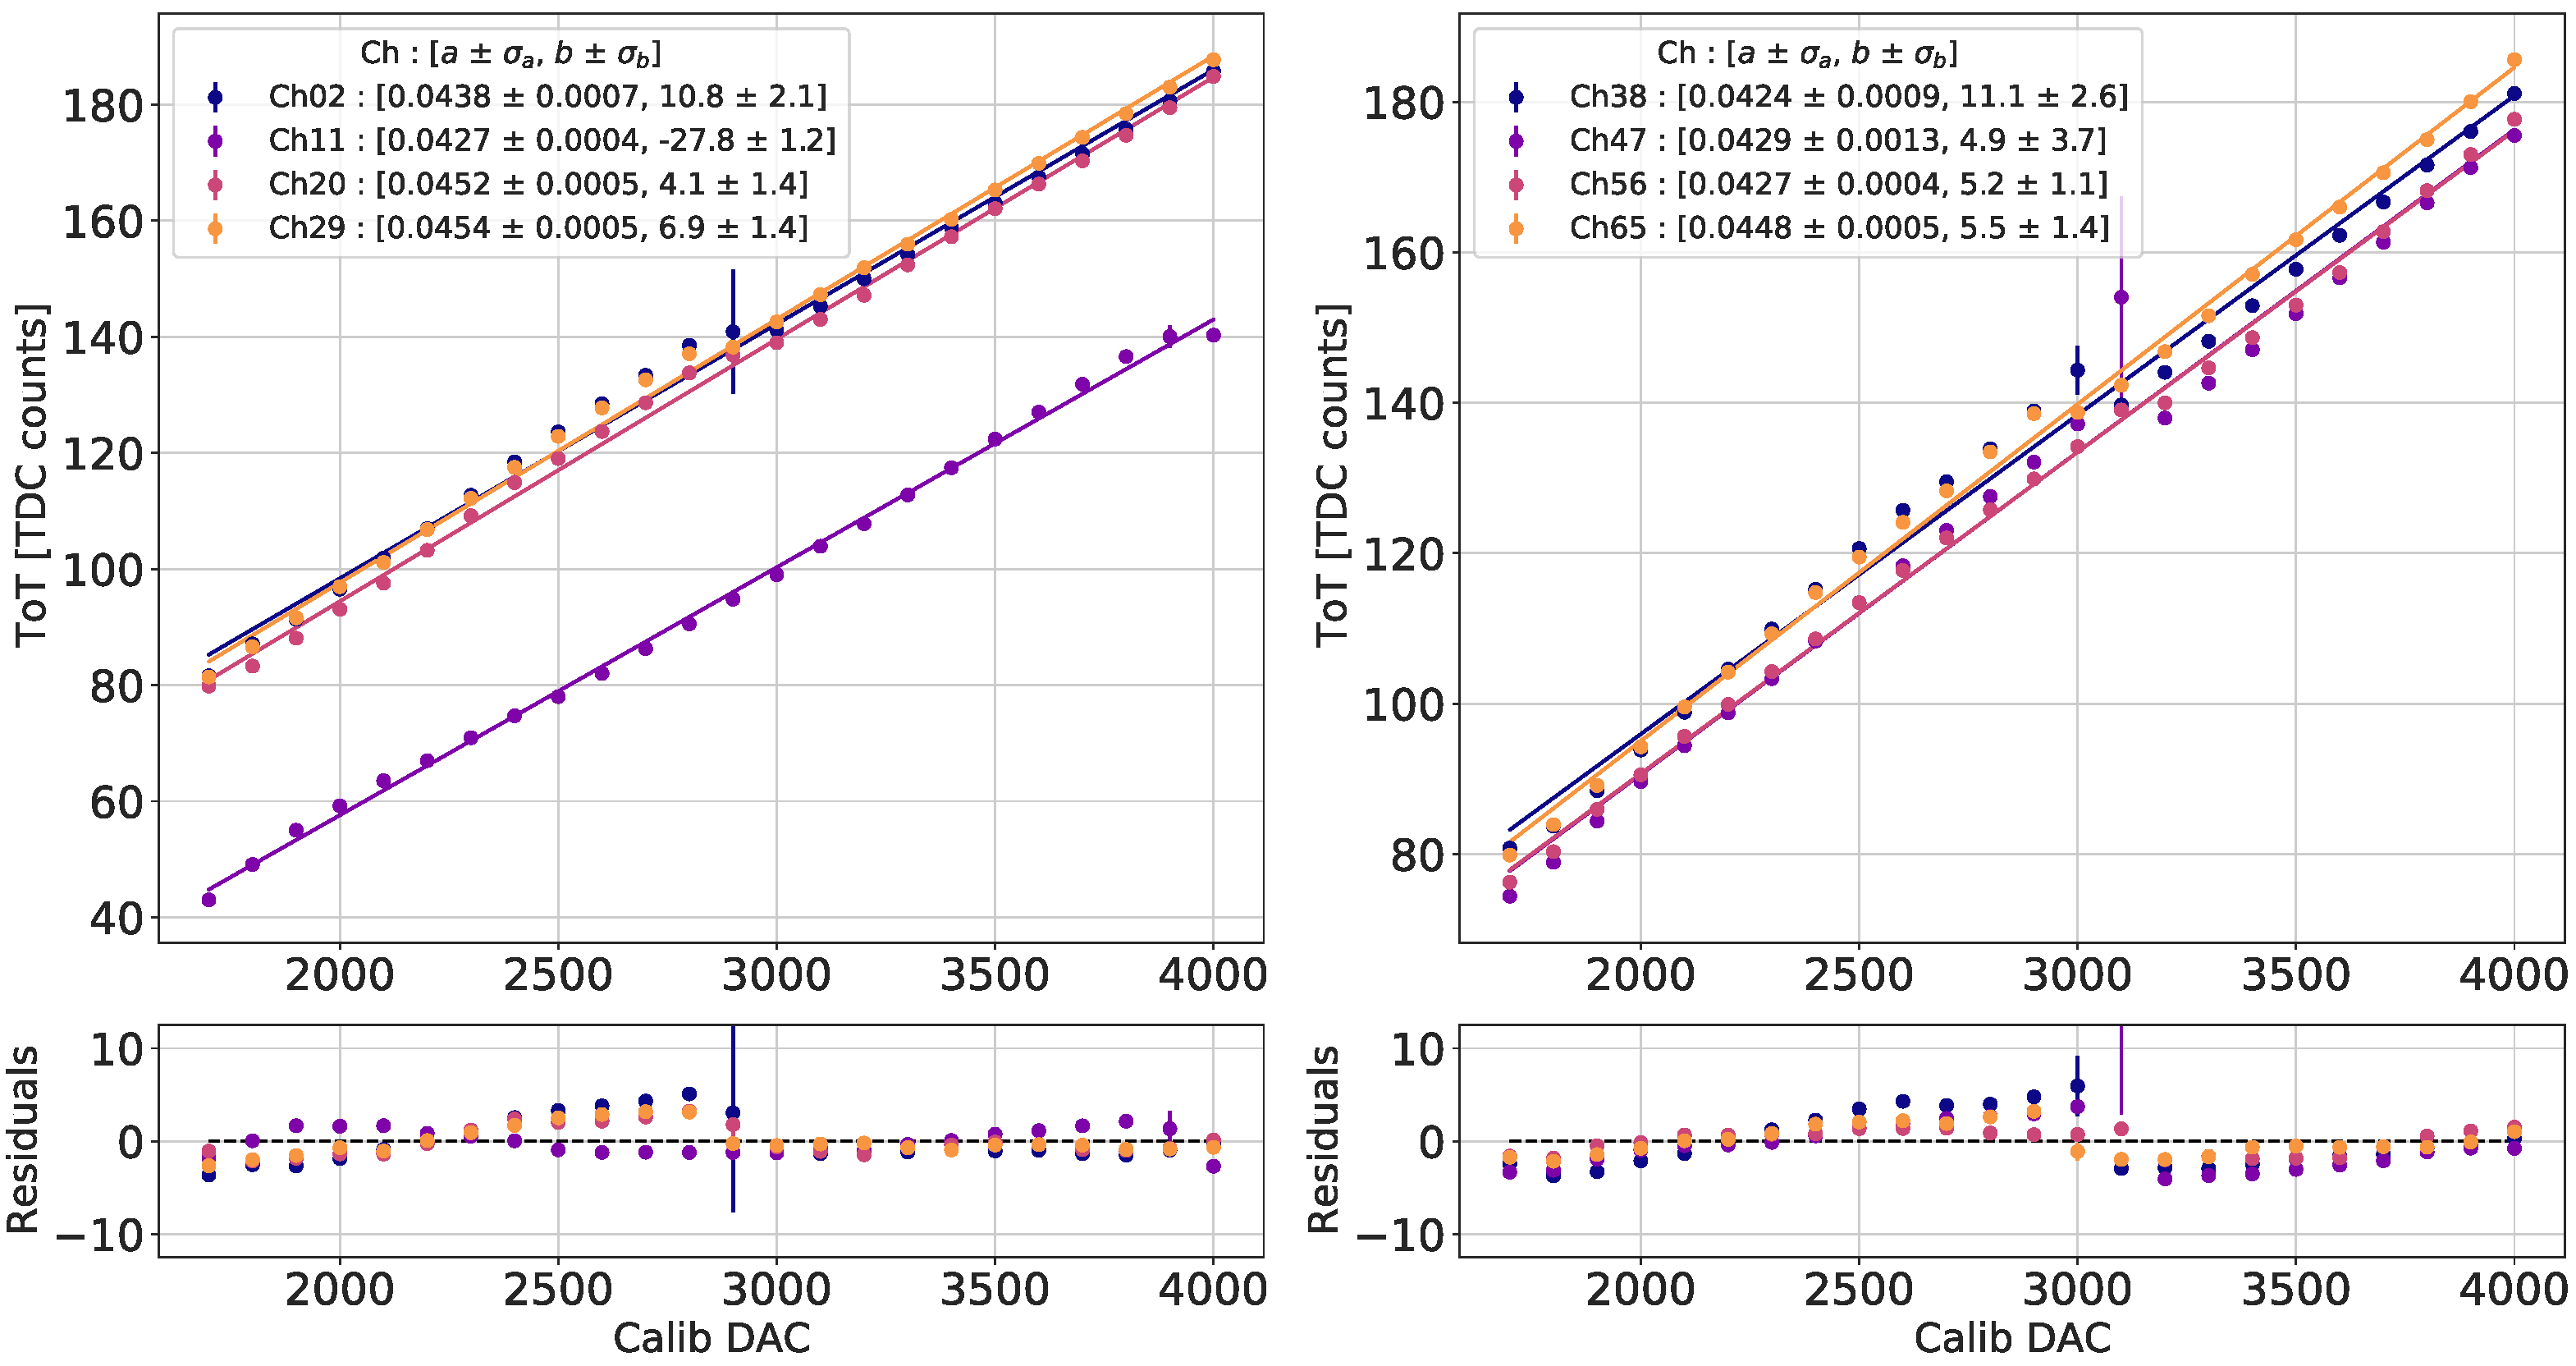
\includegraphics[width=0.75\linewidth]{Figures/HGCAL/TOT_Injection.pdf}
    \caption{The ToT response linearity to multiple injections corresponding to different \texttt{Calib\_DAC} values, defining the input charge. The  response is fitted with the linear function in Equation~\ref{eq:ADCLinearity} and the optimised parameters of the fit are reported in the legend.}
    \label{fig:TOT_Injection}
\end{figure}

\subsubsection{The ToA performance}
\label{subsubsec:The ToA performance}

The ToA measurements are crucial in discriminating pile-up events and improving particle identification in collision scenarios. Time measurements aim to achieve accurate timing alongside most of the charge information. The H2GCROCv3 ASIC allows configuring a single global phase and bunch crossing (BX) for data acquisition. Figure 5.36 presents TOA values for dif- ferent BX and phases and the corresponding ADC values for each time measurement. As observed, the time data depends on the sampling time. Ideally, the TOA measurement is more effective and linear when taken in the middle of the rising slope of the ADC signal. However, to measure charge efficiently, it is necessary to select the peak of the ADC signal. This selection significantly impacts time measurements for slower signals from large SiPM detectors. If the si- gnal starts within one BX and reaches its peak two BX later, the time walk of the measurement will exceed the limit, making it challenging to correlate with the correct charge measurement.

The 40 MHz HGCAL frequency requires configuring the ASIC to produce a TOA time walk below 25 ns. Detectors with lower capacitance exhibit shorter time walk times, while those with higher capacitance approach the 25 ns limit due to their slower signal generation. Figure 5.36 depicts the system’s time walk and associated jitter without any capacitor or detector connected at the input. The time walk generated is approximately 16 ns, producing a jitter below 100 ps for charge values of around 20 pC or higher. The fit of the time walk follows Equation 5.4.3, and the fit of the jitter follows Equation 58.
When the signal duration is extended, the optimal phase for charge measurement may result in poorer jitter performance. The capability to set different measurement phases for TDCs and ADCs will address BX information discrepancies in future ASIC versions. Finally, Figure 5.37 presents the TOA performance with the correct phase for time measurements, demonstrating the performance variations for different detector capacitances corresponding to SiPM sizes in HGCAL.
Furthermore, the increase in noise caused by larger detector capacitances impacts the minimum threshold value available for configuration and significantly affects the resolution of small charge injections. Figure 5.38 illustrates the TOA efficiency for a charge injection scan using different detector capacitances. The minimal charge that achieves TOA data with an efficiency of one varies for each SiPM size (see Figure 5.39). The three SiPM sizes allow for TOA data measurements from minimal charges of approximately 220 fC, 270 fC, and 380 fC, respectively. The system achieves a resolution of less than 100 ps, reaching a floor of 25 ps with all detectors. Nevertheless, increasing the detector capacitance affects the jitter for small charge injection and delays achieving 100 ps and 25 ps resolutions.

\begin{figure}
    \centering
    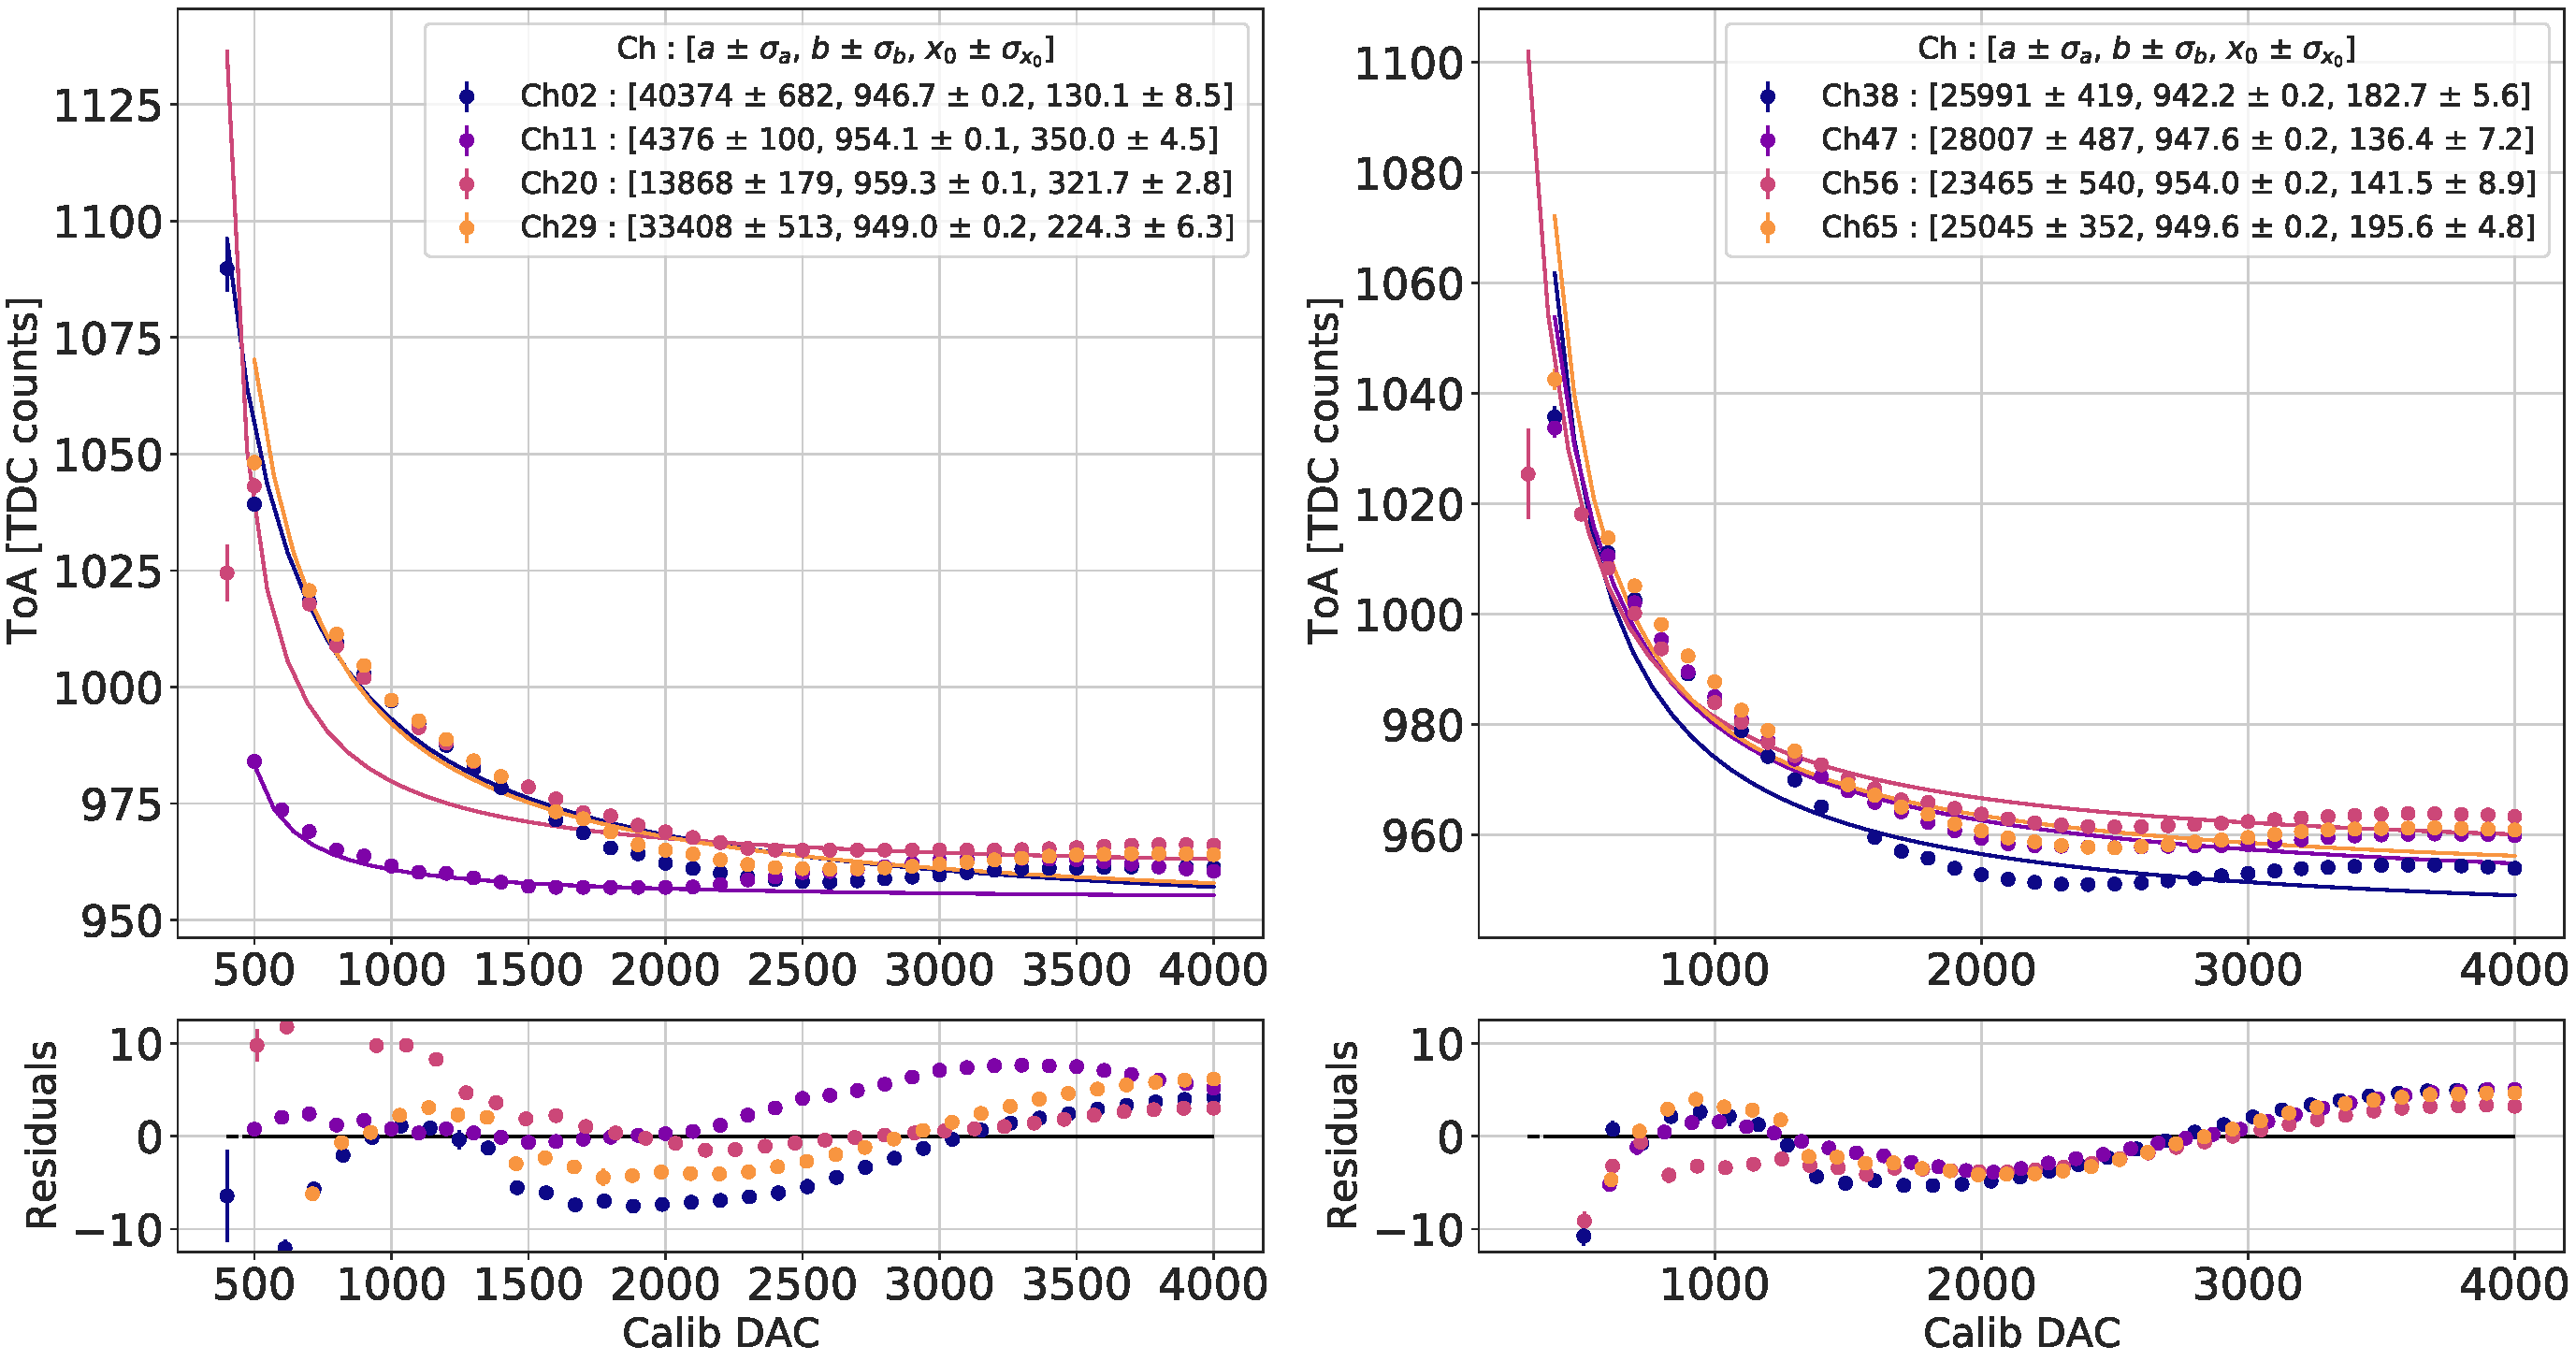
\includegraphics[width=0.75\linewidth]{Figures/HGCAL/TOA_Injection.pdf}
    \caption{}
    \label{fig:TOA_Injection}
\end{figure}

\begin{figure}
    \centering
    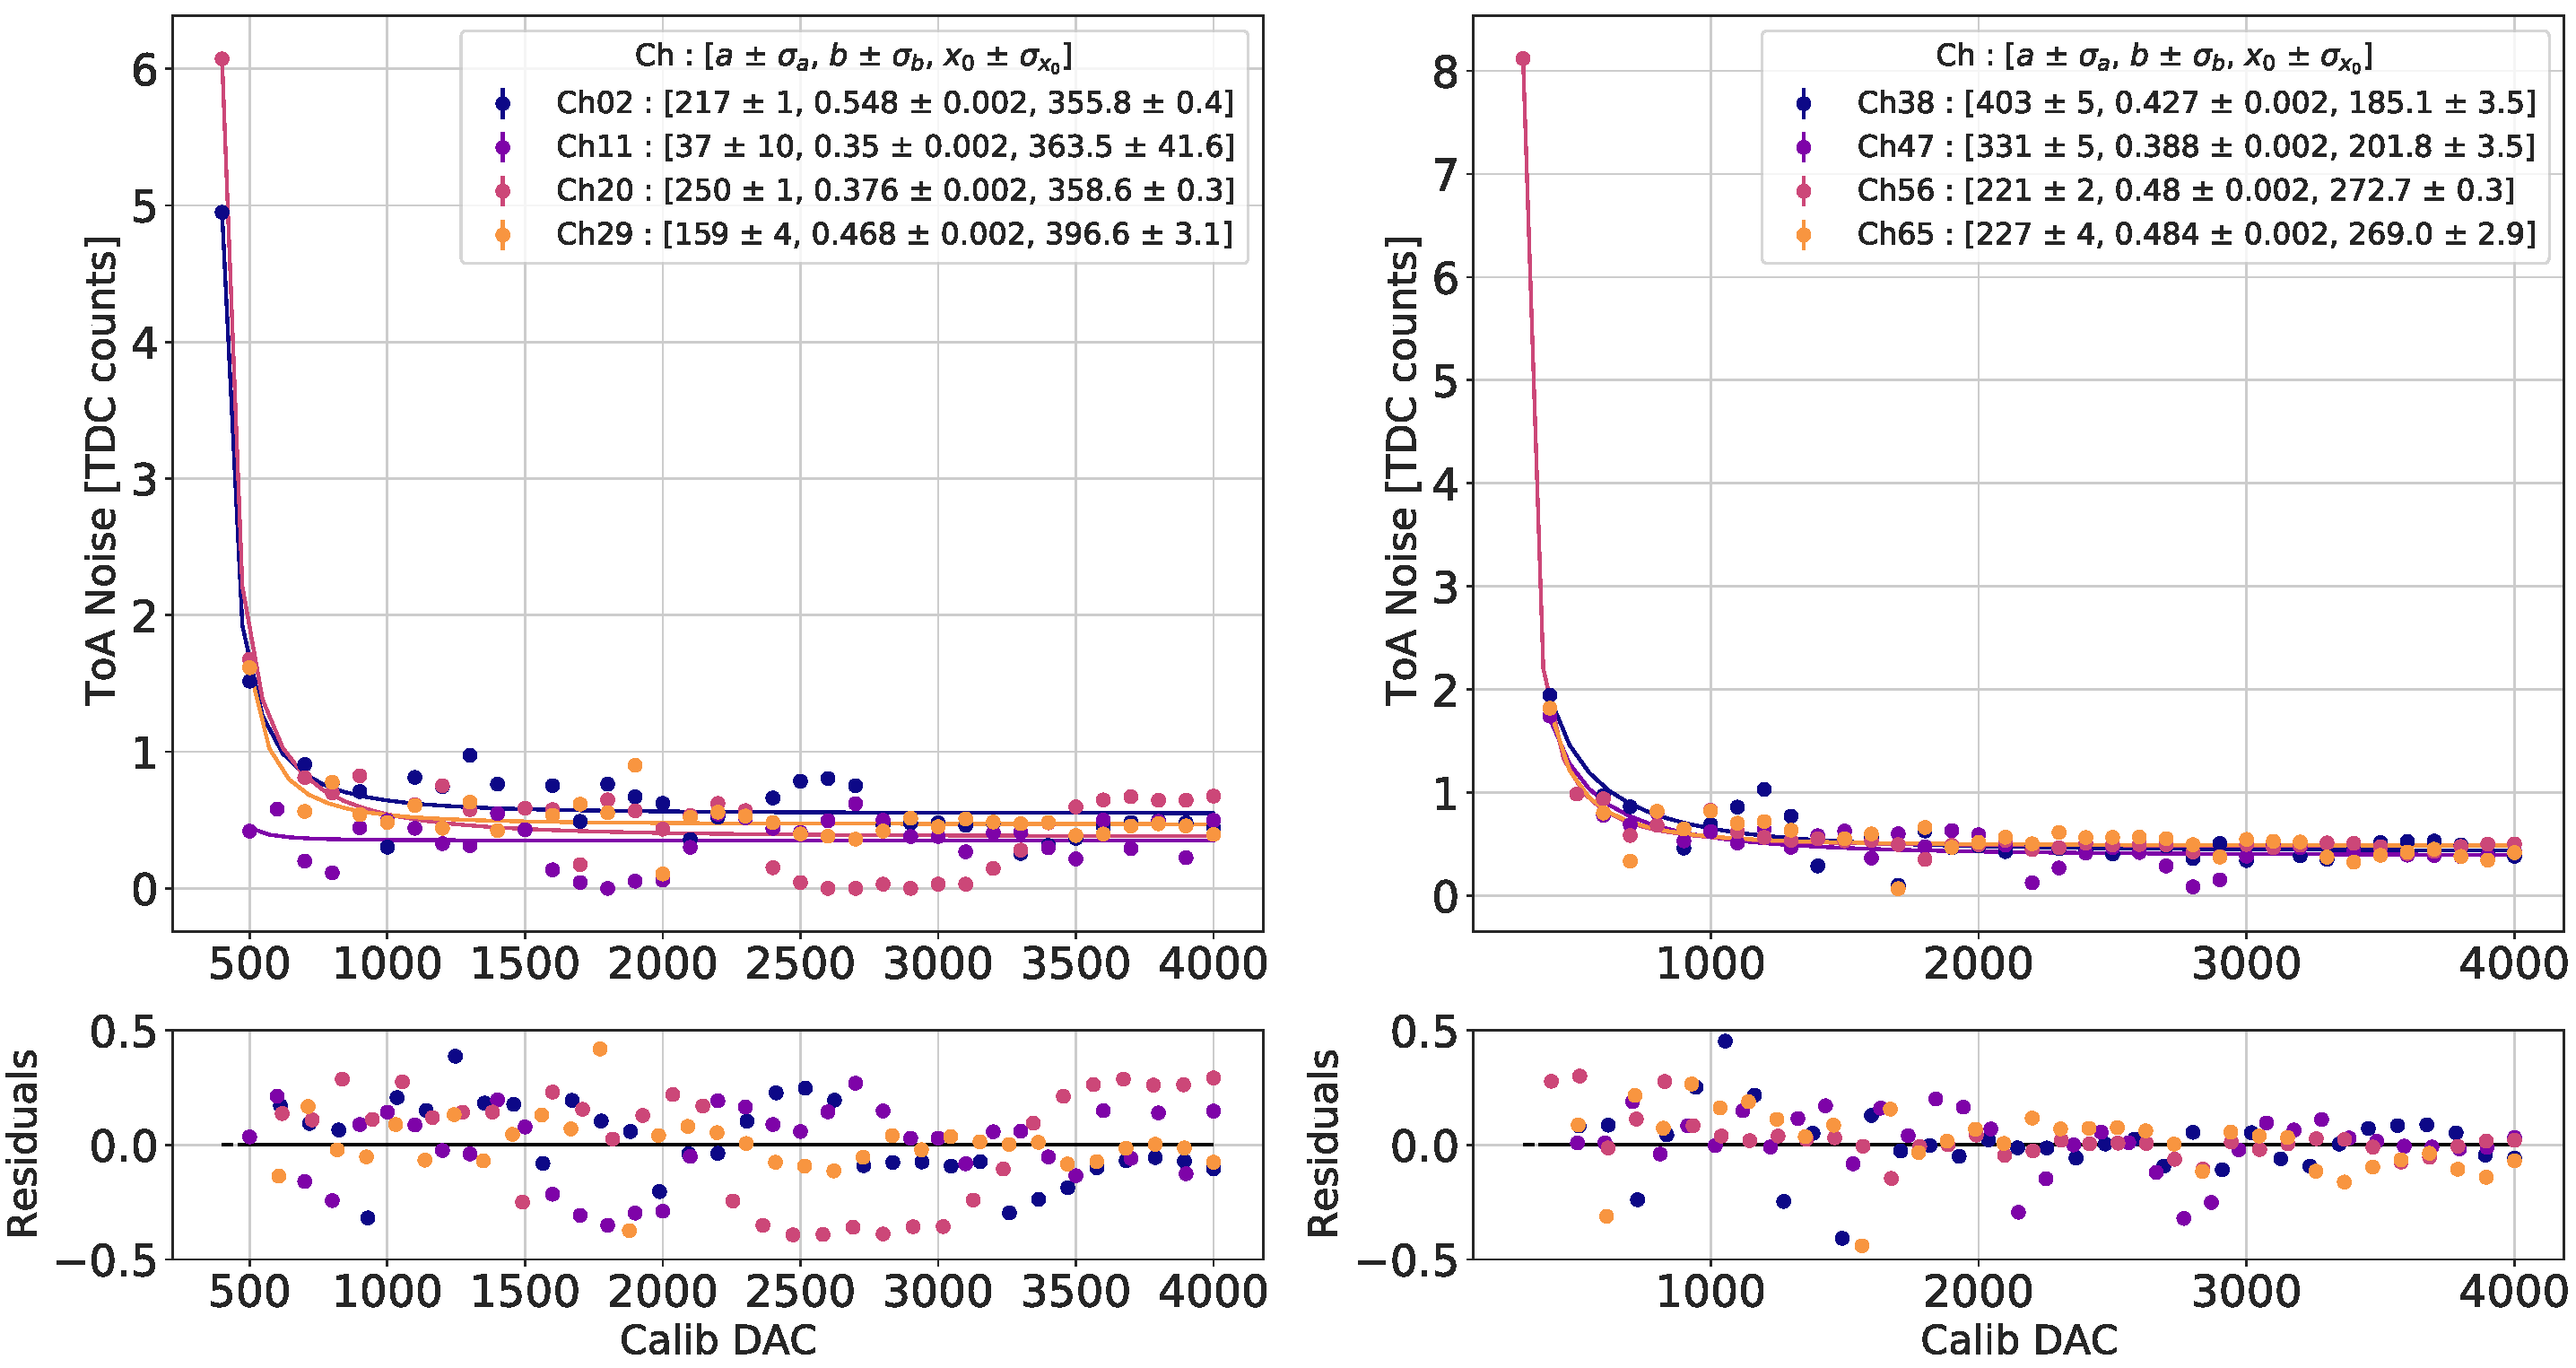
\includegraphics[width=0.75\linewidth]{Figures/HGCAL/ToANoise_Injection.pdf}
    \caption{}
    \label{fig:TOANoise_Injection}
\end{figure}

% The injection scan is the last test and provides the recorded ADC, ToA and ToT for different amplitudes of the injected signal. The ADC injection scan measures the ADC value of the signal peak. We can change the amplitude of the injected signal through the CalibDAC parameter inside the configuration. I put a graphic example on the left plot with three different signals and the three measured ADC. Of course what we expect is a linear dependence between the CalibDAC parameter and the recorded ADC.

% The ToA injection scan measures the time of arrival of the signal. The ToA is the instant of time at which the signal amplitude exceeds a threshold value. You can see from the exemple that a smaller signal amplitude provides a bigger ToA, while a higher signal amplitude leads to a smaller ToA. This is reflected in the right plot, where we can see the so-called “time walk”.


